%-------------------------------------------------------------------------------
% This file provides a skeleton ATLAS document.
%-------------------------------------------------------------------------------
% \pdfoutput=1
% The \pdfoutput command is needed by arXiv/JHEP/JINST to ensure use of pdflatex.
% It should be included in the first 5 lines of the file.
%-------------------------------------------------------------------------------
% Specify where ATLAS LaTeX style files can be found.
\newcommand*{\ATLASLATEXPATH}{latex/}
% Use this variant if the files are in a central location, e.g. $HOME/texmf.
% \newcommand*{\ATLASLATEXPATH}{}
%-------------------------------------------------------------------------------
\documentclass[UKenglish,texlive=2020]{\ATLASLATEXPATH atlasdoc}
\usepackage{multirow}
% The language of the document must be set: usually UKenglish or USenglish.
% british and american also work!
% Commonly used options:
%  texlive=YYYY          Specify TeX Live version (2013 is default).
%  atlasstyle=true|false Use ATLAS style for document (default).
%  coverpage             Create ATLAS draft cover page for collaboration circulation.
%                        See atlas-draft-cover.tex for a list of variables that should be defined.
%  cernpreprint          Create front page for a CERN preprint.
%                        See atlas-preprint-cover.tex for a list of variables that should be defined.
%  PAPER                 The document is an ATLAS paper (draft).
%  CONF                  The document is a CONF note (draft).
%  PUB                   The document is a PUB note (draft).
%  BOOK                  The document is of book form, like an LOI or TDR (draft)
%  txfonts=true|false    Use txfonts rather than the default newtx - needed for arXiv submission.
%  paper=a4|letter       Set paper size to A4 (default) or letter.

%-------------------------------------------------------------------------------
% Extra packages:
\usepackage{\ATLASLATEXPATH atlaspackage}
% Commonly used options:
%  biblatex=true|false   Use biblatex (default) or bibtex for the bibliography.
%  backend=biber         Use the biber backend rather than bibtex.
%  subfigure|subfig|subcaption  to use one of these packages for figures in figures.
%  minimal               Minimal set of packages.
%  default               Standard set of packages.
%  full                  Full set of packages.
%-------------------------------------------------------------------------------
% Style file with biblatex options for ATLAS documents.
\usepackage{\ATLASLATEXPATH atlasbiblatex}

% Package for creating list of authors and contributors to the analysis.
\usepackage{\ATLASLATEXPATH atlascontribute}

% Useful macros
\usepackage{\ATLASLATEXPATH atlasphysics}

\usepackage{\ATLASLATEXPATH atlascover}
% See doc/atlas_physics.pdf for a list of the defined symbols.
% Default options are:
%   true:  journal, misc, particle, unit, xref
%   false: BSM, heppparticle, hepprocess, hion, jetetmiss, math, process, other, texmf
% See the package for details on the options.

% Files with references for use with biblatex.
% Note that biber gives an error if it finds empty bib files.
\addbibresource{FCNCsupport.bib}
\addbibresource{bibtex/bib/PubNotes.bib}
\addbibresource{bibtex/bib/ATLAS.bib}
\addbibresource{bibtex/bib/CMS.bib}

% Paths for figures - do not forget the / at the end of the directory name.
\graphicspath{{logos/}{figures/}}

% Add you own definitions here (file FCNCsupport-defs.sty).
\usepackage{FCNCsupport-defs}
\usepackage{FCNCpaths}
\usepackage{lscape}
\usepackage{float}
%for sidewaystable added by Michel 2017-05-11
\usepackage{rotating}
\usepackage{longtable}
\usepackage[export]{adjustbox}
\usepackage{titlesec}
\usepackage{savesym}
\savesymbol{checkmark}
\usepackage{dingbat}
\usepackage{siunitx}
\usepackage{adjustbox}
\setcounter{secnumdepth}{4}

%-------------------------------------------------------------------------------
% Generic document information
%-------------------------------------------------------------------------------

% Title, abstract and document 
%-------------------------------------------------------------------------------
% This file contains the title, author and abstract.
% It also contains all relevant document numbers used by the different cover pages.
%-------------------------------------------------------------------------------

% Title
\AtlasTitle{\boldmath Search for flavor-changing neutral currents $tHq$ interactions with $H\to\taup\taum$ in proton-proton collisions at $\sqrt{s}=13$~TeV}

% Author - this does not work with revtex (add it after \begin{document})
\author{The ATLAS Collaboration}

% Authors and list of contributors to the analysis
% \AtlasAuthorContributor also adds the name to the author list
% Include package latex/atlascontribute to use this
% Use authblk package if there are multiple authors, which is included by latex/atlascontribute
% \usepackage{authblk}
% Use the following 3 lines to have all institutes on one line
% \makeatletter
% \renewcommand\AB@affilsepx{, \protect\Affilfont}
% \makeatother
% \renewcommand\Authands{, } % avoid ``. and'' for last author
% \renewcommand\Affilfont{\itshape\small} % affiliation formatting
% \AtlasAuthorContributor{First AtlasAuthorContributor}{a}{Author's contribution.}
% \AtlasAuthorContributor{Second AtlasAuthorContributor}{b}{Author's contribution.}
% \AtlasAuthorContributor{Third AtlasAuthorContributor}{a}{Author's contribution.}
% \AtlasContributor{Fourth AtlasContributor}{Contribution to the analysis.}
% \author[a]{First Author}
% \author[a]{Second Author}
% \author[b]{Third Author}
% \affil[a]{One Institution}
% \affil[b]{Another Institution}

% If a special author list should be indicated via a link use the following code:
% Include the two lines below if you do not use atlasstyle:
% \usepackage[marginal,hang]{footmisc}
% \setlength{\footnotemargin}{0.5em}
% Use the following lines in all cases:
% \usepackage{authblk}
% \author{The ATLAS Collaboration%
% \thanks{The full author list can be found at:\newline
%   \url{https://atlas.web.cern.ch/Atlas/PUBNOTES/ATL-PHYS-PUB-2016-007/authorlist.pdf}}
% }

% Draft version:
% Should be 1.0 for the first circulation, and 2.0 for the second circulation.
% If given, adds draft version on front page, a 'DRAFT' box on top of each other page, 
% and line numbers.
% Comment or remove in final version.
\AtlasVersion{16}

% ATLAS reference code, to help ATLAS members to locate the paper
%\AtlasRefCode{GROUP-2017-XX}

% ATLAS note number. Can be an COM, INT, PUB or CONF note
% \AtlasNote{ATLAS-CONF-2016-XXX}
% \AtlasNote{ATL-PHYS-PUB-2016-XXX}
% \AtlasNote{ATL-COM-PHYS-2016-XXX}

% CERN preprint number
% \PreprintIdNumber{CERN-PH-2016-XX}

% ATLAS date - arXiv submission; usually filled in by the Physics Office
% \AtlasDate{\today}

% ATLAS heading - heading at top of title page. Set for TDR etc.
% \AtlasHeading{ATLAS ABC TDR}

% arXiv identifier
% \arXivId{14XX.YYYY}

% HepData record
% \HepDataRecord{ZZZZZZZZ}

% Submission journal and final reference
% \AtlasJournal{Phys.\ Lett.\ B.}
% \AtlasJournalRef{\PLB 789 (2014) 123}
% \AtlasDOI{}

% Abstract - % directly after { is important for correct indentation
\AtlasAbstract{%
A search is presented for flavor-changing neutral currents $tHq$ interactions with $H\to\taup\taum$ using a data set collected with the ATLAS detector at the LHC, corresponding to an integrated luminosity of $140$~fb$^{-1}$ of proton-proton collisions at a center-of-mass energy of 13~TeV. The search is performed in the decay chain $t\bar{t} \to Wb+Hq$ or $qg \to tH \to Wb+H$ ($q=c/u$), where the $W$ boson decays inclusively and H decays to $\taup\taum$. Upper limits at 95~\% confidence level for the coupling coefficient are measured to be $XXX$ and $XXX$, while the expected limits are $XXX^{+XXX}_{-XXX}\%$ and $XXX^{+XXX}_{-XXX}\%$, respectively.

}
%-------------------------------------------------------------------------------
% The following information is needed for the cover page. The commands are only defined
% if you use the coverpage option in atlasdoc or use the atlascover package
%-------------------------------------------------------------------------------

% List of supporting notes  (leave as null \AtlasCoverSupportingNote{} if you want to skip this option)
 \AtlasCoverSupportingNote{Support note}{https://cds.cern.ch/record/2687866/}
% \AtlasCoverSupportingNote{Short title note 2}{https://cds.cern.ch/record/YYYYYYY}
%
% OR (the 2nd option is deprecated, especially for CONF and PUB notes)
%
% Supporting material TWiki page  (leave as null \AtlasCoverTwikiURL{} if you want to skip this option)
% \AtlasCoverTwikiURL{https://twiki.cern.ch/twiki/bin/view/Atlas/WebHome}

% Comment deadline
% \AtlasCoverCommentsDeadline{DD Month 2016}

% Analysis team members - contact editors should no longer be specified
% as there is a generic email list name for the editors
% \AtlasCoverAnalysisTeam{Peter Analyser, Susan Editor1, Jenny Editor2, Alphonse Physicien}

% Editorial Board Members - indicate the Chair by a (chair) after his/her name
% Give either all members at once (then they appear on one line), or separately
% \AtlasCoverEdBoardMember{EdBoard~Chair~(chair), EB~Member~1, EB~Member~2, EB~Member~3}
% \AtlasCoverEdBoardMember{EdBoard~Chair~(chair)}
% \AtlasCoverEdBoardMember{EB~Member~1}
% \AtlasCoverEdBoardMember{EB~Member~2}
% \AtlasCoverEdBoardMember{EB~Member~3}

% A PUB note has readers and not an EdBoard -- give their names here (one line or several entries)
% \AtlasCoverReaderMember{Reader~1, Reader~2}
% \AtlasCoverReaderMember{Reader~1}
% \AtlasCoverEdBoardMember{Reader~2}

% Editors egroup
% \AtlasCoverEgroupEditors{atlas-GROUP-2016-XX-editors@cern.ch}

% EdBoard egroup
% \AtlasCoverEgroupEdBoard{atlas-GROUP-2016-XX-editorial-board@cern.ch}


% Author and title for the PDF file
\hypersetup{pdftitle={ATLAS document},pdfauthor={The ATLAS Collaboration}}
%-------------------------------------------------------------------------------
% Content
%-------------------------------------------------------------------------------
\begin{document}

\maketitle

\tableofcontents

\newpage

% List of contributors - print here or after the Bibliography.
%\begin{itemize}
%\item Boyang Li: main analyser, analysis code maintainer; signal generation; derivation, ntuple production; fake tau estimation; BDT analysis; systematics; fit; support note.
%\item Weiming Yao: Analysis contact, main analyser, \texttt{ttHML} ntuple skimming and support; fake tau estimation; BDT analysis; cross check; support note.
%\item MingMing Xia: Analysis contact, main analyser, \texttt{xTauFramework} n-tuple production; production validation; fake tau estimation in hadronic channels; systematic and final fits.
%\item Xin Chen: Supervisor of Boyang Li and MingMing Xia
%\end{itemize}
\PrintAtlasContribute{0.30}
\clearpage
\newpage

\linenumbers
\section{To do list}

Add signal samples used by FCNC $H\to multilepton$ group (Their AOD files are deleted, still not available).

<<<<<<< HEAD
Add signal samples used by FCNC $H\to \gamma\gamma/bb$ group.
%%PLIV has been implemented since tthW V2.
%PLIV implementation.
=======
\sout{PLIV implementation.}(Turns out it's already applied.)

The n-tuples are ready, started working on:
>>>>>>> 737ca77df1863287c5810eb46ad1229333e37168

Implementation of theory systematics and instrumental systematics. Including:

\begin{itemize}
	\item JES, JER
	\item flavor tagging
	\item JVT
	\item MET\_SoftTrk
	\item PRW
	\item Tau reconstruction, selection, identification, electron veto, TES
	\item Renormalisation and factorisation scale
	\item PDF
	\item $\ttbar$ and V+jets cross section
	\item ISR and FSR
\end{itemize}

Leptonic channels specific:
\begin{itemize}
	\item Lepton trigger SF
	\item Electron reconstruction, identification, isolation
	\item Muon identification, isolation
	\item EG\_RESOLUTION, EG\_SCALE
\end{itemize}

Hadronic channels specific:
\begin{itemize}
	\item Tau trigger SF
\end{itemize}

\section{Change log}

\subsection{From V1 to V2}

Leptonic channels:  80fb-1 $\to$ 140fb-1

BDT tau ID $\to$ RNN tau ID

Updates to PFlow jets with DL1r b-tagging.

Optimised event seletion.

Changed fake estimation method.

Added signal regions $l\tau$ 1j and $l\tau$ 2j.

\subsection{From V2 to V3}

Added to do list and change log.

Added Analysis outline section and moved signal region definition here.

Added yield tables for CRs.

Added plots for the variables defined.

Added closure test for ABCD method.

BDT optimisation.

<<<<<<< HEAD
\subsection{From V3 to V3.1}

Made the note more readable by introducing new names for SR and CR.

...
=======
\subsection{From V3 to V4}

Updated n-tuples with full systematics (ttWML n-tuple V6).

Improved figures, clarified a few statements.
>>>>>>> 737ca77df1863287c5810eb46ad1229333e37168

\section{Introduction}
Since the discovery of the Higgs boson in 2012, great efforts are made to study its properties. As the mass of the Higgs boson is about 125 GeV \cite{HiggsMass}, it is kinematically allowed that a top quark decays to a Higgs boson and an up-type quark via the flavour-changing neutral current (FCNC). In the Standard Model (SM), the FCNC interaction is forbidden at tree level and suppressed at higher orders due to the Glashow-Iliopoulos-Maiani (GIM) mechanism \cite{GIM}. The $t\to u/c+H$ branching fraction in the SM is calculated to be around $10^{-15}$ \cite{brtch3}. It would be enhanced in many models beyond the SM (BSM). Examples are the quark-singlet model \cite{quarkSinglet1,quarkSinglet2}, the two-Higgs doublet model with or without the flavour violation \cite{2hdm1,2hdm2}, the minimal supersymmetric standard model (MSSM) \cite{2hdm3}, supersymmetry with R-parity violation \cite{Rparity},
the Topcolour-assisted Technicolour model \cite{Techni} or models with warped extra dimensions \cite{extraD}, the little Higgs model with T-parity conservation \cite{littleH} and the composite Higgs models \cite{compositeH}.
Especially, the ansatz of Cheng and Sher \cite{Sher} allows a branching fraction of about $10^{-3}$ \cite{FCNC_rate}. Therefore, an observation of this decay would be a clear evidence for new physics.

On the other hand, if the $tHq$ interaction exists, the single-top, Higgs associated production through this interaction should also be enhanced. The $tH$ associated production in the SM prediction is expected to be small at LHC\cite{tHjb_production}. So the study on this process will also contribute to the FCNC interaction searches.

Upper $95\%$ CL limits on BR($t\to Hq$) have been obtained by ATLAS based on the data from 2015 and 2016, in the $H\to\gamma\gamma$ \cite{fcncgmgm}, $H\to WW/\tll$ multilepton \cite{fcncml} and  $\Htautau$, $H\to b\bar{b}$ \cite{fcnctautau} channels. The combined expected (observed) limits are $0.083\%$ ($0.11\%$) and $0.083\%$ ($0.12\%$) for $t\to Hc$ and $t\to Hu$, respectively.

The $t\to Hq$ decay and $gq\to tH$ production are also searched by CMS based on the data from 2015 and 2016\cite{CMS-TOP-17-003}. 

The FCNC coupling is parametrised using dim-6 operators \cite{fcnc_production_theory}. The effective Lagrangian regarding $tqH$ interaction before spontaneously symmetry breaking is:
%
\begin{equation}
\mathcal{L}_{EFT} = \frac{C^{i3}_{u\phi}}{\Lambda^{2}}(\phi^{\dagger}\phi)(\bar{q_{i}}t)\tilde{\phi} + \frac{C^{3i}_{u\phi}}{\Lambda^{2}}(\phi^{\dagger}\phi)(\bar{Q}u_{i})\tilde{\phi} + H.c
\label{eq:eq01}
\end{equation}
%

Where the the operator notation is consistent with \cite{fcnc_production_theory}. $C^{i3}$ is the Wilson coefficient of the 6-dim operator with $i=1,2$ denoting the flavor of upper type quark. $\Lambda$ is the scale of the new physics where the UV cut off happens which is set as 1~TeV as benchmark. $\phi$ is the SM higgs doublet. $\tilde{\phi}=\epsilon\phi^\ast$ where $\epsilon$ is the antisymmetric matrix with $\epsilon_{12}=-\epsilon_{21}=1$.

The Wilson coefficient $C_{u\phi}$'s can be extracted as
\begin{equation}
\begin{array}{l}
(C^{i3}_{u\phi})^2 + (C^{3i}_{u\phi})^2 = 1946.6~\text{BR}(t\to qH)\\
(C^{13}_{u\phi})^2 + (C^{31}_{u\phi})^2 = \sigma(ug\to tH)/365.2~\text{fb}\\
(C^{23}_{u\phi})^2 + (C^{32}_{u\phi})^2 = \sigma(cg\to tH)/52.9~\text{fb}
\end{array}
\label{eq:eq02}
\end{equation}

To give a better impression on the numbers, we use $\text{BR}(t\to qH)=1(0.2)\%$ as benchmark, which is corresponding to ($C^{13}_{u\phi})^2 + (C^{31}_{u\phi})^2=19.47(3.89)$, $\sigma(ug\to tH)=7109.0(1421.8)$ pb, $\sigma(cg\to tH)=1029.8(206.0)$ pb.

In this article, a search for the decay $t\to qH$ in the $t\bar{t}$ production (TT) and single-top, Higgs associated production (ST) with $H\to\tau\tau$  as shown in Fig \ref{fig:diagrams} using 140~fb$^{-1}$ of proton-proton collision data at 13~TeV, taken with the ATLAS detector at the Large Hadron Collider (LHC), is presented. The final state is characterized by one top and one Higgs. In TT, there is an additional u/c quark forming a top resonance with Higgs.

\begin{figure}[htb]
\centering
\includegraphics[width=0.4\textwidth]{../FCNCFigures/r21/diagrams/TT.pdf}
\includegraphics[width=0.4\textwidth]{../FCNCFigures/r21/diagrams/ST.pdf}\\
\caption{ Diagrams of FCNC TT(left) and ST(right) process. }
\label{fig:diagrams}
\end{figure}


\section{Detector, data set and Monte Carlo simulation}

\subsection{ATLAS detector}
\label{sec:detector}

The ATLAS detector \cite{PERF-2007-01} at the LHC covers nearly the entire solid angle around the collision point. It consists of an inner tracking detector surrounded by a thin superconducting solenoid, electromagnetic and hadronic calorimeters, and a muon spectrometer incorporating three large superconducting toroid magnets.

The inner-detector system (ID) is immersed in a \SI{2}{T} axial magnetic field and provides charged particle tracking in the range $| \eta | < 2.5$. A high-granularity silicon pixel detector covers the vertex region and typically provides three measurements per track. It is followed by a silicon microstrip tracker, which usually provides four two-dimensional measurement points per track. These silicon detectors are complemented by a transition radiation tracker, which enables radially extended track reconstruction up to $| \eta | < 2.0$. The transition radiation tracker also provides electron identification information based on the fraction of hits above a higher energy-deposit threshold corresponding to transition radiation. Compared to Run-1, an Insertable B-Layer \cite{IBL} (IBL) is inserted as the innermost pixel layer during LS1 for Run-2, which significantly improves the tracking performance.

The calorimeter system covers the pseudorapidity range $| \eta | < 4.9$. Within the region $| \eta | < 3.2$, electromagnetic calorimetry is provided by barrel and endcap high-granularity liquid-argon (LAr) electromagnetic calorimeters, with an additional thin LAr presampler covering $| \eta | < 1.8$, to correct for energy loss in material upstream of the calorimeters. Hadronic calorimetry is provided by a scintillator-tile calorimeter, segmented into three barrel structures within $| \eta | < 1.7$, and two LAr hadronic endcap calorimeters.

A muon spectrometer (MS) comprises separate trigger and high-precision tracking chambers measuring the deflection of muons in a magnetic field generated by superconducting air-core toroids. The precision chamber system covers the region $| \eta |< 2.7$ with three layers of monitored drift tubes, complemented by cathode strip chambers in the forward region, where the background is highest. The muon trigger system covers the range $| \eta | < 2.4$ with resistive-plate chambers in the barrel, and thin-gap chambers in the endcap regions.

\subsection{Data set}
\label{sec:dataset}

This analysis is based on the full proton-proton data at a center-of-mass energy $\sqrt{s}=13$~TeV with a bunch spacing of 25~ns collected by ATLAS in Run-2. The following good run list (GRL) was used for the 2015 dataset:


{\tt\scriptsize data15\_13TeV.periodAllYear\_DetStatus-v89-pro21-02\_Unknown\_PHYS\_StandardGRL\_All\_Good\_25ns.xml}

which corresponds to an integrated luminosity of 3.22 fb$^{-1}$.

The GRL used for the 2016 dataset:

{\tt\scriptsize data16\_13TeV.periodAllYear\_DetStatus-v89-pro21-01\_DQDefects-00-02-04\_PHYS\_StandardGRL\_All\_Good\_25ns.xml}

corresponds to an integrated luminosity of 32.88 fb$^{-1}$.

These GRLs exclude data where the IBL was not fully operational. The uncertainty in the combined 2015+2016 integrated luminosity, 36.1~fb$^{-1}$, is $2.1\%$. It is derived, following a methodology similar to that detailed in Ref.~\cite{DAPR-2013-01}, from a calibration of the luminosity scale using x-y beam-separation scans performed in August 2015 and May 2016.

The GRL used for the 2017 dataset:

{\tt\scriptsize data17\_13TeV.periodAllYear\_DetStatus-v99-pro22-01\_Unknown\_PHYS\_StandardGRL\_All\_Good\_25ns\_Triggerno17e33prim.xml}

corresponds to an integrated luminosity of 44.307 fb$^{-1}$.

The GRL used for the 2018 dataset:

{\tt\scriptsize  data18\_13TeV.periodAllYear\_DetStatus-v102-pro22-04\_Unknown\_PHYS\_StandardGRL\_All\_Good\_25ns\_Triggerno17e33prim.xml}

corresponds to an integrated luminosity of 59.937 fb$^{-1}$. The final luminosity used for the analysis is 140.45 fb$^{-1}$.
%The integrated luminosity is 36.1~fb$^{-1}$ with a relative uncertainty of 3.2\% after the application of data-quality requirements.
%The average number of interactions per bunch crossing, over short time periods of about 1 minute, denoted by $\langle\mu\rangle$, is 13 in 2015 and 25 in 2016. The pile-up background is formed by the inelastic collisions, producing mainly low transverse momentum particles, in addition to the hard interaction.

\subsection{Signal and background simulation}
\label{sec:generator}

The overview of the major samples generated is summarized in table \ref{mob}.

The TopFCNC UFO model \cite{FCNC_UFO1,FCNC_UFO2} with 5-flavour scheme is used for signal simulation.

The FCNC ST signal is simulated using MadGraph5\_aMC@NLO v2.6.2 \cite{MG5} interfaced with Pythia 8 \cite{Pythia8} with the A14 tune \cite{A14} for the generation of parton showers, hadronisation and multiple interactions and the NNPDF30NLO \cite{NNPDF30NLO} parton distribution functions (PDF) is used to generate $qg$ events at next-to-leading order (NLO) in QCD. Depending on either up quark or charm quark involved in the FCNC decay and either the $W$ bosons decaying hadronically or leptonically, 4 samples are generated for each term of effective Lagrangian, so eight samples in total.

The FCNC TT signal is simulated using Powheg-Box \cite{Powheg} V2 interfaced with Pythia8 \cite{Pythia8} with the A14 tune \cite{A14} for the generation of parton showers, hadronisation and multiple interactions and the NNPDF30NLO \cite{NNPDF30NLO} parton distribution functions (PDF) is used to generate $t\bar{t}$ events at next-to-leading order (NLO) in QCD. Depending on either the top or the anti-top quark decaying to $bW$, either up quark or charm quark involved in the FCNC decay and either the $W$ bosons decaying hadronically or leptonically, eight samples are produced with the Higgs going to a $\tau$-lepton pair.

The dominant background is the $t\bar{t}$ production. The $t\bar{t}$ process and the single top process are generated with Powheg-Box \cite{Powheg} V2, and Pythia8 is used for the parton shower. NNPDF30NLO \cite{NNPDF30NLO} and A14 tune \cite{A14} are used for $t\bar{t}$(single top). The $t\bar{t}$ sample is also generated with different generators and parton showers models, as well as different amount of radiations, for systematics as detailed in Sec. \ref{sec:systematics}.

The $t\bar{t}X$, where X=$W$, $ee$, $\mu\mu$, $\tau\tau$ or $Z(qq,\nu\nu)$ ($\tau\tau$ has the Higgs resonance excluded), are generated with MadGraph5\_aMC@NLO and inferfaced with Pythia8 for the parton shower. The NNPDF30NLO \cite{NNPDF30NLO} is used for the matrix element PDF. The $t\bar{t}$, single top and $t\bar{t}X$ are combined into a single process named top background in the analysis.

The $W$+jets, $Z$+jets and diboson backgrounds are simulated using Sherpa 2.2.1 \cite{Sherpa} with NNPDF30NNLO PDF \cite{NNPDF30NLO}.

The $\tau$ decay in the single top samples is handled by Tauola \cite{Tauola}. All samples showered by Pythia8 (Sherpa) have the $\tau$ decays also handled by Pythia8 (Sherpa). All the decay modes of the $\tau$ lepton are allowed in the event generators (but may be subject to generator filters). The summary of used generators for matrix element and parton shower is given in Tab. \ref{mob}.

The SM higgs background includes $ggH$, $VH$, $VBF$ and $t\bar{t}H$, generated from Powheg-Box \cite{Powheg} V2 interfaced with Pythia8. The overall contribution is pretty small. Various PDF and tune options are use for those samples depending on the decay modes.

The $tH$ associated production is negligible but we still considered it. The sample is generated using MadGraph5 and interfaced with pythia8 for parton shower. CT10 PDF and A14 tune are used. It is treated as part of SM higgs background explained in above.

All Monte-Carlo (MC) samples were passed through the full GEANT4 \cite{GEANT4} simulation of the ATLAS detector, except for two extra \ttbar samples with Pythia8 and Herwig7 \cite{Herwig} parton showering which are simulated with ATLFAST-II \cite{AFII} for systematics (Sec. \ref{sec:systematics}). In the analysis, the simulated events were reweighted based on their pile-up to match the pile-up profile observed in data.

The full list of MC samples and their corresponding cross sections are given in App. \ref{app:mc_sample_list}. The single boson and diboson cross sections are calculated to NNLO \cite{bosonXsec}. The $t\bar{t}$ cross section is calculated at NNLO in QCD including resummation of NNLL soft gluon terms for a top-quark mass of 172.5 GeV \cite{ttXsec}. The $t\bar{t}H$ and $t\bar{t}V$ are normalized to NLO cross sections according to \cite{HiggsBR} and \cite{ttVXsec}. The $t$-channel and $s$-channel single top cross sections are calculated at NLO with Hathor v2.1 \cite{Hather1,Hather2}, while the $Wt$ channel is calculated at NLO+NNLL \cite{WtXsec}.

\begin{table}
\footnotesize
\centering
\caption{Overview of the MC generators used for the main signal and background samples}
\begin{tabular}[h]{l|c|c|c|c|c|c}
\hline \hline
\multirow{2}{*}{Process} & \multicolumn{2}{c|}{Generator} & \multicolumn{2}{c|}{PDF set} & \multirow{2}{*}{Tune} & \multirow{2}{*}{Order} \\ \cline{2-5}
        &  ME   &  PS    &  ME  & PS &   &  \\\hline
TT Signal & Powheg & Pythia8 & NNPDF30NLO & NNPDF23LO & A14 & NLO \\ \hline
ST Signal & MadGraph5\_aMC@NLO & Pythia8 & NNPDF30NLO & NNPDF23LO & A14 & NLO \\ \hline
$W/Z$+jets & \multicolumn{2}{c|}{Sherpa 2.2.1} & \multicolumn{2}{c|}{NNPDF30NNLO} & Sherpa & NLO/LO \\ \hline
\ttbar & Powheg & Pythia8 & NNPDF30NLO & NNPDF23LO & A14 & NLO \\ \hline
Single top & Powheg & Pythia6 & CT10(NLO) & CTEQ6L1\cite{CTEQ} & Perugia2012 & NLO \\ \hline
$t\bar{t}X$ & MadGraph5\_aMC@NLO & Pythia8 & NNPDF30NLO & NNPDF23LO & A14 & NLO \\ \hline
Diboson & \multicolumn{2}{c|}{Sherpa 2.2.1} & \multicolumn{2}{c|}{NNPDF30NNLO} & Sherpa & NLO/LO \\ \hline\hline
\end{tabular}
\label{mob}
\end{table}


\section{Object reconstruction}
\label{sec:obj_reco}

In this section, various objects used in this analysis are defined, namely jets, electrons, muons, hadronically decaying taus and missing transverse energy. 

\subsection{Jets}
Jets are reconstructed using the anti-$k_t$ algorithm \cite{antikt} with a distance parameter $R=0.4$ applied to the particle flow candidates. Only jets with $\pt>25$~GeV and $|\eta|<4.5$ are considered by the analysis. To suppress jets produced in additional pile-up interactions, jets with $\pt<60$~GeV and $|\eta|<2.4$ are required to have a Jet Vertex Tagger (JVT \cite{JVT}) parameter larger than 0.2 (Medium working point). The JVT is the output of the jet vertex tagger algorithm used to identify and select jets originating from the hard-scatter interaction through the use of tracking and vertexing information. About $10\%$ of selected jets in the signal are in the forward detector region. Figure \ref{fig:etaJ4} shows the $\eta$ of the 4th leading jet in the analysis. After the above selection and overlap removal, a ``jet cleaning'' cut is applied on all the jets, and the events with jets not passing this cut are discarded.

\subsection{b-tagging}
The {\tt\scriptsize DL1r} \cite{btag1} algorithm is used to identify the jets initiated by $b$-quarks. A working point corresponding to an average efficiency of 70\% for jets containing $b$-quarks is chosen.

\subsection{Electrons}
Electron candidates are identified by tracks reconstructed in the inner detector and the matched cluster of energy deposited in the electromagnetic calorimeter. Electrons candidates are required to have $E_{\text{T}} > 15$ GeV and $|\eta|<2.47$. The transition region, $1.37<|\eta|<1.52$, between the barrel and end-cap calorimeters is excluded. They are further required to pass a \texttt{loose + b-layer} likelihood-based identification point \cite{ElectronID} and a \texttt{FCLoose} isolation working point \cite{IsolationWP}. The electrions are further removed  if its cluster is affected by the presence of a dead frontend board in the first or second sampling or by the presence of a dead high voltage region affecting the three samplings or by the presence of a masked cell in the core.

\subsection{Muons}
Muon reconstruction begins with tracks reconstructed in the MS and is matched to tracks reconstructed in the inner detector. Muon candidates are required to have $\pt>10$~GeV and $|\eta|<2.5$. A \texttt{Loose} identification selection \cite{MuonSelectionTool} based on the requirements on the number of hits in the ID and the MS is satisfied. A \texttt{Gradient} isolation \cite{IsolationWP} criterion is also required.

\subsection{Hadronic tau decays}
The hadronic tau candidates \cite{tau_sys1} are seeded by jets reconstructed by the anti-$k_t$ algorithm \cite{antikt}, which is applied on calibrated topo clusters \cite{topocluster} with a distance parameter of R=0.4. They are required to have $\pt > 20$~GeV and $|\eta|<2.5$. The transition region between the barrel and end-cap calorimeters ($1.37<|\eta|<1.52$) is excluded. An identification algorithm based on Recursive Neural Network \cite{tau_sys2} is applied to discriminate the visible decay products of hadronically decaying tau lepton $\tauhad$ from jets initiated by quarks or gluons. Different RNN working points are provided and required at different levels depending on the analysis channel. %For the loose ID, the tau efficiency is constant at 95~\% in $\eta$ and $\pt$.
The \texttt{Loose} ID taus are used for the overlap removal and missing transverse energy calculation.
In the analysis event selection, the hadronic tau candidates are required to have one or three charged tracks and an absolute charge of one, and pass the \texttt{Medium} tau ID to reject the jets.
For the \texttt{Medium} ID, the tau efficiency is about 75\% (60\%) for 1-prong (3-prong) candidates. The ID efficiencies are optimized to be flat versus the tau $\pt$ and pileup.
The tau candidates are required to not overlap with a very loose electron candidate, and a dedicated BDT variable is also used to veto the taus which are actually electrons.
%The $Z\to ee,\mu\mu$ background mainly contains lepton faking tau events, and special scale factors are applied on them. 
If the $\tauhad$ candidate is also tagged as a $b$-jet, then this tau object is also not used. Efficiency scale factors for tau reconstruction, ID and electron BDT rejection \cite{TauCP} are applied on tau candidates in MC.

\subsection{Missing transverse energy}
The missing transverse energy $\met$ is computed using the fully calibrated and reconstructed physics objects as described above. The TrackSoftTerm (TST) algorithm is used to compute the SoftTerm of the $\met$ \cite{MET}. 

\subsection{Overlap removal}
For the objects passing the selection above, a geometric overlap removal is applied to eliminate the ambiguity in the object identification.  When two objects are close geometrically with $\Delta R$ less than a certain threshold, or satisfy some certain requirements, one of them will be removed. The overlap removal is done by the official overlap removal tool provided by ASG group. The "Standard" working point is used. The rules are discribed as follows in sequence:

\begin{itemize}
\item If two electrons have overlapped second-layer cluser, or shared tracks, the electron with lower $\pt$ is removed.
\item $\tauhad$ within a $\Delta R=0.2$ cone of an electron or muon are removed.
\item If a muon sharing an ID track with an electron and the muon is calo-tagged, the muon is removed. Otherwise the electron is removed.
\item Jets within a $\Delta R=0.2$ cone of an electron are removed.
\item Electrons within a $\Delta R=0.4$ cone of a jet are removed.
\item When a muon ID track is ghost associated to a jet or within a $\Delta R=0.2$ cone of a jet, the jet is removed if it has less than 3 tracks with $\pt>500$ MeV or has a relative small $\pt$ ($\pt^{\mu}>0.5\pt^{\text{jet}} \text{ and } \pt^{\mu}>0.7[\text{the scalar sum of the } \pt \text{'s of the jet tracks with } \pt>500$ MeV]).
\item Muons within a $\Delta R=0.4$ cone of a jet are removed.
\item Jets within a $\Delta R=0.2$ cone of the leading $\tauhad$ ($\tlhad$), or with the two leading $\tauhad$'s ($\thadhad$), are excluded. The overlap also works for the reverted tau ID regions used in the analysis, since the tau ID information is not used.
\item If a tau object is also tagged as a $b$-jet, then this tau object is removed.
\end{itemize}

Note that the $\met$ calculation package has its own overlap removal procedure. Taus that fail \texttt{Loose} ID are also passed to the package. Only two leading taus are considered in the calculation.

\section{Signal regions}
\label{sec:selection}

In the leptonic channels, the $\pt$ of the lepton is required to be 1 GeV above the trigger threshold. The leptons are required to 
pass the standard selections defined in Sec.~\ref{sec:obj_reco}. The trigger matching between the offline and trigger level lepton objects is also required for the corresponding leptons selected for the analysis.

In the hadronic channels, the two tau candidates with the highest $\pt$ are chosen. They should also pass the \texttt{Medium} tau ID and overlap removal. To account for the trigger thresholds, the two hadronic taus are requried to pass the $\pt>40$ GeV and $\pt>30$ GeV cuts.

The details of implementation of the event selection before the n-tuples and n-tuple level object quality cuts are listed in App.~\ref{app:cuts}.

\subsection{Trigger}
\label{sec:trigger}

In the leptonic channels, the single-lepton triggers are required to select the candidate events. In general, the lowest unprescaled triggers are used in every data-taking periods:

Single electron:

\begin{itemize}
\item 2015: HLT\_e24\_lhmedium\_L1EM20VH,\\
HLT\_e60\_lhmedium, HLT\_e120\_lhloose
\item 2016, 2017, 2018: HLT\_e26\_lhtight\_nod0\_ivarloose,\\
HLT\_e60\_lhmedium\_nod0, HLT\_e140\_lhloose\_nod0
\end{itemize}

Single muon:

\begin{itemize}
\item 2015: HLT\_mu20\_iloose\_L1MU15, HLT\_mu50
\item 2016, 2017, 2018: HLT\_mu26\_ivarmedium, HLT\_mu50
\end{itemize}

The di-lepton control regions to estimate fake taus are required to pass di-lepton triggers:

Di-electron:

\begin{itemize}
\item 2015: HLT\_2e12\_lhloose\_L12EM10VH
\item 2016: HLT\_2e17\_lhvloose\_nod0
\item 2017, 2018: HLT\_2e24\_lhvloose\_nod0
\end{itemize}

Di-muon:

\begin{itemize}
\item 2015: HLT\_mu18\_mu8noL1
\item 2016, 2017, 2018: HLT\_mu22\_mu8noL1
\end{itemize}

Electron+Muon:

\begin{itemize}
\item 2015: HLT\_e17\_lhloose\_mu14
\item 2016, 2017, 2018: HLT\_e17\_lhloose\_nod0\_mu14
\end{itemize}

The trigger used for hadronic channels in each year are listed as follow:
\begin{itemize}
\small
\item 2015: HLT\_tau35\_medium1\_tracktwo\_tau25\_medium1\_tracktwo\_L1TAU20IM\_2TAU12IM
\item 2016: HLT\_tau35\_medium1\_tracktwo\_tau25\_medium1\_tracktwo
\item 2017: HLT\_tau35\_medium1\_tracktwo\_tau25\_medium1\_tracktwo\_03dR30\_L1DR\_TAU20ITAU12I\_J25
\item 2018: HLT\_tau35\_medium1\_tracktwoEF\_tau25\_medium1\_tracktwoEF\_03dR30\_L1DR\_TAU20ITAU12I\_J25

 \end{itemize}

The two reconstructed $\tauhad$ candidates are matched to the respective legs of the di-tau trigger using the individual single tau trigger objects. The $\pt$ thresholds are chosen such that the selected $\tauhad$ candidate $\pt$ already lies in the plateau of the respective trigger efficiency curve. Due to the rising instantaneous luminosity, the trigger used in the 2016-2018 data taking includes a requirement for an additional level-1 calorimeter trigger jet 
%with $\pt > \SI{25}{\GeV}$ and $|\eta|<3.2$
. The leading jet in those events is required to be matched within $\Delta R < 0.4$ with the jet ROI that fulfilled the jet part of the trigger criteria (trigger jet). The $\pt > \SI{60}{\GeV}$ cut is applied to make sure that the jet is in the trigger $\pt$ plateau.
%Figure \ref{fig:hadhad_trigger} shows the turn-on curves of the additional jet as in \cite{Htautau}, and the leading jet $\pt$ in the $\thadhad$ channel. A cut of $\pt^{\text{L1jet}} > \SI{50}{\GeV}$ is required on the trigger jet, and a leading-jet $\pt > \SI{60}{\GeV}$ cut is applied to remove the effect of turn on curve.

% moving to Cuts 
%For the TT channel tcH coupling search, the FCNC jet is from a c-quark. Regarding the similarity between the b-jet and c-jet, the very loose b-%tagging is attempted on the FCNC jet in order to further select the tcH signal. However, the dominating background is $\ttbar$ where there are %2 b-jets. This resort does not help with the significance.

\subsection{Cuts}
\label{sec:cuts}

Kinematics cuts are carefully selected to reduce background and provide control region for fake tau estimation in the hadronic channels:
\begin{itemize}
  \item $m_{\tau\tau,vis}>60$
  \item $m_{\tau\tau,vis}<120$
  \item $\Delta R(\tau,\tau)<3.4$
  \item 100GeV<$m_{\tau\tau}<150$GeV
  \item $m_{t,FCNC}>$140GeV
\end{itemize}
where $m_{\tau\tau}$ and $m_{t,FCNC}>$ are kinematically reconstructed di-tau and the FCNC-decaying top quark masses in the $t_h$ channels, defined in Sec.~\label{sec:reconstruction}.

The S/B is significantly improved after applying these cuts as shown in Table \ref{tab:cutflow_STHhadhad} and \ref{tab:cutflow_TTHhadhad}. The yield of the CR generated are shown in Table \ref{tab:hadronic_CR_yield} indicated by ``OS CR'' in which the events failed any of kinematic cuts listed above in the signal region.

In the leptonic channels, except $t_l\thadhad$, a $\met>20$GeV cut and PLIV tight is used to reduce QCD background and also provide QCD enriched control regions. The yield are shown in Table \ref{tab:ABCDYield} - \ref{tab:ABCDYield_1}.

The yields of signal regions for both hadronic and leptonic channels are shown in Table \ref{tab:yield_SR}.
% summarizing event selections in a table for SR and CR (?)
For the $tt(cH)$ channel tcH coupling search, the FCNC jet is from a c-quark. Regarding the similarity between the b-jet and c-jet,
the very loose b-tagging is attempted on the FCNC jet in order to further select the $t\to cH$ signal. However,
the dominating background is $\ttbar$ where there are 2 b-jets. This resort does not help with the significance.

\section{Reconstruction of event topology}
\label{sec:reconstruction}

To comply with the signal topology, in each channel, exactly one jet should be tagged as a $b$-jet. 

In $t_ht(qH)$ events, the jet from $t\to qH$, denoted as the FCNC jet, should be a hard narrow jet considering it's from the decay chain $t\to qH\to q\tau\tau$, with taus reconstructed as leptons or $\tauhad$. So all jets from the top hadronic decay and the FCNC jet should pass the jet selection mentioned in the Sec \ref{sec:obj_reco}. There should be at least four jets among which the one with smallest $\Delta R(p^{\mu}_{\text{jet}},p^{\mu}_{\tau1}+p^{\mu}_{\tau2})$ is considered as FCNC jet since the top decay products are likely boosted close together than other
jets, as shown in Figure \ref{fig:FCNCDr}. If there are more than 2 jets beside FCNC jet and $b$-jet, the jets from $W$ boson decay are chosen from the combination which have the invariant mass close to W resonance. There is the chance that one of the jets fails the $\pt$ requirement and not reconstructed. This kind of events will fall into $t_hH$ channel. The FCNC top resonance is still reconstructable given the big chance that the jet which is missing is from $W$ decay.

\begin{figure}[H]
\centering
\includegraphics[width=0.4\textwidth]{\FCNCFigures/truthDr/FCNCDr.pdf}
\caption{The $\Delta R$ between FCNC jet and di-tau candidates (visible) versus $\Delta R$ between other jet and di-tau candidates.}
\label{fig:FCNCDr}
\end{figure}

In $t_hH$ events, there are 3 jets coming from top hadronic decay including the b-jet. So a Higgs resonance formed by the taus and a top resonance formed by the jets are expected.

In $t_hH$ and $t_ht(qH)$ channels, the $\chi^2$ fit
%method introduced in \cite{fcnc_PRD} 
is used to recontruct the ditau mass and momentum by taking the $\tau$ decay kinematics into account. To determine the 4-momenta of the invisible decay products of the tau decays, the following $\chi^2$ in Eq.~\ref{eq:eq2}, based on the collinear approximation is used.

%probability functions above and the constraints from the tau mass, the Higgs mass and the measured $\met$, is defined,
\begin{eqnarray}
\begin{array}{ll}
\chi^2 = 
%-2\ln \mathcal{P}_1 -2\ln \mathcal{P}_2 + \left( \frac{m_{\tau_1}^{\text{fit}} - 1.78}{\sigma_{\tau}} \right)^2 +  \left( \frac{m_{\tau_2}^{\text{fit}} - 1.78}{\sigma_{\tau}} \right)^2 +  
\left( \frac{m_{H}^{\text{fit}} - 125}{\sigma_{\text{Higgs}}} \right)^2 + \left( \frac{E_{x,\text{miss}}^{\text{fit}} - E_{x,\text{miss}}}{\sigma_{\text{miss}}} \right)^2 + \left( \frac{E_{y,\text{miss}}^{\text{fit}} - E_{y,\text{miss}}}{\sigma_{\text{miss}}} \right)^2 ,
\end{array}
\label{eq:eq2}
\end{eqnarray}
%where $\mathcal{P}_i(\Delta R)$ are the probability distributions of the angular distance of the visible and invisible decay products in the tau decay, parametrized as a function of the momentum of the tau lepton. In the $\taulep$ mode where two neutrinos are present, it is extended to be the joint probability distribution of $\Delta R$ and $m_{\text{mis}}$ with $m_{\text{mis}}$ being the invariant mass of the neutrinos, denoted by $\mathcal{P}(\Delta R, m_{\text{mis}})$. These probability density functions are obtained from the MC simulation. Figure \ref{fig:tau_prob} illustrates the distributions of $\mathcal{P}(\Delta R, m_{\text{mis}})$ for $\taulep$, and $\mathcal{P}(\Delta R)$ for $\tauhad$, with the original tau's momentum in the range 60 GeV$<p<80$ GeV. Figures \ref{fig:chi2terms_hh3j}-\ref{fig:chi2terms_lh4j} in App. \ref{app:reco} show the distributions for each term in Eq. \ref{eq:eq2}.

%\input{\FCNCFigures/tex/tau_probs}

In Eq. \ref{eq:eq2}, the free parameters are the energy ratio of invisible decay products for each tau decay.
The Higgs mass resolution is set to 20~GeV according to \cite{Htautau}. The $\met$ resolution is parametrized as
\begin{equation}
\sigma_{\text{miss}}=13.1 + 0.50\sqrt{\Sigma E_\text{T}},
\label{eq:eq7}
\end{equation}
where $\Sigma E_\text{T}$ (in GeV) is the scalar sum of transverse energy depositions of all objects and clusters. The invisible 4-momenta are obtained by minimizing the combined $\chi^2$ for each event. By adding the Higgs mass constraint term in the kinematic fit, not only is the Higgs mass resolution improved, but also the resolutions of the Higgs boson's four-momentum, and the mass of the top from which the Higgs comes. Figure \ref{fig:chi2} shows the distributions of $\chi^2$ in different regions. Good agreement between data and background predictions are achieved.

\input{\FCNCFigures/tex/chi2}
\input{\FCNCFigures/tex/x12fit}

In $t_l\thadhad$ channels, a Higgs resonance formed by the taus is expected. Additionally for $t_lt(qH)$ with $H\to \thadhad$ events, a top resonance formed by the c/u jet and Higgs is expected.

Due to the large amount of neutrinos produced in leptonic channels with a huge degree of freedom. The kinematic fit to reconstruct the neutrinos is given up in $t_l\thadhad$ and $t_l\thad$ channels. The kinematics calculated directly from visible particles and $\met$ are used as BDT input.

With the event topology reconstructed, a number of variables are defined for signal and background separation. Their distributions can be found later in this section, and some of their explanations are as follows. In the following explanations, di-tau point to the two $\tauhad$ candidates.  In the case there is only one $\tauhad$, di-tau point to the lepton and the $\tauhad$ candidate.

\begin{enumerate}

\item $E^{T}_{miss}$ is the missing transverse momentum.
\item $p_{T,\tau}$ is the transverse momentum of the leading tau candidate.
\item $p_{T,sub-\tau}$ is the transverse momentum of the sub-leading tau candidate.
\item $p_{T,l}$ is the transverse momentum of the leading lepton.
\item $\chi^2$ is derived from kinematic fitting for the neutrinos.
\item $m_{t,SM}$ is the invariant mass of the $b$-jet and the two jets from the $W$ decay, and reflects the top mass in the decay $t\to Wb \to j_1j_2b$. This variable is only defined for the 4-jet $t_hH$ and $t_ht(qH)$ events.
\item $m^{T}_{W}$ is the transverse mass calculated from the lepton and $\met$ in the leptonic channels, defined as
\begin{equation}
m^{T}_{W} = \sqrt{2 p_{\text{T,lep}} E_{\text{T}}^{\text{miss}} \left(1-\cos\Delta\phi_{\text{lep,miss}} \right)}.  
\end{equation}
\item $m_{\tau,\tau}$ is the invariant mass of the tau candidates and reconstructed neutrinos in $t_hH$ and $t_ht(qH)$ channels. 
\item $m_{W}$ is the reconstructed invariant mass of the hadronic $W$ boson from SM top quark.
\item $m_{t,FCNC}$ is the invariant mass of the FCNC-decaying top quark reconstructed from di-tau candidates, FCNC-jet and reconstructed neutrinos.
\item $m_{\tau\tau,vis}$ is the visible invariant mass of the di-tau candidates.
\item $p_{T,\tau\tau,vis}$ is the $\pt$ of the di-tau candidates.
\item $m_{t,FCNC,vis}$ is the reconstructed visible mass of the FCNC-decaying top quark.
\item $m_{t,SM,vis}$ is the invariant mass of the lepton and the b-jet, which reflects the visible SM top mass.
\item $M(\tau\tau qjet,min)$ is the visible mass of the di-tau candidates (include leptonic tau) and the light-flavor jet, minimized by choosing different jet, reflects the invariant masss of the visible FCNC top decaying product, an alternative of variable $m_{t,FCNC,vis}$.
\item $M(wjet1,wjet2,min)$ is the invariant mass of two light-flavor jet, minimized by choosing different jets, reflects the invariant mass of the W candidate, an alternative of $m_{W}$.
\item $E^{T}_{miss}$ centrality is a measure of how central the $\met$ lies between the two tau candidates in the transverse plane, and is defined as
\begin{eqnarray}
\begin{array}{l}
\met~\text{centrality} = {(x+y)}/{\sqrt{x^2+y^2}}, \\
\text{with}~x=\frac{\sin(\phi_{\text{miss}}-\phi_{\tau_1})}{\sin(\phi_{\tau_2}-\phi_{\tau_1})},  y=\frac{\sin(\phi_{\tau_2}-\phi_{\text{miss}})}{\sin(\phi_{\tau_2}-\phi_{\tau_1})} ,
\end{array}
\label{eq:eq3}
\end{eqnarray}
\item $E_{\nu,i}/E_{\tau,i},i=1,2$ is the momentum fraction carried by the visible decay products from the tau mother. It is based on the best-fit 4-momentum of the neutrino(s) according to the event reconstruction algorithm mentioned earlier in this section. For the $\tauhad$ decay mode, the visible decay products carry most of the tau energy since there is only a single neutrino in the final state, which is evident in the excess around 1 in Figure \ref{fig:x12_fit}. 
\item $\Delta R(l+bjet,\tau\tau)$ is the angular distance between the lepton+b-jet and di-tau candidates.
\item $\Delta R(l,bjet)$ is the angular distance between the lepton and b-jet.
\item $\Delta R(\tau,bjet)$ is the angular distance between the tau and b-jet. If there are two taus in the event, the leading one is selected for the calculation.
\item $\eta_{\tau,max}$ is the maximum $\eta$ value among the tau candidates.
\item $\Delta R(l,\tau)$ is the angular distance between the lepton and the closest tau candidate in the leptonic channels.
\item $\Delta R(\tau,qjet)$ is the angular distance between the tau and the reconstructed fcnc jet.
\item $\Delta R(\tau,\tau)$ is the angular distance between two tau candidates, in case of $t_h\tlhad$ channels, the definition is the same as $\Delta R(l,\tau)$.
\item $\Delta\phi(\tau\tau,P^{T}_{miss})$ is the azimuthal angle between the $\met$ and di-tau $\pt$.

The distributions of those variables in the signal regions (SRs) are shown in:
\begin{itemize}
	\item $t_l\thad$-1j: Figure  		\ref{fig:var_reg1l1tau1b1j_ss_vetobtagwp70_highmet_1}
								-	\ref{fig:var_reg1l1tau1b1j_ss_vetobtagwp70_highmet}
	\item $t_l\thad$-2j: Figure  		\ref{fig:var_reg1l1tau1b2j_ss_vetobtagwp70_highmet_1}
								-	\ref{fig:var_reg1l1tau1b2j_ss_vetobtagwp70_highmet}
	\item $t_h\tlhad$-2j: Figure 		\ref{fig:var_reg1l1tau1b2j_os_vetobtagwp70_highmet_1}
							 	-	\ref{fig:var_reg1l1tau1b2j_os_vetobtagwp70_highmet}
	\item $t_h\tlhad$-3j: Figure 		\ref{fig:var_reg1l1tau1b3j_os_vetobtagwp70_highmet_1}
								-	\ref{fig:var_reg1l1tau1b3j_os_vetobtagwp70_highmet}
	\item $t_l\thadhad$: Figure 		\ref{fig:var_reg1l2tau1bnj_os_1}
								-	\ref{fig:var_reg1l2tau1bnj_os}
	\item $t_h\thadhad$-2j: Figure 	\ref{fig:var_reg2mtau1b2jos_vetobtagwp70_highmet_1}
								-	\ref{fig:var_reg2mtau1b2jos_vetobtagwp70_highmet}
	\item $t_h\thadhad$-3j: Figure 	\ref{fig:var_reg2mtau1b3jos_vetobtagwp70_highmet_1}
								-	\ref{fig:var_reg2mtau1b3jos_vetobtagwp70_highmet}
\end{itemize}

The data are in good agreement with the background prediction of the standard model.

\input{\FCNCFigures/tex/variables/reg1l1tau1b1j_ss_vetobtagwp70_highmet}
\input{\FCNCFigures/tex/variables/reg1l1tau1b2j_ss_vetobtagwp70_highmet}
\input{\FCNCFigures/tex/variables/reg1l1tau1b2j_os_vetobtagwp70_highmet}
\input{\FCNCFigures/tex/variables/reg1l1tau1b3j_os_vetobtagwp70_highmet}
\input{\FCNCFigures/tex/variables/reg1l2tau1bnj_os}
\input{\FCNCFigures/tex/variables/reg2mtau1b2jos_vetobtagwp70_highmet}
\input{\FCNCFigures/tex/variables/reg2mtau1b3jos_vetobtagwp70_highmet}

\end{enumerate}

\section{Background estimation}
\label{sec:background}

%\input{\FCNCFigures/tex/os_pre_hadhad}

The background events with real tau leptons are represented by Monte Carlo (MC) samples. These include $t\bar{t}$, $t\bar{t}+H/V$ and 
single top events with real taus, and $Z\to\tau\tau$+jets.

The $Z\to ee,\mu\mu$ processes are included for lepton faking tau background. The lepton faking taus are dominated by electrons which is studied by the tau working group. The e-veto BDT cut is used to reduce this kind of background as mentioned in the Section \ref{sec:taurecon}. The corresponding scale factors are applied separately to true electrons and true taus with dedicated uncertainties \cite{TauCP}. 

%\input{\FCNCFigures/tex/pt_raw}

The fake background with one or more taus faked by jets consists of the top fake (with at least one fake tau from jets in the top events), QCD multijet, $W$+jets and diboson events.

In the hadronic channels, the real tau background is mostly from $Z\to\tau\tau$+jets and $t\bar t$  as shown in Figure~\ref{fig:os_pre_hadhad} where the MC only includes real taus while the excess of data events consists of fakes from both QCD multijet and $t\bar t$.

However, the $t\bar t$ is dominant in the leptonic channels as shown in Figure \ref{fig:pt_raw} where the MC contains both fake tau and real tau contributions.

\input{\FCNCFigures/tex/os_pre_hadhad}

\input{\FCNCFigures/tex/pt_raw}

\subsection{Fake tau estimation in leptonic channels}
\label{sec:sf_method}

Due to the large yield in the leptonic channels, tighter tau selection is applied to reduce space usage, which limits the use of control regions with loosened tau identifications. The fake taus background are modelled by the MC events calibrated with Data-Driven (DD) Scale Factors (SF) derived from dedicated $t\bar t$ control regions by comparing MC to data using dilepton and 2 b-tagged lepton jets events.

The QCD multi-jet background is dominated by the fake taus as well as the fake lepton. These events will be modelled by ABCD method in the next section.

Top fake is the largest fake background in the total fake in the leptonic channels, which contributes around 70\% to 99\% in different regions, so the fake tau SFs are derived from $t\bar{t}$ control regions, aimed at fake taus from different origins.
Within the top fake events, fake taus can come from different origins, i.e., from jets (heavy/light flavor quark or gluon initiated) or leptons (electron or muon). The tau fake origins are checked with the top MC. Dedicated top pair production control regions are define for:
\begin{itemize}
\item{W-jet faking tau: exactly 1 lepton, exactly 1 tau candidate, at least 4 jets with exactly 2 b-tagged. Tau candidate and lepton have the same charge, separated into $1l1tau2b2j SS$, $1l1tau2b3j SS$, $1l1tau2b2j OS$, $1l1tau2b3j OS$.}
\item{B-jet faking tau: 2 leptons with different flavors or away from Z pole ($M_{ll}>100\GeV$ or $M_{ll}<80\GeV$), exactly 1 tau candidate, exactly 1 b-tagged jet, later refered as $2l1tau1bnj$.}
\item{Radiation faking tau: 2 leptons with different flavors or away from Z pole, exactly 1 tau candidate, at least two jets with exactly 2 b-tagged jets, later refered as $2l1tau2bnj$.}
\end{itemize}

\input{\FCNCFigures/tex/wjet_pt}

As shown in the Figure \ref{fig:pt_raw}, most of the fake taus come from quark initiated jets, but the flavor distributions in OS are similar to those in SS. The data is generally over-estimated in the OS regions while it is opposite in the SS region. If the fake taus are corrected by the same scale factors, this mismodelling will never get solved. This asymmetry of the SS and OS fake taus can be interpreted by the mis-modelling of the fake tau charges. Since the fake taus mainly come from light-flavored jets as shown in Figure \ref{fig:wjet_pt}, the mis-modelling is related to the charge carried by the jets. In conclusion, the mis-modelling is originated from the charge correlation between the jet which is faking a tau and the lepton. So the parent of the jet is believed to be charge correlated with the lepton. Considering the main background is $\bar{t}t$ process. The only suspect is the hadronic $W$ boson. In order to find the contribution of w-jet faking taus ($\tau_{W}$).  the truth information is used to match between the w-jet and the fake tau with $\Delta R < 0.4$. As shown in the Figure \ref{fig:wjet_pt}, there is a considerable amount of $\tau_{W}$'s in both SS and OS regions. There are four kinds of fake taus that need to be calibrated: Type1) $\tau_{W}$'s with the opposite charge to the lepton; Type2) $\tau_{W}$'s with the same charge as the lepton; Type 3) the fake taus from b-jets; Type4) the fake taus from other origins(mainly radiations). The following
$t\bar t$ control regions are used to calibrate the four types.

These control regions are similar to the signal regions but with an additional b-jet or lepton as defined below. In the control regions with single lepton, $\met > 20$GeV and at least 2 light jets and 2 b-tagged jets are required to ensure that QCD contribution is negligible. The yield of the control regions are listed in Table \ref{tab:SFCR_yield} and \ref{tab:SFCR_yield_1}.

\begin{itemize}
\item{$2l1tau1bnj$: 2 leptons with different flavors or away from Z pole, exactly 1 tau candidate,  exactly 1 b-tagged jets.}
\item{$2l1tau2bnj$: 2 leptons with different flavors or away from Z pole, exactly 1 tau candidate,  exactly 2 b-tagged jets.}
\item{$1l1tau2b2j SS$: Exactly 1 lepton, exactly 1 tau candidate, exactly 4 jets with exactly 2 b-tagged. Tau candidate and lepton have the same charge.}
\item{$1l1tau2b2j OS$: Exactly 1 lepton, exactly 1 tau candidate, exactly 4 jets with exactly 2 b-tagged. Tau candidate and lepton have the opposite charge.}
\item{$1l1tau2b3j SS$: Exactly 1 lepton, exactly 1 tau candidate, at least 5 jets with exactly 2 b-tagged. Tau candidate and lepton have the same charge.}
\item{$1l1tau2b3j OS$: Exactly 1 lepton, exactly 1 tau candidate, at least 5 jets with exactly 2 b-tagged. Tau candidate and lepton have the opposite charge.}
\end{itemize}


\begin{table}
\caption{The yield in the control regions used to derive fake tau SFs.}
\label{tab:SFCR_yield}
\begin{table}
\footnotesize
\caption{The sample and data yield before the fit.}
\centering
\begin{tabular}{|c|c|c|c|c|} \hline
 & $l\thadhad$ ss & $l\thadhad$ os & STH $\tlhad$ ss & STH $\tlhad$ os\\\hline
data & $24.00\pm4.90$ & $28.00\pm5.29$ & $468.00\pm21.63$ & $6787.00\pm82.38$\\\hline
background & $28.34\pm1.91$ & $22.52\pm1.73$ & $459.96\pm8.96$ & $7004.75\pm32.28$\\\hline
$\bar{t}t\to bWcH$ & $0.29\pm0.04$ & $7.13\pm0.21$ & $7.05\pm0.20$ & $12.49\pm0.32$\\\hline
$cg\to tH$ & $0.01\pm0.00$ & $0.14\pm0.01$ & $0.15\pm0.01$ & $0.40\pm0.02$\\\hline
tcH~merged~signal & $0.30\pm0.04$ & $7.27\pm0.21$ & $7.20\pm0.20$ & $12.89\pm0.32$\\\hline
$\bar{t}t\to bWuH$ & $0.10\pm0.03$ & $0.84\pm0.07$ & $2.37\pm0.12$ & $3.92\pm0.17$\\\hline
$ug\to tH$ & $0.01\pm0.01$ & $0.23\pm0.03$ & $0.79\pm0.05$ & $1.79\pm0.09$\\\hline
tuH~merged~signal & $0.12\pm0.03$ & $1.07\pm0.08$ & $3.16\pm0.13$ & $5.72\pm0.20$\\\hline
\end{tabular}
\begin{tabular}{|c|c|c|c|c|} \hline
 & TTH $\tlhad$ ss & TTH $\tlhad$ os & $l\thadhad$ 2b ss & $l\thadhad$ 2b os\\\hline
data & $556.00\pm23.58$ & $4147.00\pm64.40$ & $75.00\pm8.66$ & $92.00\pm9.59$\\\hline
background & $511.26\pm9.76$ & $4342.91\pm24.01$ & $89.79\pm3.36$ & $79.48\pm3.09$\\\hline
$\bar{t}t\to bWcH$ & $4.61\pm0.17$ & $14.86\pm0.38$ & $0.22\pm0.04$ & $4.17\pm0.16$\\\hline
$cg\to tH$ & $0.06\pm0.01$ & $0.25\pm0.02$ & $0.00\pm0.00$ & $0.09\pm0.01$\\\hline
tcH~merged~signal & $4.68\pm0.17$ & $15.11\pm0.38$ & $0.23\pm0.04$ & $4.26\pm0.16$\\\hline
$\bar{t}t\to bWuH$ & $1.94\pm0.11$ & $3.97\pm0.18$ & $0.04\pm0.02$ & $0.44\pm0.05$\\\hline
$ug\to tH$ & $0.28\pm0.04$ & $1.11\pm0.08$ & $0.00\pm0.01$ & $0.23\pm0.03$\\\hline
tuH~merged~signal & $2.22\pm0.11$ & $5.08\pm0.20$ & $0.04\pm0.02$ & $0.67\pm0.06$\\\hline
\end{tabular}
\begin{tabular}{|c|c|c|c|c|} \hline
 & STH $\tlhad$ 2b ss & STH $\tlhad$ 2b os & TTH $\tlhad$ 2b ss & TTH $\tlhad$ 2b os\\\hline
data & $739.00\pm27.18$ & $9247.00\pm96.16$ & $622.00\pm24.94$ & $4689.00\pm68.48$\\\hline
background & $815.62\pm10.25$ & $9649.40\pm35.13$ & $575.99\pm8.45$ & $4865.38\pm24.75$\\\hline
$\bar{t}t\to bWcH$ & $1.88\pm0.10$ & $5.36\pm0.23$ & $1.21\pm0.08$ & $4.30\pm0.21$\\\hline
$cg\to tH$ & $0.02\pm0.00$ & $0.12\pm0.01$ & $0.02\pm0.00$ & $0.04\pm0.01$\\\hline
tcH~merged~signal & $1.90\pm0.10$ & $5.47\pm0.23$ & $1.23\pm0.08$ & $4.34\pm0.21$\\\hline
$\bar{t}t\to bWuH$ & $0.70\pm0.06$ & $1.28\pm0.10$ & $0.36\pm0.05$ & $1.09\pm0.10$\\\hline
$ug\to tH$ & $0.12\pm0.02$ & $0.50\pm0.05$ & $0.06\pm0.01$ & $0.27\pm0.04$\\\hline
tuH~merged~signal & $0.81\pm0.07$ & $1.78\pm0.11$ & $0.43\pm0.05$ & $1.36\pm0.10$\\\hline
\end{tabular}
\label{tab:yield}
\end{table}

\end{table}
\begin{table}
\caption{The yield in the control regions used to derive fake tau SFs.}
\label{tab:SFCR_yield_1}
\input{\FCNCTables/tthML/showFake/faketau/prefit/NOMINAL_SFCR/yield_chart_1}
\end{table}

Where di-lepton regions ($2l1tau1b$ and $2l1tau2b$) are used to calibrate the Type3 and Type4 fake taus. These regions are dominated by the bjet and the radiation jet faking taus. The regions of $1l1tau2b2j OS$ and $1l1tau2b3j OS$ are used to calibrate Type1 fake taus. Compared to the signal region, this region has an additional b-jet. So the $\bar{t}t$ background is enhanced in this region and signal is depleted. Similarly for the Type2, the regions of $1l1tau2b2j SS$ and $1l1tau2b3j SS$ are chosen. The components of these regions are shown in Figure \ref{fig:wjet_pt_CR}. A simultaneous fit to data is made to derive the scale factors for the fake taus. There are four parameters needed to be decided (the scale factors for the 4 types). But considering the $p_{T}$ and number of tracks depencence of the tau reconstruction, the scale factors are derived in 3 $\pt$ slices (25-35, 35-45, 45-)GeV for 1/3 prong taus separately. So there are total 24 parameters to be determined. The results are shown in table \ref{tab:scale_factor_1prong_statonly} and \ref{tab:scale_factor_3prong_statonly}. Where the errors are statistical only. The post-fit plots are shown in Figure \ref{fig:wjet_pt_postfit_CR}. Then the scale factors are applied to the corresponding signal regions with single b-tagged jet. In $l\thadhad$ channel, both taus can be fake, so the calibration is done to them separately, following the same procedure as $\tlhad$ channels using the lepton and fake tau charges, then the scale factors are multiplied together. The nominal value of the scale factors will vary along with other uncertainties from combined preformace (CP) recommendations and theory uncertainties in the final fit.

\begin{table}
\caption{The scale factors for 1 prong fake taus in different $\pt$ bins derived from the fit.}
\label{tab:scale_factor_1prong_statonly}
\input{\FCNCTables/fakeTauFit/scale_factor_1prong_statonly}
\end{table}
\begin{table}
\caption{The scale factors for 3 prong fake taus in different $\pt$ bins derived from the fit.}
\label{tab:scale_factor_3prong_statonly}
\input{\FCNCTables/fakeTauFit/scale_factor_3prong_statonly}
\end{table}

\input{\FCNCFigures/tex/wjet_pt_CR}
\input{\FCNCFigures/tex/wjet_pt_postfit_CR}

\subsection{QCD fake background in $\tlhad$ and $l\thad$ regions}
\label{sec:ABCD}
After the fake tau calibration, the fake contribution from QCD with both lepton and tau fakes is estimated using ABCD method. For each $\tlhad$ and $l\thad$ signal regions, 4 sub-regions are defined as follows:

\begin{itemize}
	\item A: $E_T^{miss}<20$GeV, PLV not tight
	\item B: $E_T^{miss}<20$GeV, PLV tight
	\item C: $E_T^{miss}>20$GeV, PLV not tight
	\item D: $E_T^{miss}>20$GeV, PLV tight
\end{itemize}

The yields in each A, B, C, D sub-regions are shown in Table \ref{tab:ABCDYield} - \ref{tab:ABCDYield_3}.

\begin{table}
\caption{The yields in each A, B, C, D regions.}
\label{tab:ABCDYield}
\begin{table}
\footnotesize
\caption{The sample and data yield before the fit.}
\centering
\begin{tabular}{|c|c|c|c|c|} \hline
 & $l\thadhad$ ss & $l\thadhad$ os & STH $\tlhad$ ss & STH $\tlhad$ os\\\hline
data & $24.00\pm4.90$ & $28.00\pm5.29$ & $468.00\pm21.63$ & $6787.00\pm82.38$\\\hline
background & $28.34\pm1.91$ & $22.52\pm1.73$ & $459.96\pm8.96$ & $7004.75\pm32.28$\\\hline
$\bar{t}t\to bWcH$ & $0.29\pm0.04$ & $7.13\pm0.21$ & $7.05\pm0.20$ & $12.49\pm0.32$\\\hline
$cg\to tH$ & $0.01\pm0.00$ & $0.14\pm0.01$ & $0.15\pm0.01$ & $0.40\pm0.02$\\\hline
tcH~merged~signal & $0.30\pm0.04$ & $7.27\pm0.21$ & $7.20\pm0.20$ & $12.89\pm0.32$\\\hline
$\bar{t}t\to bWuH$ & $0.10\pm0.03$ & $0.84\pm0.07$ & $2.37\pm0.12$ & $3.92\pm0.17$\\\hline
$ug\to tH$ & $0.01\pm0.01$ & $0.23\pm0.03$ & $0.79\pm0.05$ & $1.79\pm0.09$\\\hline
tuH~merged~signal & $0.12\pm0.03$ & $1.07\pm0.08$ & $3.16\pm0.13$ & $5.72\pm0.20$\\\hline
\end{tabular}
\begin{tabular}{|c|c|c|c|c|} \hline
 & TTH $\tlhad$ ss & TTH $\tlhad$ os & $l\thadhad$ 2b ss & $l\thadhad$ 2b os\\\hline
data & $556.00\pm23.58$ & $4147.00\pm64.40$ & $75.00\pm8.66$ & $92.00\pm9.59$\\\hline
background & $511.26\pm9.76$ & $4342.91\pm24.01$ & $89.79\pm3.36$ & $79.48\pm3.09$\\\hline
$\bar{t}t\to bWcH$ & $4.61\pm0.17$ & $14.86\pm0.38$ & $0.22\pm0.04$ & $4.17\pm0.16$\\\hline
$cg\to tH$ & $0.06\pm0.01$ & $0.25\pm0.02$ & $0.00\pm0.00$ & $0.09\pm0.01$\\\hline
tcH~merged~signal & $4.68\pm0.17$ & $15.11\pm0.38$ & $0.23\pm0.04$ & $4.26\pm0.16$\\\hline
$\bar{t}t\to bWuH$ & $1.94\pm0.11$ & $3.97\pm0.18$ & $0.04\pm0.02$ & $0.44\pm0.05$\\\hline
$ug\to tH$ & $0.28\pm0.04$ & $1.11\pm0.08$ & $0.00\pm0.01$ & $0.23\pm0.03$\\\hline
tuH~merged~signal & $2.22\pm0.11$ & $5.08\pm0.20$ & $0.04\pm0.02$ & $0.67\pm0.06$\\\hline
\end{tabular}
\begin{tabular}{|c|c|c|c|c|} \hline
 & STH $\tlhad$ 2b ss & STH $\tlhad$ 2b os & TTH $\tlhad$ 2b ss & TTH $\tlhad$ 2b os\\\hline
data & $739.00\pm27.18$ & $9247.00\pm96.16$ & $622.00\pm24.94$ & $4689.00\pm68.48$\\\hline
background & $815.62\pm10.25$ & $9649.40\pm35.13$ & $575.99\pm8.45$ & $4865.38\pm24.75$\\\hline
$\bar{t}t\to bWcH$ & $1.88\pm0.10$ & $5.36\pm0.23$ & $1.21\pm0.08$ & $4.30\pm0.21$\\\hline
$cg\to tH$ & $0.02\pm0.00$ & $0.12\pm0.01$ & $0.02\pm0.00$ & $0.04\pm0.01$\\\hline
tcH~merged~signal & $1.90\pm0.10$ & $5.47\pm0.23$ & $1.23\pm0.08$ & $4.34\pm0.21$\\\hline
$\bar{t}t\to bWuH$ & $0.70\pm0.06$ & $1.28\pm0.10$ & $0.36\pm0.05$ & $1.09\pm0.10$\\\hline
$ug\to tH$ & $0.12\pm0.02$ & $0.50\pm0.05$ & $0.06\pm0.01$ & $0.27\pm0.04$\\\hline
tuH~merged~signal & $0.81\pm0.07$ & $1.78\pm0.11$ & $0.43\pm0.05$ & $1.36\pm0.10$\\\hline
\end{tabular}
\label{tab:yield}
\end{table}

\end{table}

\begin{table}
\caption{The yields in each A, B, C, D regions.}
\label{tab:ABCDYield_1}
\input{\FCNCTables/tthML/showFake/faketau/postfit/NOMINAL/yield_chart_1}
\end{table}

\begin{table}
\caption{The yields in each A, B, C, D regions.}
\label{tab:ABCDYield_2}
\input{\FCNCTables/tthML/showFake/faketau/postfit/NOMINAL/yield_chart_2}
\end{table}

\begin{table}
\caption{The yields in each A, B, C, D regions.}
\label{tab:ABCDYield_3}
\input{\FCNCTables/tthML/showFake/faketau/postfit/NOMINAL/yield_chart_3}
\end{table}

\begin{table}
\caption{The QCD transfer factor derived from different low $E_T^{miss}$ control regions}
\label{tab:FF}
\input{\FCNCTables/FF/fakeFactor}
\end{table}

In each signal region, a transfer factor is measured as $r=\frac{N_B}{N_A}$. Where $N_A$ and $N_B$ are the yields calculated by data-MC where MC includes real lepton background with real taus or calibrated fake taus. The results are shown in Table \ref{tab:FF}. The uncertainties in the table for each region contain statistical uncertainties and the potential signal contamination ($BR=0.2\%$). In principle for the QCD estimation, the transfer factor should not depend on the number of jets and charge. So all of the 4 measurements are taken into consideration to derive a universal transfer factor. The central value and statistical uncertainty of the transfer factor are derived using likelihood method separately for electron and muons. The systematics variation is taken by calculating the second moment of the four measurements (The power is $1/\sigma^2$). The combined result is shown as the last line in the table with both statistics and systematics considered, where the statistical uncertainty for electron and muon are 0.13 and 0.07 respectively, which indicates that the systematic uncertainties are comparable with the statistical uncertainties, meaning that there is no big deviation among the 4 measurements.


Finally the QCD contribution in D is then estimated as $r$C.
The data-MC comparison after the fake tau and fake lepton estimation is show in Figure \ref{fig:wjet_pt_postfit}.


A closure test is made for the background estimations in the low BDT region (BDT score < -0.6). The transfer factor derived in the low BDT region is shown in the Table \ref{tab:fakeFactor_closure}. The leading lepton $\pt$ distribution in the low BDT is shown in Figure \ref{fig:closuretest}. The yield is shown in Table \ref{tab:closureYield}.

\input{\FCNCFigures/tex/wjet_pt_postfit}
\input{\FCNCFigures/tex/closureTest}

\begin{table}
\caption{The yield in the low BDT region where the QCD faking estimation in the leptonic channels are tested.}
\label{tab:closureYield}
\begin{table}
\footnotesize
\caption{The sample and data yield before the fit.}
\centering
\begin{tabular}{|c|c|c|c|c|} \hline
 & $l\thadhad$ ss & $l\thadhad$ os & STH $\tlhad$ ss & STH $\tlhad$ os\\\hline
data & $24.00\pm4.90$ & $28.00\pm5.29$ & $468.00\pm21.63$ & $6787.00\pm82.38$\\\hline
background & $28.34\pm1.91$ & $22.52\pm1.73$ & $459.96\pm8.96$ & $7004.75\pm32.28$\\\hline
$\bar{t}t\to bWcH$ & $0.29\pm0.04$ & $7.13\pm0.21$ & $7.05\pm0.20$ & $12.49\pm0.32$\\\hline
$cg\to tH$ & $0.01\pm0.00$ & $0.14\pm0.01$ & $0.15\pm0.01$ & $0.40\pm0.02$\\\hline
tcH~merged~signal & $0.30\pm0.04$ & $7.27\pm0.21$ & $7.20\pm0.20$ & $12.89\pm0.32$\\\hline
$\bar{t}t\to bWuH$ & $0.10\pm0.03$ & $0.84\pm0.07$ & $2.37\pm0.12$ & $3.92\pm0.17$\\\hline
$ug\to tH$ & $0.01\pm0.01$ & $0.23\pm0.03$ & $0.79\pm0.05$ & $1.79\pm0.09$\\\hline
tuH~merged~signal & $0.12\pm0.03$ & $1.07\pm0.08$ & $3.16\pm0.13$ & $5.72\pm0.20$\\\hline
\end{tabular}
\begin{tabular}{|c|c|c|c|c|} \hline
 & TTH $\tlhad$ ss & TTH $\tlhad$ os & $l\thadhad$ 2b ss & $l\thadhad$ 2b os\\\hline
data & $556.00\pm23.58$ & $4147.00\pm64.40$ & $75.00\pm8.66$ & $92.00\pm9.59$\\\hline
background & $511.26\pm9.76$ & $4342.91\pm24.01$ & $89.79\pm3.36$ & $79.48\pm3.09$\\\hline
$\bar{t}t\to bWcH$ & $4.61\pm0.17$ & $14.86\pm0.38$ & $0.22\pm0.04$ & $4.17\pm0.16$\\\hline
$cg\to tH$ & $0.06\pm0.01$ & $0.25\pm0.02$ & $0.00\pm0.00$ & $0.09\pm0.01$\\\hline
tcH~merged~signal & $4.68\pm0.17$ & $15.11\pm0.38$ & $0.23\pm0.04$ & $4.26\pm0.16$\\\hline
$\bar{t}t\to bWuH$ & $1.94\pm0.11$ & $3.97\pm0.18$ & $0.04\pm0.02$ & $0.44\pm0.05$\\\hline
$ug\to tH$ & $0.28\pm0.04$ & $1.11\pm0.08$ & $0.00\pm0.01$ & $0.23\pm0.03$\\\hline
tuH~merged~signal & $2.22\pm0.11$ & $5.08\pm0.20$ & $0.04\pm0.02$ & $0.67\pm0.06$\\\hline
\end{tabular}
\begin{tabular}{|c|c|c|c|c|} \hline
 & STH $\tlhad$ 2b ss & STH $\tlhad$ 2b os & TTH $\tlhad$ 2b ss & TTH $\tlhad$ 2b os\\\hline
data & $739.00\pm27.18$ & $9247.00\pm96.16$ & $622.00\pm24.94$ & $4689.00\pm68.48$\\\hline
background & $815.62\pm10.25$ & $9649.40\pm35.13$ & $575.99\pm8.45$ & $4865.38\pm24.75$\\\hline
$\bar{t}t\to bWcH$ & $1.88\pm0.10$ & $5.36\pm0.23$ & $1.21\pm0.08$ & $4.30\pm0.21$\\\hline
$cg\to tH$ & $0.02\pm0.00$ & $0.12\pm0.01$ & $0.02\pm0.00$ & $0.04\pm0.01$\\\hline
tcH~merged~signal & $1.90\pm0.10$ & $5.47\pm0.23$ & $1.23\pm0.08$ & $4.34\pm0.21$\\\hline
$\bar{t}t\to bWuH$ & $0.70\pm0.06$ & $1.28\pm0.10$ & $0.36\pm0.05$ & $1.09\pm0.10$\\\hline
$ug\to tH$ & $0.12\pm0.02$ & $0.50\pm0.05$ & $0.06\pm0.01$ & $0.27\pm0.04$\\\hline
tuH~merged~signal & $0.81\pm0.07$ & $1.78\pm0.11$ & $0.43\pm0.05$ & $1.36\pm0.10$\\\hline
\end{tabular}
\label{tab:yield}
\end{table}

\end{table}


\begin{table}
\caption{The QCD transfer factor derived from low BDT regions as closure test.}
\label{tab:fakeFactor_closure}
\input{\FCNCTables/FF/fakeFactor_closure}
\end{table}

\newpage
\subsection{Fake tau estimate in hadronic channels}
\label{sec:ss_method}

In the hadronic channels, the QCD also contributes to the fake tau background which doesn't have MC samples. The $\tauhad$ $\pt$ spectra in the $\thadhad$ SS and OS are shown in Figure \ref{fig:os_pre_hadhad}, where the data is far beyond the background prediction, which only contains real tau background. A Fake Factor Method developed by $\Htautau$ group \cite{Htautau-note} is adopted and customized for this analysis. The QCD and part of MC fake background are estimated together using anti-tau ID control regions defined below. The yield in the Fake-CR is shown in the Table \ref{tab:hadronic_nm_yield}. 

\begin{itemize}
\item{Fake-CR: 2 opposite charged $\tauhad$ with leading one passing RNN medium, subleading one failing RNN medium, other requirements are the same as SR (one for each STH $\thadhad$ and TTH $\thadhad$ SR).}
\end{itemize}

\begin{table}
\caption{The yield in the not-medium region.}
\label{tab:hadronic_nm_yield}
\input{\FCNCTables/xTFW/showFake/NOMINAL/yield_chart_nm}
\end{table}

Since the sub-leading tau ID is reversed, the Fake-CR have most of events with fake sub-leading tau. However there are events with leading taus fake but sub-leading taus real in the SR where both taus are equally medium. These events can not be modelled by the events in Fake-CR. Fortunately the contribution of these events is minor compared to the other fake background as shown in the Table \ref{tab:yield_SR} and Figure \ref{fig:fakeEstimation_had} defined as ``Only $\tau_{sub}$ real''. So they can be modelled by MC with the shape uncertainty neglected and the normalisation uncertainty can be applied according to fake studies in the leptonic channels (50\% to be conservative).

Then the events with fake sub-leading tau can be calculated by rescaling the templates of fake taus in the Fake-CR with proper fake factors. The templates are aquired by subtracting all MC background contributions with real subleading taus from data.

The Fake-factors (FF) were computed in the W+jets control region (1 lepton + 1 tau, no b-jet) by the $\Htautau$ group \cite{Htautau-note} as listed in Table \ref{tab:FF_htautau}. They are computed in two regions with different tau ID requirment. The FFs are the ratio of the Data$-$MC$_\mathrm{real~tau}$ yields passing medium tau ID to which failing the medium tau ID. The FFs are calculated in 12 bins ($2\eta\times3\pt\times2N_\mathrm{track}$).

The uncertainties of this method consists of three parts:
\begin{enumerate}

\item The statistical uncertainties during the FF derivation, one for each FF, 12 in total.

\item The FF is rederived in the SS CR (2 taus with same charge, at least 3 jets with exactly 1 b-tagged) to account for the limitations of the parametrization of the fake-factors as shown in Figure \ref{fig:ffsys}. The fake factor are presented in Table \ref{tab:FF_ss}. 

\item The FF is rederived in the OS CR (2 taus with opposite charge, at least 3 jets with exactly 1 b-tagged) with the events failing the signal cut chain defined in Table \ref{tab:cutflow_STHhadhad} and \ref{tab:cutflow_TTHhadhad} to account for the different contribution from each origin of the fake taus as shown in Figure \ref{fig:ffsys}. The fake factor are presented in Table \ref{tab:FF_sb}.

The yield in SS CR and OS CR and corresponding not-medium region are shown in Table \ref{tab:hadronic_CR_yield} and \ref{tab:hadronic_nmCR_yield}.

\begin{table}
\caption{The yield in SS CR and OS CR.}
\label{tab:hadronic_CR_yield}
\input{\FCNCTables/xTFW/showFake/NOMINAL/yield_chart_CR}
\end{table}

\begin{table}
\caption{The yield in the not-medium SS CR and OS CR.}
\label{tab:hadronic_nmCR_yield}
\input{\FCNCTables/xTFW/showFake/NOMINAL/yield_chart_nmCR}
\end{table}

\end{enumerate}

\input{\FCNCFigures/tex/ffsys}

Due to the low statistics in the high $\pt$ region, some fake factors are negative in SS CR or OS CR. Those FFs are treated as 0.

The tau $\pt$ distribution after fake estimation is shown in Figure \ref{fig:fakeEstimation_had}. Where the FF are derived for nominal and two systematics cases. The difference is small which indicates that the three sets of FFs are consistent with each other.

\input{\FCNCFigures/tex/fakeEstimation_had}

\begin{table}
\caption{FF derived by the $\Htautau$ group.}
\label{tab:FF_htautau}
\input{\FCNCTables/xTFW/FF/FF_nominal_1p3p}
\end{table}

\begin{table}
\caption{FF derived in SS CR.}
\label{tab:FF_ss}
\input{\FCNCTables/xTFW/FF/FF_sys_ss_1p3p}
\end{table}

\begin{table}
\caption{FF derived in OS CR.}
\label{tab:FF_sb}
\input{\FCNCTables/xTFW/FF/FF_sys_sb_1p3p}
\end{table}

\clearpage

\section{MVA analysis}
\label{sec:mva}

In this section, we investigate the sensitivity of probing signal using one of the Multi-Variate Analysis (MVA) methods, the Gradient Boosted Decision Trees (BDT) method~\cite{BDT,BDT2}, with the {\tt TMVA} software package. The BDT output score is in the range between -1 and 1. The most signal-like events have scores near 1 while the most background-like events have scores near -1.

The signal topology and kinematics are different across all the channels. To maximize the overall sensitivity, separated BDTG trainings are applied to each the signal region. A number of variables as the BDT inputs are used to train and test events in each signal region for maximal signal acceptance and background rejection. They are listed in Tab.~\ref{tab:mva_var}. 

\begin{table}[htp]
\caption{The BDT input variables (checkmarked) used in each FR. }
\centering
\begin{tabular}{|c|cc|cc|c|} \hline
  & \multicolumn{2}{c|}{$\tlhad+$ jets} & \multicolumn{2}{c|}{$\thadhad+$ jets} & $\thadhad+l$\\ \cline{2-6}
 & 3 jets & >=4 jets & 3 jets & >=4 jets & >=1 jet\\ \hline
$m_{\tau\tau}^{\text{fit}}$                      	& \checkmark  & \checkmark  & \checkmark  & \checkmark & \\
$E^{\text{T}}_{\text{miss}}$                                	& \checkmark  & \checkmark  & \checkmark  & \checkmark &\\
$p_{\text{T},\text{lead}-\tau}$                               & \checkmark  & \checkmark  &  \checkmark & \checkmark & \checkmark\\
$p_{\text{T},\text{sublead}-\tau}$                               & \checkmark  & \checkmark  & \checkmark & \checkmark & \checkmark\\
$\Delta\phi(\tau\tau,P^{\text{T}}_{\text{miss}})$                             	& \checkmark & \checkmark & \checkmark  & \checkmark &\\
$m_{\tau\tau,\text{vis}}$                             	& \checkmark  & \checkmark  & \checkmark  & \checkmark & \checkmark\\
$\met$ centrality                             	& \checkmark  & \checkmark  & \checkmark  & \checkmark &\\
$\Delta R(\tau,\tau)$                   		        & \checkmark  & \checkmark  & \checkmark  & \checkmark & \checkmark\\
$\Delta R(\tau,\text{light-jet},\text{min})$      			        & \checkmark  & \checkmark  & \checkmark & \checkmark & \checkmark\\
$m_{t,\text{SM}}$                   &         & \checkmark  &          & \checkmark &\\
$m_{t,\text{FCNC}}$                   & \checkmark & \checkmark  & \checkmark & \checkmark &\\
$x_1^{\text{fit}}$				& \checkmark  &	\checkmark  & \checkmark  & \checkmark &\\
$x_2^{\text{fit}}$				& \checkmark  & \checkmark  & \checkmark  & \checkmark &\\
$\Delta R(l,\tau) $  &           &         &       &     & \checkmark\\
$\eta_{\tau,\text{max}} $  &           &         &       &     & \checkmark\\
$\mtw $  &           &         &       &     & \checkmark\\
$\Delta R(l+b\text{-jet},\tau\tau) $  &           &         &       &     & \checkmark\\ 
$m_{t,\text{FCNC,vis}}$                   &   &    &   &   & \checkmark\\
$m_{t,\text{SM,vis}}$                   &           &         &       &     & \checkmark\\
$P_{\text{t,vis}}^{\tau\tau}$                      &           &         &       &     & \checkmark\\\hline
\end{tabular}
\label{tab:mva_var}
\end{table}

The signal and background samples are randomly divided into two equal parts (denoted as even and odd parity events). The BDT is trained with one part, and tested on the other part. It is always ensured that the BDT derived from the training events is not applied to the same events, but only to the independent test ones. The sum of all background processes, corrected normalized, are used in the training and testing. The Gradient BDT parameters used are listed in Tab. \ref{tab:bdt_pars}. With the \texttt{IgnoreNegWeightsInTraining} option, only MC events with positive MC weights are used in the traning. The comparison of BDT performances in test-odd and test-even samples is given in Fig. \ref{fig:overtrain}. The BDT parameters \texttt{NTrees} and \texttt{nCuts} are tuned such that the test-odd and test-even agrees, and the signal sensitivity is optimised.

%\begin{table}
%\caption{The Gradient BDT hyper parameters used in each FR. }
%\centering
%\begin{tabular}{|c|c|c|c|} \hline
%  & \texttt{NTrees} & \texttt{Shrinkage} & \texttt{BaggedSampleFraction} \\ \hline
%   $\tlhad$ 3-jet & 500 & \multirow{4}{*}{0.1} & \multirow{4}{*}{0.6} \\ \cline{1-2}
%   $\tlhad$ 4-jet & 700 &  &  \\ \cline{1-2}
% $\thadhad$ 3-jet & 600 &  &  \\ \cline{1-2}
% $\thadhad$ 4-jet & 800 &  &  \\ \hline\hline
%  & \texttt{nCuts} & \texttt{MaxDepth} & \texttt{NegWeightTreatment} \\ \hline
%   $\tlhad$ 3-jet & 20 & \multirow{4}{*}{2} & \multirow{4}{*}{\texttt{IgnoreNegWeightsInTraining}} \\ \cline{1-2}
%   $\tlhad$ 4-jet & 20 &  & \\ \cline{1-2}
% $\thadhad$ 3-jet & 15 &  & \\ \cline{1-2}
% $\thadhad$ 4-jet & 15 &  & \\ \hline
%\end{tabular}
%\label{tab:bdt_pars}
%\end{table}

%\texttt{NTrees=1000::BoostType=Grad:Shrinkage=0.1:UseBaggedBoost:BaggedSampleFraction=0.5\\:nCuts=20:MaxDepth=2}.

The seperation\footnote{
The separation is defined by, as in \cite{BDT2},
\begin{equation}
\langle S^2 \rangle = \frac{1}{2} \int \frac{\left[p_S(y)-p_B(y)\right]^2}{p_S(y)+p_B(y)} dy,
\end{equation}
where $p_S(y)$ and $p_B(y)$ are the signal and background PDFs of the classifier $y$. The separation is 0 (1) for identical (non-overlapping) signal and background shapes.
} and importance\footnote{
The importance is evaluated as the total separation gain that this variable had in the decision trees (weighted by the number of events). It is normalized to all variables together, which have an importance of 1.
}
of different variables used in the training are listed in Tab. \ref{tab:mva_sep_imp_lh_3j}-\ref{tab:mva_sep_imp_hh_4j}. The last two variables in the importance ranking are moved to check the impact on the MVA performance, and the results can be found in App. \ref{app:mva_input_var}. 

The distributions of the variables with the largest importance are shown in Fig. \ref{fig:mva_input}.
\begin{table}
\caption{The Separation and Importance of different variables used in the training for STH $\tlhad$ category.}
\centering

\begin{tabular}{|c|c|} \hline
 & Importance \\ \hline

$\drtautau      $ & $1.022\times10^{-1}$ \\
$\taupto        $ & $1.001\times10^{-1}$ \\
$\ttvismass     $ & $9.796\times10^{-2}$ \\
$\etmiss        $ & $9.766\times10^{-2}$ \\
$\drtaujmin     $ & $9.375\times10^{-2}$ \\
$\met$ centrality & $8.673\times10^{-2}$ \\
$\xlfit         $ & $7.750\times10^{-2}$ \\
$\dphitauetmiss $ & $7.690\times10^{-2}$ \\
$\tautaumass    $ & $7.321\times10^{-2}$ \\
$\tzmass        $ & $7.089\times10^{-2}$ \\
$\xzfit         $ & $6.434\times10^{-2}$ \\
$\tauptl        $ & $5.874\times10^{-2}$ \\\hline

\end{tabular}
\label{tab:mva_sep_imp_lh_3j}
\end{table}

\begin{table}
\caption{The Separation and Importance of different variables used in the training for TTH $\tlhad$ category.}
\centering
\begin{tabular}{|c|c|} \hline
 & Importance \\ \hline
$\ttvismass     $ & $9.658\times10^{-2}$ \\
$\taupto        $ & $9.449\times10^{-2}$ \\
$\drtautau      $ & $9.045\times10^{-2}$ \\
$\etmiss        $ & $8.637\times10^{-2}$ \\
$\tautaumass    $ & $8.353\times10^{-2}$ \\
$\drtaujmin     $ & $7.600\times10^{-2}$ \\
$\dphitauetmiss $ & $7.475\times10^{-2}$ \\
$\met$ centrality & $7.357\times10^{-2}$ \\
$\xlfit         $ & $6.675\times10^{-2}$ \\
$\tzmass        $ & $6.511\times10^{-2}$ \\
$\xzfit         $ & $5.272\times10^{-2}$ \\
$\tauptl        $ & $4.691\times10^{-2}$ \\
$\tlmass        $ & $4.671\times10^{-2}$ \\
$\wmass         $ & $4.606\times10^{-2}$ \\\hline

\end{tabular}
\label{tab:mva_sep_imp_lh_4j}
\end{table}

\begin{table}
\caption{The Separation and Importance of different variables used in the training for STH $\thadhad$ category.}
\centering
\begin{tabular}{|c|c|} \hline
 & Importance \\ \hline
$\tautaumass    $  & $9.937\times10^{-2}$  \\ \hline
$\ttvismass     $  & $9.904\times10^{-2}$  \\ \hline
$\tlmass        $  & $8.786\times10^{-2}$  \\ \hline
$\etmiss        $  & $8.323\times10^{-2}$  \\ \hline
$\drtaujmin     $  & $7.952\times10^{-2}$  \\ \hline
$\taupto        $  & $7.244\times10^{-2}$  \\ \hline
$\tauptl        $  & $6.678\times10^{-2}$  \\ \hline
$\tzmass        $  & $6.614\times10^{-2}$  \\ \hline
$\drtautau      $  & $6.585\times10^{-2}$  \\ \hline
$\xzfit         $  & $6.394\times10^{-2}$  \\ \hline
$\met$ centrality  & $5.735\times10^{-2}$  \\ \hline
$\dphitauetmiss $  & $5.557\times10^{-2}$  \\ \hline
$\xlfit         $  & $5.152\times10^{-2}$  \\ \hline
$\wmass         $  & $5.138\times10^{-2}$  \\ \hline


\end{tabular}
\label{tab:mva_sep_imp_hh_3j}
\end{table}

\begin{table}
\caption{The Separation and Importance of different variables used in the training for TTH $\thadhad$ category.}
\centering
\begin{tabular}{|c|c|} \hline
 & Importance \\ \hline

$\tautaumass     $  & $1.066\times10^{-1}$  \\ \hline
$\ttvismass      $  & $1.008\times10^{-1}$  \\ \hline
$\drtautau       $  & $8.598\times10^{-2}$  \\ \hline
$\tlmass         $  & $8.339\times10^{-2}$  \\ \hline
$\xzfit          $  & $7.583\times10^{-2}$  \\ \hline
$\taupto         $  & $7.551\times10^{-2}$  \\ \hline
$\tzmass         $  & $7.434\times10^{-2}$  \\ \hline
$\tauptl         $  & $7.252\times10^{-2}$  \\ \hline
$\drtaujmin      $  & $6.636\times10^{-2}$  \\ \hline
$\dphitauetmiss  $  & $6.453\times10^{-2}$  \\ \hline
$\etmiss         $  & $5.848\times10^{-2}$  \\ \hline
$\met$ centrality   & $5.803\times10^{-2}$  \\ \hline
$\xlfit          $  & $4.552\times10^{-2}$  \\ \hline
$\wmass          $  & $3.215\times10^{-2}$  \\ \hline

\end{tabular}
\label{tab:mva_sep_imp_hh_4j}
\end{table}

\begin{table}
\caption{The Separation and Importance of different variables used in the training for $l\thadhad$ channel.}
\centering
\begin{tabular}{|c|c|} \hline
 & Importance \\ \hline
$\ttvismass   $ & $1.123\times10^{-1}$ \\
$\drtautau    $ & $8.934\times10^{-2}$ \\
$\tzvismass    $ & $8.809\times10^{-2}$ \\
$\etamax      $ & $8.034\times10^{-2}$ \\
$\drltau      $ & $8.018\times10^{-2}$ \\
$\tlvismass   $ & $7.749\times10^{-2}$ \\
$\drlbditau   $ & $7.400\times10^{-2}$ \\
$\tauptl      $ & $7.328\times10^{-2}$ \\
$\taupto      $ & $7.110\times10^{-2}$ \\
$\mtw         $ & $6.980\times10^{-2}$ \\
$\drtaujmin   $ & $6.645\times10^{-2}$ \\
$\tzvismass   $ & $6.176\times10^{-2}$ \\
$\tautauvispt $ & $5.588\times10^{-2}$ \\ \hline

\end{tabular}
\label{tab:mva_sep_imp_lh_4j}
\end{table}

\begin{figure}[htb]
\centering
\includegraphics[page=6,width=0.25\textwidth]{figures/r21/thq2tau/SSOSWithFakeMCCalibrated/reg2mtau1b2jos/tautaumass.pdf}
\put(-30, 80){\textbf{(a1)}}
\includegraphics[page=6,width=0.25\textwidth]{figures/r21/thq2tau/SSOSWithFakeMCCalibrated/reg2mtau1b2jos/ttvismass.pdf}
\put(-30, 80){\textbf{(a2)}}
\includegraphics[page=6,width=0.25\textwidth]{figures/r21/thq2tau/SSOSWithFakeMCCalibrated/reg2mtau1b2jos/t1mass.pdf}
\put(-70, 70){\textbf{(a3)}}
\\
\includegraphics[page=6,width=0.25\textwidth]{figures/r21/thq2tau/SSOSWithFakeMCCalibrated/reg2mtau1b3jos/tautaumass.pdf}
\put(-30, 80){\textbf{(b1)}}
\includegraphics[page=6,width=0.25\textwidth]{figures/r21/thq2tau/SSOSWithFakeMCCalibrated/reg2mtau1b3jos/ttvismass.pdf}
\put(-30, 80){\textbf{(b2)}}
\includegraphics[page=6,width=0.25\textwidth]{figures/r21/thq2tau/SSOSWithFakeMCCalibrated/reg2mtau1b3jos/drtautau.pdf}
\put(-70, 70){\textbf{(b3)}}
\\
\includegraphics[page=6,width=0.25\textwidth]{figures/r21/thq1lntau/Wfake/doublecount/plots_NOMINAL/reg1l1tau1b2j_os/drtautau.pdf}
\put(-30, 80){\textbf{(c1)}}
\includegraphics[page=6,width=0.25\textwidth]{figures/r21/thq1lntau/Wfake/doublecount/plots_NOMINAL/reg1l1tau1b2j_os/taupt_0.pdf}
\put(-30, 80){\textbf{(c2)}}
\includegraphics[page=6,width=0.25\textwidth]{figures/r21/thq1lntau/Wfake/doublecount/plots_NOMINAL/reg1l1tau1b2j_os/tautauvismass.pdf}
\put(-70, 70){\textbf{(c3)}}
\\
\includegraphics[page=6,width=0.25\textwidth]{figures/r21/thq1lntau/Wfake/doublecount/plots_NOMINAL/reg1l1tau1b3j_os/tautauvismass.pdf}
\put(-30, 80){\textbf{(d1)}}
\includegraphics[page=6,width=0.25\textwidth]{figures/r21/thq1lntau/Wfake/doublecount/plots_NOMINAL/reg1l1tau1b3j_os/taupt_0.pdf}
\put(-30, 80){\textbf{(d2)}}
\includegraphics[page=6,width=0.25\textwidth]{figures/r21/thq1lntau/Wfake/doublecount/plots_NOMINAL/reg1l1tau1b3j_os/drtautau.pdf}
\put(-70, 70){\textbf{(d3)}}
\\
\includegraphics[page=6,width=0.25\textwidth]{figures/r21/thq1lntau/Wfake/doublecount/plots_NOMINAL/reg1l2tau1bnj_os/tautauvismass.pdf}
\put(-30, 80){\textbf{(e1)}}
\includegraphics[page=6,width=0.25\textwidth]{figures/r21/thq1lntau/Wfake/doublecount/plots_NOMINAL/reg1l2tau1bnj_os/drtautau.pdf}
\put(-30, 80){\textbf{(e2)}}
\includegraphics[page=6,width=0.25\textwidth]{figures/r21/thq1lntau/Wfake/doublecount/plots_NOMINAL/reg1l2tau1bnj_os/t2vismass.pdf}
\put(-70, 70){\textbf{(e3)}}
\\
\caption{ The BDT input distributions for the background and merged signal in the STH $\thadhad$ (a1-3), TTH $\thadhad$ (b1-3), STH $\tlhad$ (c1-3), TTH $\tlhad$ (d1-3),  $l\thadhad$ (e1-3) channels. }% The Kolmogorov Test values for the training and testing BDT distributions are also indicated.
\label{fig:mva_input}
\end{figure}



As a cross check, the comparisons between BDT distributions in testing samples, as well as the test even and test odd ROC curves, are shown in Fig. \ref{fig:overtrain}.

\begin{figure}[htb]
\centering
\includegraphics[page=4,width=0.25\textwidth]{figures/r21/thq2tau/SSOSWithFakeMCCalibrated/reg2mtau1b2jos/BDTG_test.pdf}
\put(-30, 80){\textbf{(a1)}}
\includegraphics[page=5,width=0.25\textwidth]{figures/r21/thq2tau/SSOSWithFakeMCCalibrated/reg2mtau1b2jos/BDTG_test.pdf}
\put(-30, 80){\textbf{(a2)}}
\includegraphics[width=0.25\textwidth]{figures/r21/thq2tau/ROC/reg2mtau1b2jos.pdf}
\put(-70, 70){\textbf{(a3)}}\\
\includegraphics[page=4,width=0.25\textwidth]{figures/r21/thq2tau/SSOSWithFakeMCCalibrated/reg2mtau1b3jos/BDTG_test.pdf}
\put(-30, 80){\textbf{(b1)}}
\includegraphics[page=5,width=0.25\textwidth]{figures/r21/thq2tau/SSOSWithFakeMCCalibrated/reg2mtau1b3jos/BDTG_test.pdf}
\put(-30, 80){\textbf{(b2)}}
\includegraphics[width=0.25\textwidth]{figures/r21/thq2tau/ROC/reg2mtau1b3jos.pdf}
\put(-70, 70){\textbf{(b3)}}\\
\includegraphics[page=4,width=0.25\textwidth]{figures/r21/thq1lntau/Wfake/doublecount/plots_NOMINAL/reg1l1tau1b2j_os/BDTG_test.pdf}
\put(-30, 80){\textbf{(c1)}}
\includegraphics[page=5,width=0.25\textwidth]{figures/r21/thq1lntau/Wfake/doublecount/plots_NOMINAL/reg1l1tau1b2j_os/BDTG_test.pdf}
\put(-30, 80){\textbf{(c2)}}
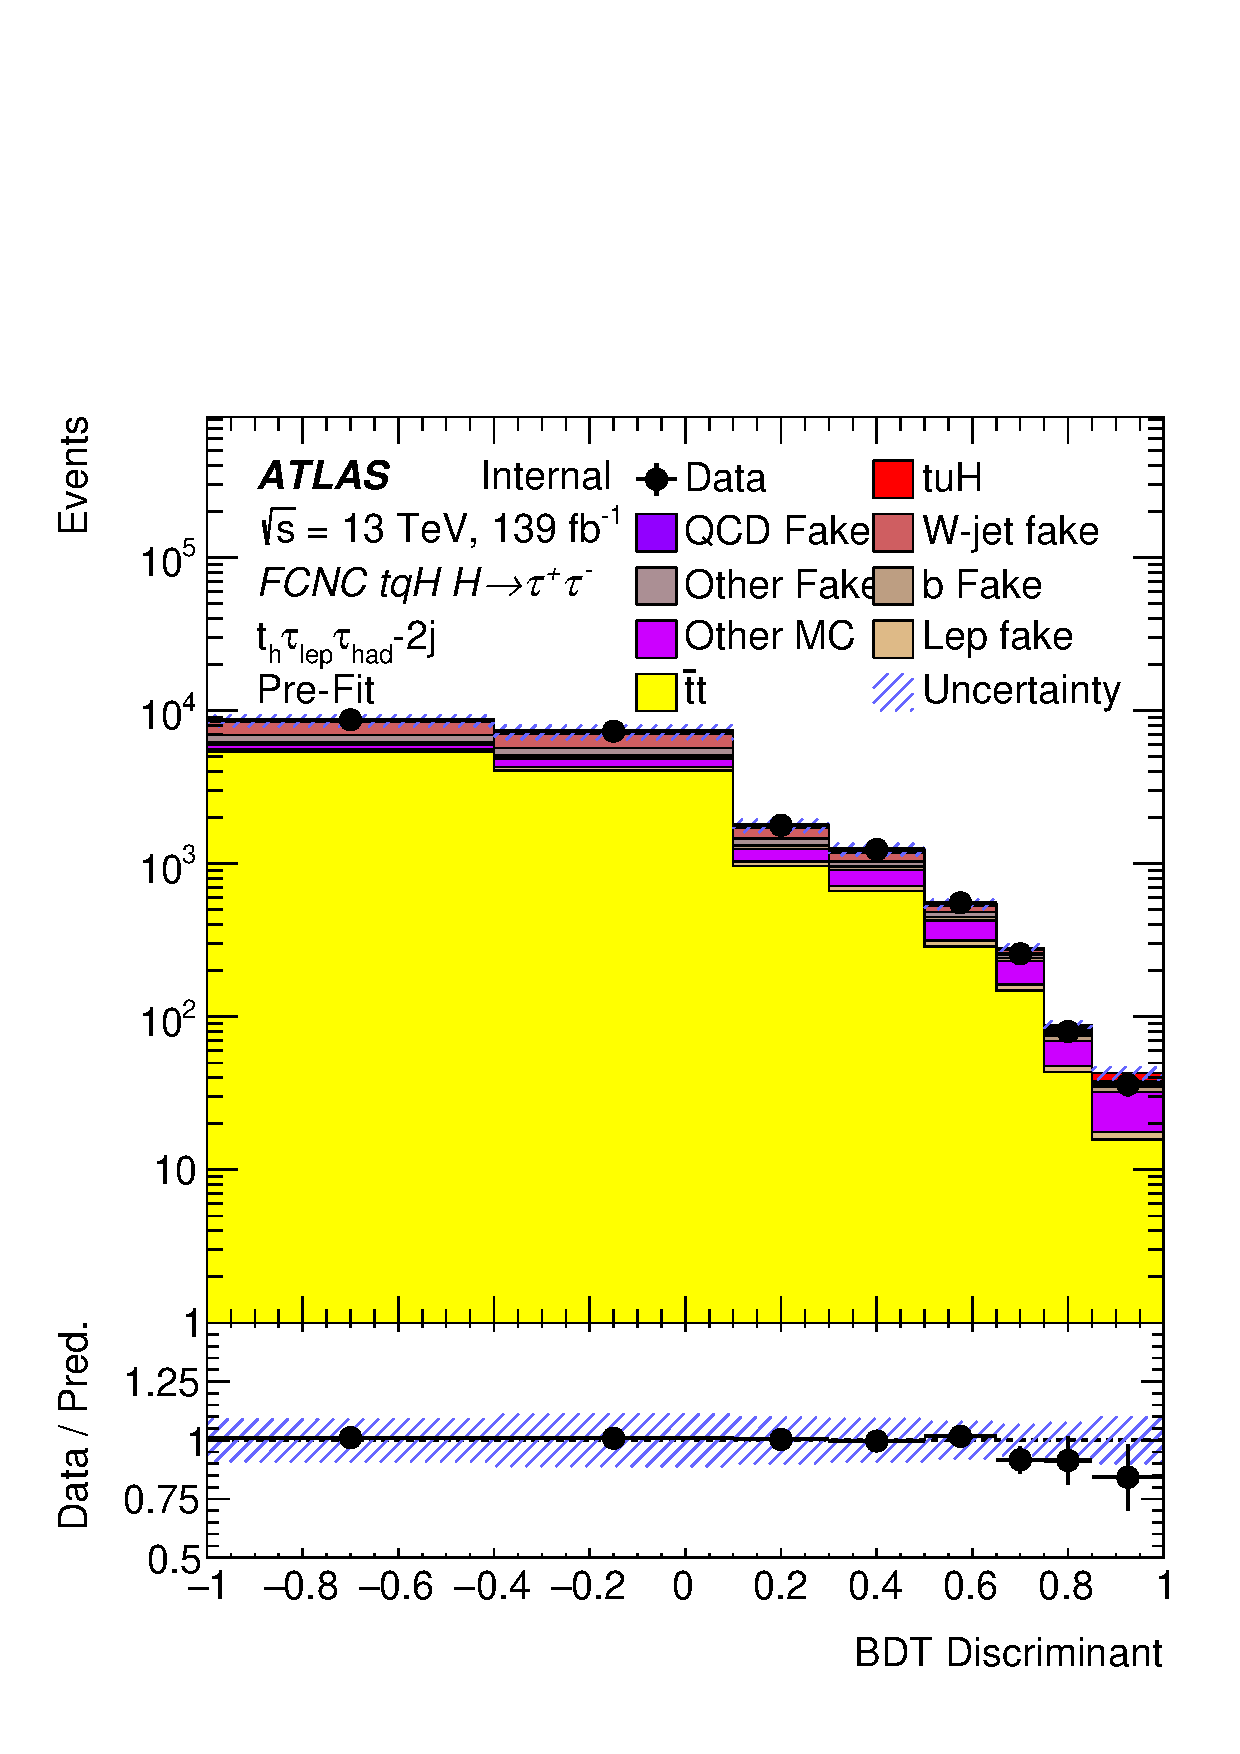
\includegraphics[width=0.25\textwidth]{figures/r21/thq1lntau/ROC/reg1l1tau1b2j_os.pdf}
\put(-70, 70){\textbf{(c3)}}\\
\includegraphics[page=4,width=0.25\textwidth]{figures/r21/thq1lntau/Wfake/doublecount/plots_NOMINAL/reg1l1tau1b3j_os/BDTG_test.pdf}
\put(-30, 80){\textbf{(d1)}}
\includegraphics[page=5,width=0.25\textwidth]{figures/r21/thq1lntau/Wfake/doublecount/plots_NOMINAL/reg1l1tau1b3j_os/BDTG_test.pdf}
\put(-30, 80){\textbf{(d2)}}
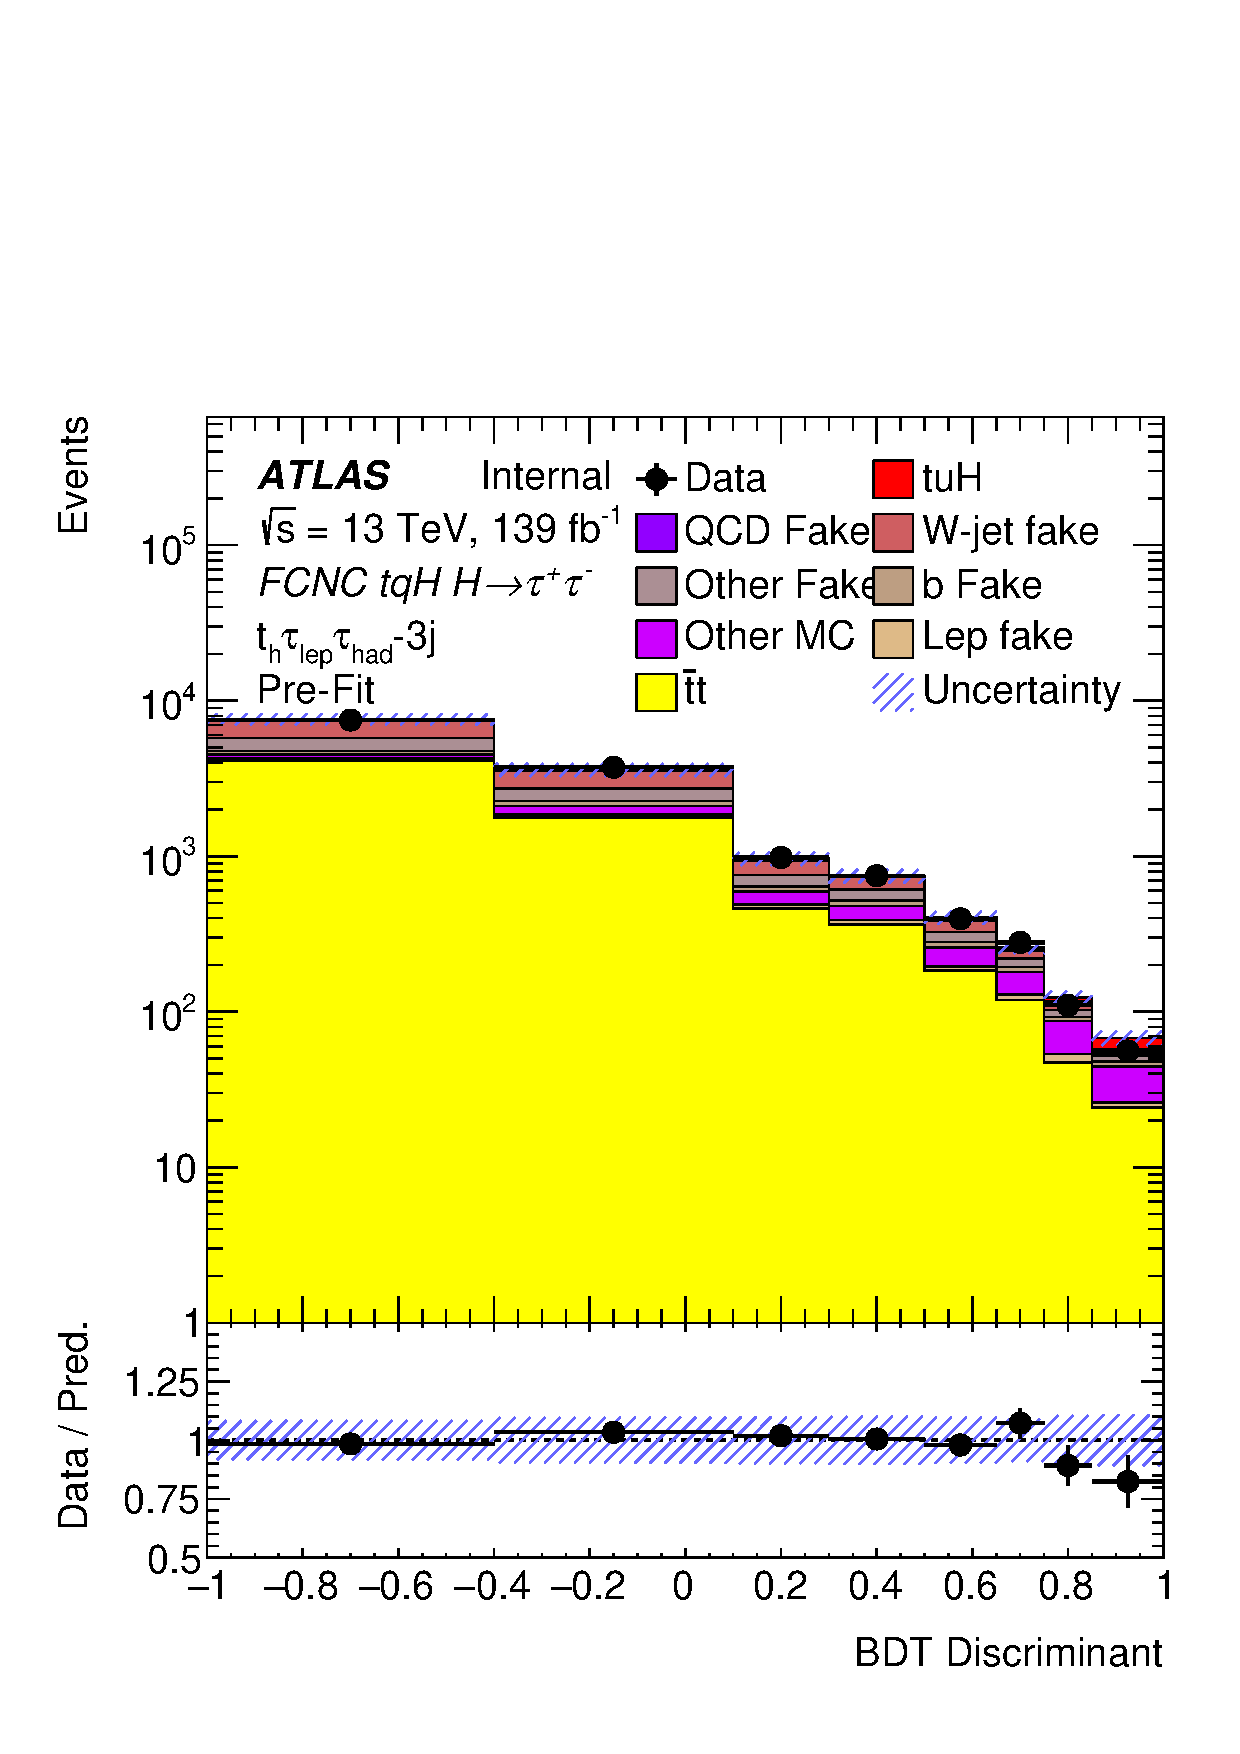
\includegraphics[width=0.25\textwidth]{figures/r21/thq1lntau/ROC/reg1l1tau1b3j_os.pdf}
\put(-70, 70){\textbf{(d3)}}\\
\includegraphics[page=4,width=0.25\textwidth]{figures/r21/thq1lntau/Wfake/doublecount/plots_NOMINAL/reg1l2tau1bnj_os/BDTG_test.pdf}
\put(-30, 80){\textbf{(e1)}}
\includegraphics[page=5,width=0.25\textwidth]{figures/r21/thq1lntau/Wfake/doublecount/plots_NOMINAL/reg1l2tau1bnj_os/BDTG_test.pdf}
\put(-30, 80){\textbf{(e2)}}
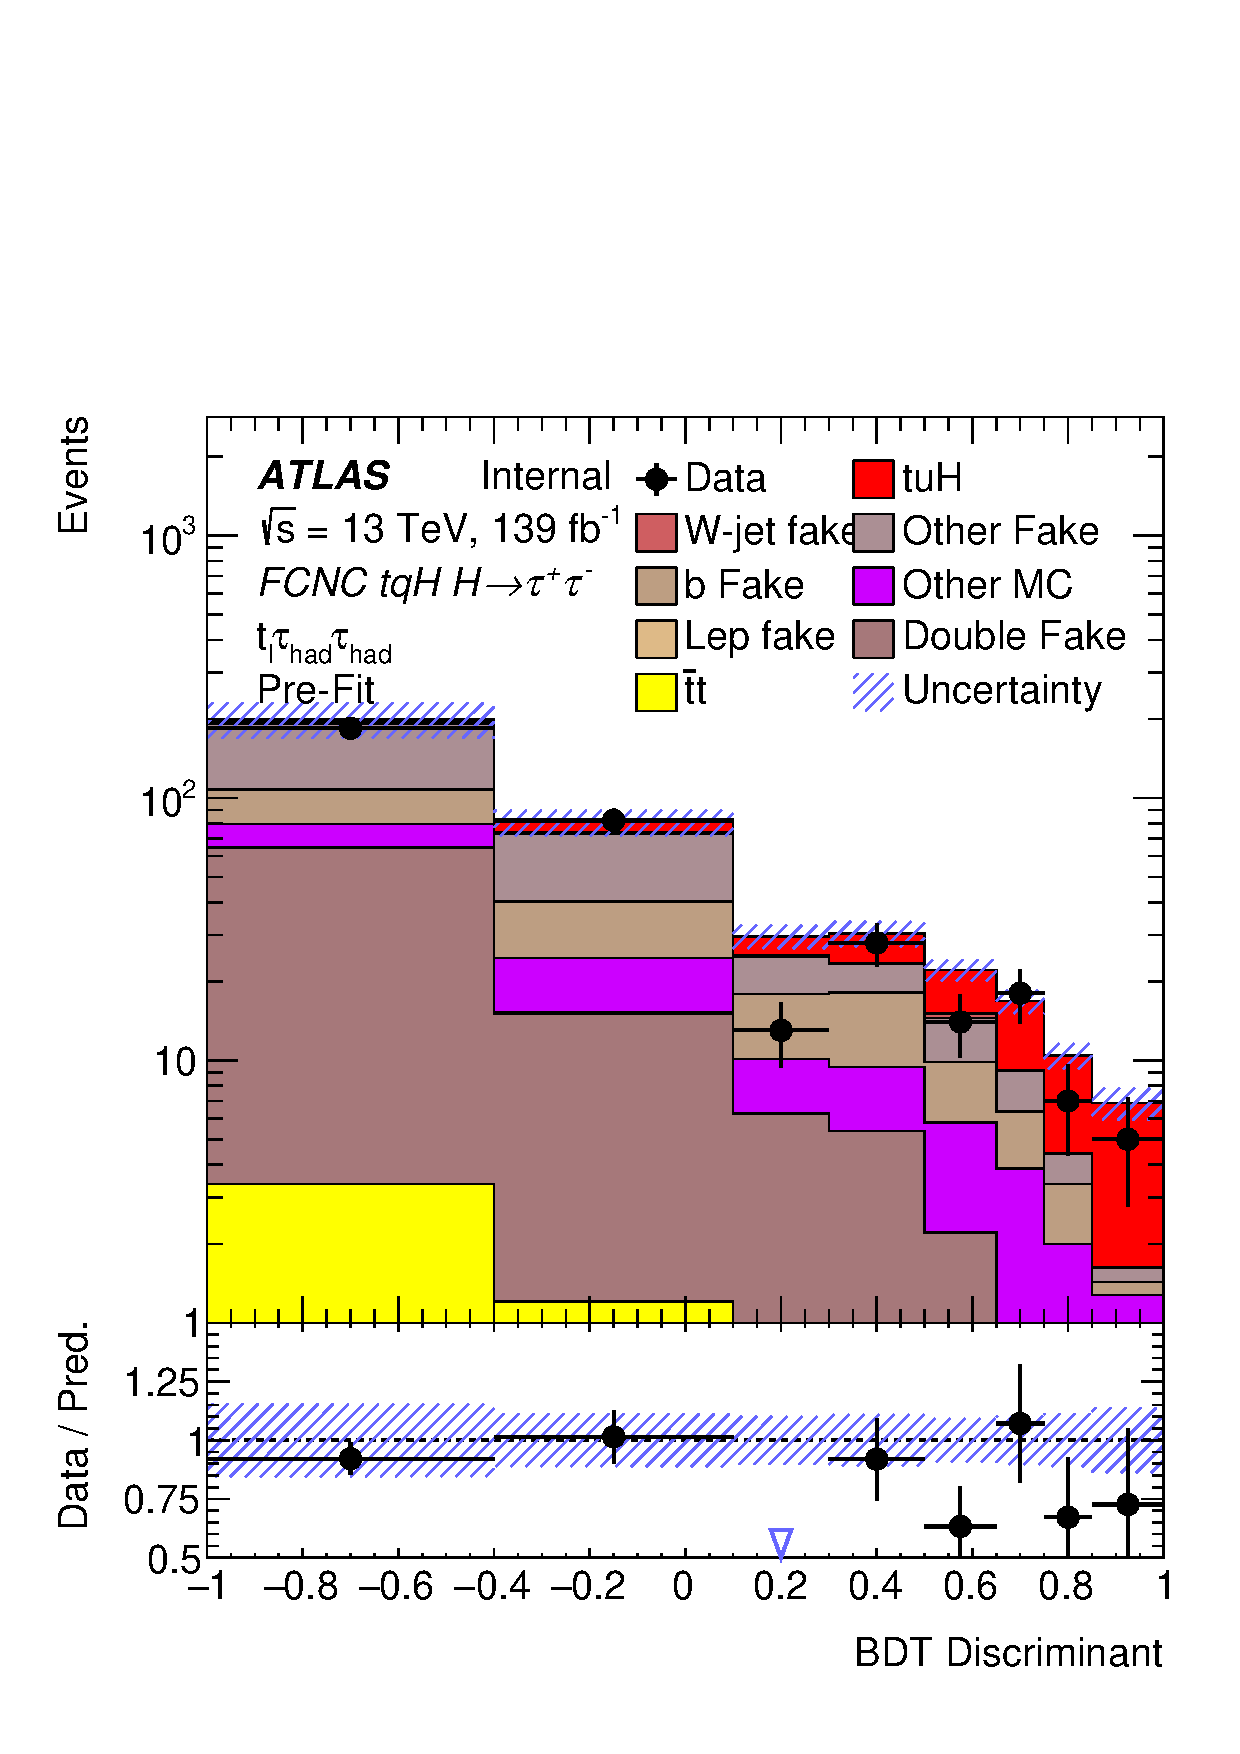
\includegraphics[width=0.25\textwidth]{figures/r21/thq1lntau/ROC/reg1l2tau1bnj_os.pdf}
\put(-70, 70){\textbf{(e3)}}\\
\caption{ The BDT output distributions for the background and TT signal (a1, b1, c1, d1, e1), background and ST signal (a2, b2, c2, d2, e2) and ROC curves (a3, b3, c3, d3, e3) in the STH $\thadhad$ (a1-3), TTH $\thadhad$ (b1-3), STH $\tlhad$ (c1-3), TTH $\tlhad$ (d1-3),  $l\thadhad$ (e1-3) channels. }% The Kolmogorov Test values for the training and testing BDT distributions are also indicated.
\label{fig:overtrain}
\end{figure}

The final yield and stat. only significance is shown in Table \ref{tab:yield} and Table \ref{tab:significance}


\input{tables/hadhad_significance_chart}
\centering
\begin{tabular}{|c|c|c|c|c|} \hline
 & 1l1tau1b1j ss e  highmet & 1l1tau1b1j ss e  lowmet & 1l1tau1b1j ss mu  highmet & 1l1tau1b1j ss mu  lowmet\\\hline
$\bar{t}t\to bWcH$ & $0.61$ & $0.23$ & $1.11$ & $0.34$\\\hline
$cg\to tH$ & $0.02$ & $0.01$ & $0.04$ & $0.01$\\\hline
tcH~merged~signal & $0.63$ & $0.24$ & $1.15$ & $0.35$\\\hline
$\bar{t}t\to bWuH$ & $0.64$ & $0.22$ & $1.18$ & $0.39$\\\hline
$ug\to tH$ & $0.05$ & $0.02$ & $0.28$ & $0.09$\\\hline
tuH~merged~signal & $0.70$ & $0.24$ & $1.45$ & $0.48$\\\hline
\end{tabular}
\begin{tabular}{|c|c|c|c|c|} \hline
 & 1l1tau1b2j os e  highmet & 1l1tau1b2j os e  lowmet & 1l1tau1b2j os mu  highmet & 1l1tau1b2j os mu  lowmet\\\hline
$\bar{t}t\to bWcH$ & $0.35$ & $0.13$ & $0.57$ & $0.25$\\\hline
$cg\to tH$ & $0.04$ & $0.01$ & $0.05$ & $0.01$\\\hline
tcH~merged~signal & $0.38$ & $0.14$ & $0.62$ & $0.27$\\\hline
$\bar{t}t\to bWuH$ & $0.36$ & $0.15$ & $0.60$ & $0.23$\\\hline
$ug\to tH$ & $0.21$ & $0.04$ & $0.35$ & $0.07$\\\hline
tuH~merged~signal & $0.55$ & $0.19$ & $0.92$ & $0.30$\\\hline
\end{tabular}
\begin{tabular}{|c|c|c|c|c|} \hline
 & 1l1tau1b2j ss e  highmet & 1l1tau1b2j ss e  lowmet & 1l1tau1b2j ss mu  highmet & 1l1tau1b2j ss mu  lowmet\\\hline
$\bar{t}t\to bWcH$ & $0.59$ & $0.19$ & $1.07$ & $0.35$\\\hline
$cg\to tH$ & $0.02$ & $0.00$ & $0.03$ & $0.01$\\\hline
tcH~merged~signal & $0.61$ & $0.20$ & $1.10$ & $0.36$\\\hline
$\bar{t}t\to bWuH$ & $0.64$ & $0.23$ & $1.13$ & $0.43$\\\hline
$ug\to tH$ & $0.03$ & $0.01$ & $0.23$ & $0.08$\\\hline
tuH~merged~signal & $0.68$ & $0.24$ & $1.35$ & $0.51$\\\hline
\end{tabular}
\begin{tabular}{|c|c|c|c|c|} \hline
 & 1l1tau1b3j os e  highmet & 1l1tau1b3j os e  lowmet & 1l1tau1b3j os mu  highmet & 1l1tau1b3j os mu  lowmet\\\hline
$\bar{t}t\to bWcH$ & $0.76$ & $0.28$ & $1.18$ & $0.50$\\\hline
$cg\to tH$ & $0.04$ & $0.01$ & $0.05$ & $0.02$\\\hline
tcH~merged~signal & $0.79$ & $0.29$ & $1.23$ & $0.51$\\\hline
$\bar{t}t\to bWuH$ & $0.77$ & $0.34$ & $1.28$ & $0.51$\\\hline
$ug\to tH$ & $0.22$ & $0.04$ & $0.30$ & $0.08$\\\hline
tuH~merged~signal & $0.98$ & $0.38$ & $1.58$ & $0.59$\\\hline
\end{tabular}
\begin{tabular}{|c|c|c|c|c|} \hline
 & 1l1tau1b3j ss e  highmet & 1l1tau1b3j ss e  lowmet & 1l1tau1b3j ss mu  highmet & 1l1tau1b3j ss mu  lowmet\\\hline
$\bar{t}t\to bWcH$ & $0.29$ & $0.09$ & $0.48$ & $0.16$\\\hline
$cg\to tH$ & $0.01$ & $0.00$ & $0.01$ & $0.00$\\\hline
tcH~merged~signal & $0.30$ & $0.09$ & $0.49$ & $0.17$\\\hline
$\bar{t}t\to bWuH$ & $0.31$ & $0.10$ & $0.54$ & $0.18$\\\hline
$ug\to tH$ & $0.03$ & $0.01$ & $0.06$ & $0.02$\\\hline
tuH~merged~signal & $0.33$ & $0.11$ & $0.60$ & $0.20$\\\hline
\end{tabular}
\begin{tabular}{|c|c|c|c|c|} \hline
 & 1l1tau2b1j ss e  highmet & 1l1tau2b1j ss e  lowmet & 1l1tau2b1j ss mu  highmet & 1l1tau2b1j ss mu  lowmet\\\hline
$\bar{t}t\to bWcH$ & $0.12$ & $0.07$ & $0.20$ & $0.06$\\\hline
$cg\to tH$ & $0.00$ & $0.00$ & $0.00$ & $0.00$\\\hline
tcH~merged~signal & $0.12$ & $0.07$ & $0.21$ & $0.06$\\\hline
$\bar{t}t\to bWuH$ & $0.04$ & $0.01$ & $0.08$ & $0.02$\\\hline
$ug\to tH$ & $0.01$ & $0.00$ & $0.02$ & $0.01$\\\hline
tuH~merged~signal & $0.04$ & $0.01$ & $0.10$ & $0.03$\\\hline
\end{tabular}
\begin{tabular}{|c|c|c|c|c|} \hline
 & 1l1tau2b2j os e  highmet & 1l1tau2b2j os e  lowmet & 1l1tau2b2j os mu  highmet & 1l1tau2b2j os mu  lowmet\\\hline
$\bar{t}t\to bWcH$ & $0.10$ & $0.03$ & $0.14$ & $0.07$\\\hline
$cg\to tH$ & $0.00$ & $0.00$ & $0.01$ & $0.00$\\\hline
tcH~merged~signal & $0.10$ & $0.03$ & $0.15$ & $0.07$\\\hline
$\bar{t}t\to bWuH$ & $0.03$ & $0.02$ & $0.07$ & $0.02$\\\hline
$ug\to tH$ & $0.02$ & $0.02$ & $0.03$ & $0.01$\\\hline
tuH~merged~signal & $0.04$ & $0.03$ & $0.10$ & $0.03$\\\hline
\end{tabular}
\begin{tabular}{|c|c|c|c|c|} \hline
 & 1l1tau2b2j ss e  highmet & 1l1tau2b2j ss e  lowmet & 1l1tau2b2j ss mu  highmet & 1l1tau2b2j ss mu  lowmet\\\hline
$\bar{t}t\to bWcH$ & $0.07$ & $0.06$ & $0.14$ & $0.04$\\\hline
$cg\to tH$ & $0.00$ & $0.00$ & $0.00$ & $0.00$\\\hline
tcH~merged~signal & $0.07$ & $0.06$ & $0.14$ & $0.04$\\\hline
$\bar{t}t\to bWuH$ & $0.04$ & $0.01$ & $0.07$ & $0.02$\\\hline
$ug\to tH$ & $0.00$ & $0.00$ & $0.02$ & $0.01$\\\hline
tuH~merged~signal & $0.05$ & $0.01$ & $0.08$ & $0.03$\\\hline
\end{tabular}
\begin{tabular}{|c|c|c|c|c|} \hline
 & 1l1tau2b3j os e  highmet & 1l1tau2b3j os e  lowmet & 1l1tau2b3j os mu  highmet & 1l1tau2b3j os mu  lowmet\\\hline
$\bar{t}t\to bWcH$ & $0.14$ & $0.03$ & $0.20$ & $0.10$\\\hline
$cg\to tH$ & $0.00$ & $0.00$ & $0.00$ & $0.00$\\\hline
tcH~merged~signal & $0.14$ & $0.03$ & $0.21$ & $0.10$\\\hline
$\bar{t}t\to bWuH$ & $0.07$ & $0.03$ & $0.10$ & $0.04$\\\hline
$ug\to tH$ & $0.01$ & $0.00$ & $0.03$ & $0.01$\\\hline
tuH~merged~signal & $0.08$ & $0.03$ & $0.13$ & $0.04$\\\hline
\end{tabular}
\begin{tabular}{|c|c|c|c|c|} \hline
 & 1l1tau2b3j ss e  highmet & 1l1tau2b3j ss e  lowmet & 1l1tau2b3j ss mu  highmet & 1l1tau2b3j ss mu  lowmet\\\hline
$\bar{t}t\to bWcH$ & $0.04$ & $0.01$ & $0.08$ & $0.02$\\\hline
$cg\to tH$ & $0.00$ & $0.00$ & $0.00$ & $0.00$\\\hline
tcH~merged~signal & $0.04$ & $0.01$ & $0.08$ & $0.02$\\\hline
$\bar{t}t\to bWuH$ & $0.03$ &  / & $0.04$ & $0.02$\\\hline
$ug\to tH$ & $0.00$ &  / & $0.01$ & $0.00$\\\hline
tuH~merged~signal & $0.03$ &  / & $0.04$ & $0.02$\\\hline
\end{tabular}
\begin{tabular}{|c|c|c|c|c|} \hline
 & 1l2tau1bnj os e  highmet & 1l2tau1bnj os e  lowmet & 1l2tau1bnj os mu  highmet & 1l2tau1bnj os mu  lowmet\\\hline
$\bar{t}t\to bWcH$ & $3.27$ & $1.47$ & $4.80$ & $2.71$\\\hline
$cg\to tH$ & $0.37$ & $0.12$ & $0.47$ & $0.26$\\\hline
tcH~merged~signal & $3.47$ & $1.55$ & $5.13$ & $2.88$\\\hline
$\bar{t}t\to bWuH$ & $3.55$ & $1.67$ & $5.04$ & $2.89$\\\hline
$ug\to tH$ & $0.65$ & $0.27$ & $2.30$ & $1.28$\\\hline
tuH~merged~signal & $3.92$ & $1.86$ & $6.76$ & $3.80$\\\hline
\end{tabular}
\begin{tabular}{|c|c|c|c|c|} \hline
 & 1l2tau1bnj ss e  highmet & 1l2tau1bnj ss e  lowmet & 1l2tau1bnj ss mu  highmet & 1l2tau1bnj ss mu  lowmet\\\hline
$\bar{t}t\to bWcH$ & $0.13$ & $0.15$ & $0.22$ & $0.14$\\\hline
$cg\to tH$ & $0.01$ & $0.01$ & $0.01$ & $0.01$\\\hline
tcH~merged~signal & $0.14$ & $0.16$ & $0.23$ & $0.14$\\\hline
$\bar{t}t\to bWuH$ & $0.18$ & $0.15$ & $0.24$ & $0.18$\\\hline
$ug\to tH$ & $0.05$ & $0.05$ & $0.07$ & $0.04$\\\hline
tuH~merged~signal & $0.22$ & $0.18$ & $0.31$ & $0.21$\\\hline
\end{tabular}
\begin{tabular}{|c|c|c|c|c|} \hline
 & 1l2tau2bnj os e  highmet & 1l2tau2bnj os e  lowmet & 1l2tau2bnj os mu  highmet & 1l2tau2bnj os mu  lowmet\\\hline
$\bar{t}t\to bWcH$ & $0.50$ & $0.60$ & $0.73$ & $0.38$\\\hline
$cg\to tH$ & $0.01$ & $0.02$ & $0.02$ & $0.01$\\\hline
tcH~merged~signal & $0.51$ & $0.61$ & $0.75$ & $0.39$\\\hline
$\bar{t}t\to bWuH$ & $0.15$ & $0.04$ & $0.18$ & $0.10$\\\hline
$ug\to tH$ & $0.01$ & $0.01$ & $0.07$ & $0.02$\\\hline
tuH~merged~signal & $0.16$ & $0.04$ & $0.25$ & $0.12$\\\hline
\end{tabular}
\begin{tabular}{|c|c|c|c|c|} \hline
 & 1l2tau2bnj ss e  highmet & 1l2tau2bnj ss mu  highmet & 1l2tau2bnj ss mu  lowmet & 1l1tau1b1j ss  highmet\\\hline
$\bar{t}t\to bWcH$ & $0.02$ & $0.03$ &  / & $1.26$\\\hline
$cg\to tH$ & $0.00$ & $0.01$ & $0.00$ & $0.05$\\\hline
tcH~merged~signal & $0.02$ & $0.03$ & $0.00$ & $1.31$\\\hline
$\bar{t}t\to bWuH$ & $0.01$ & $0.01$ &  / & $1.34$\\\hline
$ug\to tH$ &  / & $0.00$ &  / & $0.27$\\\hline
tuH~merged~signal & $0.01$ & $0.01$ &  / & $1.60$\\\hline
\end{tabular}
\begin{tabular}{|c|c|c|c|c|} \hline
 & 1l1tau1b1j ss  lowmet & 1l1tau1b2j os  highmet & 1l1tau1b2j os  lowmet & 1l1tau1b2j ss  highmet\\\hline
$\bar{t}t\to bWcH$ & $0.41$ & $0.67$ & $0.28$ & $1.22$\\\hline
$cg\to tH$ & $0.02$ & $0.06$ & $0.02$ & $0.03$\\\hline
tcH~merged~signal & $0.42$ & $0.73$ & $0.30$ & $1.26$\\\hline
$\bar{t}t\to bWuH$ & $0.45$ & $0.70$ & $0.28$ & $1.30$\\\hline
$ug\to tH$ & $0.09$ & $0.40$ & $0.08$ & $0.21$\\\hline
tuH~merged~signal & $0.53$ & $1.07$ & $0.35$ & $1.50$\\\hline
\end{tabular}
\begin{tabular}{|c|c|c|c|c|} \hline
 & 1l1tau1b2j ss  lowmet & 1l1tau1b3j os  highmet & 1l1tau1b3j os  lowmet & 1l1tau1b3j ss  highmet\\\hline
$\bar{t}t\to bWcH$ & $0.39$ & $1.40$ & $0.57$ & $0.56$\\\hline
$cg\to tH$ & $0.01$ & $0.06$ & $0.02$ & $0.01$\\\hline
tcH~merged~signal & $0.40$ & $1.46$ & $0.59$ & $0.57$\\\hline
$\bar{t}t\to bWuH$ & $0.48$ & $1.50$ & $0.61$ & $0.62$\\\hline
$ug\to tH$ & $0.07$ & $0.37$ & $0.09$ & $0.06$\\\hline
tuH~merged~signal & $0.55$ & $1.85$ & $0.70$ & $0.68$\\\hline
\end{tabular}
\begin{tabular}{|c|c|c|c|c|} \hline
 & 1l1tau1b3j ss  lowmet & 1l1tau2b1j ss  highmet & 1l1tau2b1j ss  lowmet & 1l1tau2b2j os  highmet\\\hline
$\bar{t}t\to bWcH$ & $0.19$ & $0.23$ & $0.08$ & $0.17$\\\hline
$cg\to tH$ & $0.00$ & $0.00$ & $0.00$ & $0.01$\\\hline
tcH~merged~signal & $0.19$ & $0.24$ & $0.08$ & $0.18$\\\hline
$\bar{t}t\to bWuH$ & $0.21$ & $0.09$ & $0.02$ & $0.07$\\\hline
$ug\to tH$ & $0.02$ & $0.02$ & $0.01$ & $0.04$\\\hline
tuH~merged~signal & $0.22$ & $0.11$ & $0.03$ & $0.11$\\\hline
\end{tabular}
\begin{tabular}{|c|c|c|c|c|} \hline
 & 1l1tau2b2j os  lowmet & 1l1tau2b2j ss  highmet & 1l1tau2b2j ss  lowmet & 1l1tau2b3j os  highmet\\\hline
$\bar{t}t\to bWcH$ & $0.07$ & $0.16$ & $0.06$ & $0.25$\\\hline
$cg\to tH$ & $0.00$ & $0.00$ & $0.00$ & $0.00$\\\hline
tcH~merged~signal & $0.07$ & $0.16$ & $0.06$ & $0.25$\\\hline
$\bar{t}t\to bWuH$ & $0.03$ & $0.08$ & $0.02$ & $0.13$\\\hline
$ug\to tH$ & $0.01$ & $0.02$ & $0.01$ & $0.03$\\\hline
tuH~merged~signal & $0.04$ & $0.09$ & $0.03$ & $0.15$\\\hline
\end{tabular}
\begin{tabular}{|c|c|c|c|c|} \hline
 & 1l1tau2b3j os  lowmet & 1l1tau2b3j ss  highmet & 1l1tau2b3j ss  lowmet & 1l2tau1bnj os  highmet\\\hline
$\bar{t}t\to bWcH$ & $0.10$ & $0.09$ & $0.02$ & $5.67$\\\hline
$cg\to tH$ & $0.00$ & $0.00$ & $0.00$ & $0.55$\\\hline
tcH~merged~signal & $0.10$ & $0.09$ & $0.02$ & $6.05$\\\hline
$\bar{t}t\to bWuH$ & $0.04$ & $0.05$ & $0.01$ & $6.01$\\\hline
$ug\to tH$ & $0.00$ & $0.01$ & $0.00$ & $2.33$\\\hline
tuH~merged~signal & $0.05$ & $0.05$ & $0.02$ & $7.71$\\\hline
\end{tabular}
\begin{tabular}{|c|c|c|c|c|} \hline
 & 1l2tau1bnj os  lowmet & 1l2tau1bnj ss  highmet & 1l2tau1bnj ss  lowmet & 1l2tau2bnj os  highmet\\\hline
$\bar{t}t\to bWcH$ & $3.00$ & $0.25$ & $0.19$ & $0.87$\\\hline
$cg\to tH$ & $0.27$ & $0.02$ & $0.01$ & $0.02$\\\hline
tcH~merged~signal & $3.19$ & $0.27$ & $0.19$ & $0.89$\\\hline
$\bar{t}t\to bWuH$ & $3.24$ & $0.29$ & $0.21$ & $0.22$\\\hline
$ug\to tH$ & $1.19$ & $0.09$ & $0.05$ & $0.06$\\\hline
tuH~merged~signal & $4.11$ & $0.37$ & $0.25$ & $0.29$\\\hline
\end{tabular}
\begin{tabular}{|c|c|c|c|c|} \hline
 & 1l2tau2bnj os  lowmet & 1l2tau2bnj ss  highmet & 1l2tau2bnj ss  lowmet & 1l1tau1b1j ss\\\hline
$\bar{t}t\to bWcH$ & $0.44$ & $0.03$ &  / & $1.33$\\\hline
$cg\to tH$ & $0.01$ & $0.00$ & $0.00$ & $0.05$\\\hline
tcH~merged~signal & $0.45$ & $0.03$ & $0.00$ & $1.37$\\\hline
$\bar{t}t\to bWuH$ & $0.10$ & $0.01$ &  / & $1.41$\\\hline
$ug\to tH$ & $0.02$ & $0.00$ &  / & $0.28$\\\hline
tuH~merged~signal & $0.12$ & $0.01$ &  / & $1.69$\\\hline
\end{tabular}
\begin{tabular}{|c|c|c|c|c|} \hline
 & 1l1tau1b2j os & 1l1tau1b2j ss & 1l1tau1b3j os & 1l1tau1b3j ss\\\hline
$\bar{t}t\to bWcH$ & $0.72$ & $1.28$ & $1.50$ & $0.59$\\\hline
$cg\to tH$ & $0.07$ & $0.04$ & $0.07$ & $0.01$\\\hline
tcH~merged~signal & $0.78$ & $1.32$ & $1.57$ & $0.60$\\\hline
$\bar{t}t\to bWuH$ & $0.74$ & $1.38$ & $1.61$ & $0.65$\\\hline
$ug\to tH$ & $0.40$ & $0.22$ & $0.38$ & $0.06$\\\hline
tuH~merged~signal & $1.11$ & $1.59$ & $1.98$ & $0.71$\\\hline
\end{tabular}
\begin{tabular}{|c|c|c|c|} \hline
 & 1l1tau2b1j ss & 1l1tau2b2j os & 1l1tau2b2j ss\\\hline
$\bar{t}t\to bWcH$ & $0.25$ & $0.18$ & $0.17$\\\hline
$cg\to tH$ & $0.00$ & $0.01$ & $0.00$\\\hline
tcH~merged~signal & $0.25$ & $0.19$ & $0.17$\\\hline
$\bar{t}t\to bWuH$ & $0.09$ & $0.08$ & $0.08$\\\hline
$ug\to tH$ & $0.02$ & $0.04$ & $0.02$\\\hline
tuH~merged~signal & $0.11$ & $0.11$ & $0.10$\\\hline
\end{tabular}
\begin{tabular}{|c|c|c|c|} \hline
 & 1l1tau2b3j os & 1l1tau2b3j ss & 1l2tau1bnj os\\\hline
$\bar{t}t\to bWcH$ & $0.26$ & $0.09$ & $6.34$\\\hline
$cg\to tH$ & $0.00$ & $0.00$ & $0.61$\\\hline
tcH~merged~signal & $0.27$ & $0.09$ & $6.77$\\\hline
$\bar{t}t\to bWuH$ & $0.13$ & $0.05$ & $6.74$\\\hline
$ug\to tH$ & $0.03$ & $0.01$ & $2.59$\\\hline
tuH~merged~signal & $0.16$ & $0.05$ & $8.64$\\\hline
\end{tabular}
\begin{tabular}{|c|c|c|c|} \hline
 & 1l2tau1bnj ss & 1l2tau2bnj os & 1l2tau2bnj ss\\\hline
$\bar{t}t\to bWcH$ & $0.30$ & $0.96$ & $0.03$\\\hline
$cg\to tH$ & $0.02$ & $0.02$ & $0.00$\\\hline
tcH~merged~signal & $0.31$ & $0.98$ & $0.03$\\\hline
$\bar{t}t\to bWuH$ & $0.35$ & $0.24$ & $0.01$\\\hline
$ug\to tH$ & $0.09$ & $0.06$ & $0.00$\\\hline
tuH~merged~signal & $0.43$ & $0.30$ & $0.01$\\\hline
\end{tabular}

\input{tables/hadhad_yield_chart}
\begin{table}
\footnotesize
\caption{The sample and data yield before the fit.}
\centering
\begin{tabular}{|c|c|c|c|c|} \hline
 & $l\thadhad$ ss & $l\thadhad$ os & STH $\tlhad$ ss & STH $\tlhad$ os\\\hline
data & $24.00\pm4.90$ & $28.00\pm5.29$ & $468.00\pm21.63$ & $6787.00\pm82.38$\\\hline
background & $28.34\pm1.91$ & $22.52\pm1.73$ & $459.96\pm8.96$ & $7004.75\pm32.28$\\\hline
$\bar{t}t\to bWcH$ & $0.29\pm0.04$ & $7.13\pm0.21$ & $7.05\pm0.20$ & $12.49\pm0.32$\\\hline
$cg\to tH$ & $0.01\pm0.00$ & $0.14\pm0.01$ & $0.15\pm0.01$ & $0.40\pm0.02$\\\hline
tcH~merged~signal & $0.30\pm0.04$ & $7.27\pm0.21$ & $7.20\pm0.20$ & $12.89\pm0.32$\\\hline
$\bar{t}t\to bWuH$ & $0.10\pm0.03$ & $0.84\pm0.07$ & $2.37\pm0.12$ & $3.92\pm0.17$\\\hline
$ug\to tH$ & $0.01\pm0.01$ & $0.23\pm0.03$ & $0.79\pm0.05$ & $1.79\pm0.09$\\\hline
tuH~merged~signal & $0.12\pm0.03$ & $1.07\pm0.08$ & $3.16\pm0.13$ & $5.72\pm0.20$\\\hline
\end{tabular}
\begin{tabular}{|c|c|c|c|c|} \hline
 & TTH $\tlhad$ ss & TTH $\tlhad$ os & $l\thadhad$ 2b ss & $l\thadhad$ 2b os\\\hline
data & $556.00\pm23.58$ & $4147.00\pm64.40$ & $75.00\pm8.66$ & $92.00\pm9.59$\\\hline
background & $511.26\pm9.76$ & $4342.91\pm24.01$ & $89.79\pm3.36$ & $79.48\pm3.09$\\\hline
$\bar{t}t\to bWcH$ & $4.61\pm0.17$ & $14.86\pm0.38$ & $0.22\pm0.04$ & $4.17\pm0.16$\\\hline
$cg\to tH$ & $0.06\pm0.01$ & $0.25\pm0.02$ & $0.00\pm0.00$ & $0.09\pm0.01$\\\hline
tcH~merged~signal & $4.68\pm0.17$ & $15.11\pm0.38$ & $0.23\pm0.04$ & $4.26\pm0.16$\\\hline
$\bar{t}t\to bWuH$ & $1.94\pm0.11$ & $3.97\pm0.18$ & $0.04\pm0.02$ & $0.44\pm0.05$\\\hline
$ug\to tH$ & $0.28\pm0.04$ & $1.11\pm0.08$ & $0.00\pm0.01$ & $0.23\pm0.03$\\\hline
tuH~merged~signal & $2.22\pm0.11$ & $5.08\pm0.20$ & $0.04\pm0.02$ & $0.67\pm0.06$\\\hline
\end{tabular}
\begin{tabular}{|c|c|c|c|c|} \hline
 & STH $\tlhad$ 2b ss & STH $\tlhad$ 2b os & TTH $\tlhad$ 2b ss & TTH $\tlhad$ 2b os\\\hline
data & $739.00\pm27.18$ & $9247.00\pm96.16$ & $622.00\pm24.94$ & $4689.00\pm68.48$\\\hline
background & $815.62\pm10.25$ & $9649.40\pm35.13$ & $575.99\pm8.45$ & $4865.38\pm24.75$\\\hline
$\bar{t}t\to bWcH$ & $1.88\pm0.10$ & $5.36\pm0.23$ & $1.21\pm0.08$ & $4.30\pm0.21$\\\hline
$cg\to tH$ & $0.02\pm0.00$ & $0.12\pm0.01$ & $0.02\pm0.00$ & $0.04\pm0.01$\\\hline
tcH~merged~signal & $1.90\pm0.10$ & $5.47\pm0.23$ & $1.23\pm0.08$ & $4.34\pm0.21$\\\hline
$\bar{t}t\to bWuH$ & $0.70\pm0.06$ & $1.28\pm0.10$ & $0.36\pm0.05$ & $1.09\pm0.10$\\\hline
$ug\to tH$ & $0.12\pm0.02$ & $0.50\pm0.05$ & $0.06\pm0.01$ & $0.27\pm0.04$\\\hline
tuH~merged~signal & $0.81\pm0.07$ & $1.78\pm0.11$ & $0.43\pm0.05$ & $1.36\pm0.10$\\\hline
\end{tabular}
\label{tab:yield}
\end{table}


%-------------------------------------------------------------------------------
\section{Systematic uncertainties}
\label{sec:systematics}
%-------------------------------------------------------------------------------
The signal efficiency and the background estimations are affected by uncertainties associated with the detector simulation, the signal modelling and the data-driven background determination. In the combined fit, these uncertainties recommended by the various ATLAS working groups are called Nuisance Parameters (NP), as opposed to the parameter of interest, the signal strength, which is a scaling factor applied on the total number of signal events.

Any systematic effect on the  overall normalisation or shape of the final BDT distribution in the signal region is considered. In \texttt{TRExFitter} \cite{TRExFitter}, the NP pruning is applied, which means that NPs whose impact are less than a certain threshold are discarded. The lower thresholds to remove a shape systematic and a normalisation systematic from the fit are both $1\%$ in the fit.

%\input{\FCNCTables/NPlist}
%Ztautau theory Xsec
%top theory Xsec

\subsection{Luminosity}
\label{sec:systematic_Luminosity}
The integrated luminosity measurement has an uncertainty of $1.7\%$ for the combined Run-2 data, and it is applied to all simulated event samples including both signal and background.

\subsection{Detector-related uncertainties}
\label{sec:syst_det}

Uncertainties related to the detector effects are included for the signal and backgrounds that are estimated using simulation. These uncertainties are also taken into account for the simulated events that enter the data-driven background estimations. All instrumental systematic uncertainties arising from the reconstruction, identification and energy scale of electrons, muons, taus,($b$-)jets and the soft term of the $\met$ measurement are considered. The effect of the energy scale uncertainties on the objects is propagated to the $\met$ calculation. These systematics include uncertainty associated with:

\begin{itemize}
\item The electron and muon trigger, reconstruction, identification and isolation efficiencies. These are estimated with the tag-and-probe method on the $Z\to ll$, $J/\psi\to ll$ and $W\to l\nu$ events \cite{lep_sys}. There are 5NP for electron(El\_ChargeMisID\_STAT, El\_ChargeMisID\_SYST, El\_Reco, El\_ID\_TightLH, El\_Iso\_FCLoose), 8NP for muon(Mu\_TTVA\_STAT, Mu\_TTVA\_SYST, Mu\_ID\_STAT, Mu\_ID\_SYST, Mu\_ID\_STAT\_LOWPT, Mu\_ID\_SYST\_LOWPT, Mu\_Iso\_SYST, Mu\_Iso\_STAT, Mu\_Iso\_STAT), 1NP for single electron trigger, and 2NP for single muon trigger. 
  We also checked the recommended PLIV scale factors can be applied to the electron and muon from
  tau decays using $Z\rightarrow \tau\tau\rightarrow e\mu$ enriched control sample in App.~\ref{sec:CheckPLIV} and additional $\pm 2\%$ systematic uncertainty
  is assigned for PLIV cut for the tau-lepton in the lepton + $\thad$ channels as ``Tau\_PLIV''.
  
\item Electron energy and muon momentum scales. They are estimated from the early 13 TeV $Z\to ll$ events. For electron energy scales, we used 1 NP for EG\_RESOLUTION\_ALL, and 2 NP for EG\_SCALE\_ALL and EG\_SCALE\_AF2. For muon momentum scales, 1NP MUON\_SCALE is used.
\item Jet energy scale (JES) and resolution (JER). The JES uncertainty is estimated by varying the jet energies according to the uncertainties derived from simulation and in-situ calibration measurements using a model with a reduced set of 43 orthogonal NPs (30 NPs for JES and 13 NPs for full JER) \cite{jet_sys} which has up to 30\% correlation losses, which are assumed to be uncorrelated, and the induced changes can be added in quadrature. The individual scale variations on the jets are parameterised in $\pt$ and $\eta$. The total JES uncertianty is below 5\% for most jets and below 1\% for central jets with pT between 300 GeV and 2 TeV.
The difference between the JER in data and MC is represented by one NP. It is applied on the MC by smearing the jet $\pt$ within the prescribed uncertainty.
JVT is applied in the analysis to select jets from hard-scattered vertices. It was found that different MC generators (and different fragmentation models) lead to efficiency differences of up to $1\%$, and the uncertainty on the efficiency measurement was found to be around $0.5\%$. Two NPs are assigned for the JVT efficiency, one for the central and the other for the forward jets.
\item Calibration of the $\met$. The uncertainties on $\met$ due to systematic shifts in the corrections for leptons and jets are accounted for in a fully correlated way in their evaluation for those physics objects, and are therefore not considered independently here. The systematic uncertainty assigned to the track-based soft term used in the $\met$ definition quantifies the resolution and scale of the soft term measurement by using the balance between hard and soft contributions in $Z\to\mu\mu$ events. These uncertainties are studied using the differences between Monte Carlo generators, using Powheg+Pythia8 as the nominal generator \cite{met_sys}. One NP is assigned for the soft-track scale, and two NPs for the soft-track resolution.
\item Jet flavour tagging systematics. The uncertainties on the $b$-tagging are assessed independently for $b$, $c$ and light-flavour quark jets\cite{btag_sys1}. The efficiencies are measured in data using the methods described in \cite{btag_sys2}-\cite{btag_sys3} with the 2015, 2016, 2017, and 2018 data set. There are 82 NPs assigned for the flavour tagging systematics with 19 NPs for light flavor, 19 for $c$, 44 for $b$.
\item Pileup. The uncertainty on the pileup reweighting is evaluated by varying the pileup scale factors by 1$\sigma$ based on the reweighting of the average interactions per bunch crossing. However, this uncertainty is highly correlated with the luminosity uncertainty and may be an overestimate.
\item Tau object systematics. These include the $\tauhad$ reconstruction, identification and trigger efficiencies, the efficiency for tau-electron overlap removal of true $\tauhad$ and true electrons faking $\tauhad$, and the efficiency for a ``medium'' BDT electron rejection. There are also three NPs that cover the tau energy scale (TES) systematics due to the modeling of the detector geometry (\texttt{TAU\_TES\_DETECTOR}), the measurement in the tag-and-probe analysis (\texttt{TAU\_TES\_INSITU}) and the \texttt{Geant4} shower model (\texttt{TAU\_TES\_MODEL}). They are evaluated based on detailed MC variation study, as well as the Run-2 $Z\to\tau\tau$ data for insitu calibrations of the tau TES and trigger efficiencies, as documented in \cite{tau_sys1} and the dedicated software tools \cite{tau_sys2} recommended by the Tau CP Woking Group \cite{TauCP}.
\end{itemize}

\subsection{Uncertainties on fake background estimations}
\label{sec:syst_datadriven}

Systematic uncertainties on the fake background as described in Sec. \ref{sec:background} are considered in the final fit.
The uncertainties of the fake estimation are correlated among all the leptonic channels and among all the hadronic channels,
respectively, but independent between them.

In the leptonic channels, they are named \texttt{fakeSFNP\_Xp\_ptY\_*} (X=1,3 indicating the number of tracks. Y=0,1,2 indicating the $\pt$ bins.) for tau fakes modelled by MC and \texttt{ABCD*} for QCD lepton fakes modelled by ABCD method.

In the hadronic channels, they are named \texttt{FFNP\_Xprong\_ptbinY\_etabinZ} (X=1,3 indicating the number of tracks. Y=0,1,2 indicating the $\pt$ bin. Z=0,1 indicating the central taus and forward taus.) for the statistical uncertainties of the FFs derived from the W+jets control region. \texttt{FFNP\_OS\_CR} and \texttt{FFNP\_SS\_CR} are one-sided NP for the systematic uncertainties of the FFs derived in the OS and SS control regions respectively. \texttt{``Only $\tau_\mathrm{sub}$ real modelling''} is the uncertainty of the MC modelling of the events with leading tau fake but sub-leading tau real, which is varied by 50\% to be conservative according to the study in the leptonic channels.

\subsection{Theoretical uncertainties on the background}

Theoretical uncertainties have been applied to the MC background in this analysis. The NNPDF3.0 systematic set (which has 100 variations: PDFset=26001-26100) is used to get the variation envelope around the nominal PDF.

The $\alpha_s$ uncertainty is applied using weights PDFset=26600,26500. The impact is insignificant and pruned before the fit.

The renormalization and factorization scales are varied by a factor of 0.5 and 2.0 around the nominal values. There are eight such variations. In the final BDT distributions, the largest variations of the eight per bin are taken. The name of this theoretical NP is called ``scale'' in the final fit.

The ISR and FSR uncertainty are obtained by weights:
\begin{itemize}
	\item FSR up: ``isr:muRfac=10\_fsr:muRfac=05''
	\item FSR down: ``isr:muRfac=10\_fsr:muRfac=05''
	\item ISR up: ``Var3cUp''
	\item ISR down: ``Var3cDown''
\end{itemize}

The theory uncertainty are applied with both shapes and normalisations hence no additional k-factor normalisation uncertainty is applied.

The default $t\bar{t}$ MC events (DSID=410470) are showered with Pythia8. A separate sample showered with Herwig7 (DSID=410557+410558, version 7.0.4) is compared with Pythia8 sample (DSID=410470), and the difference is treated as fragmentation and hadronization systematics \cite{ttbarSys}. These two samples are both simulated with ATLFAST-II \cite{AFII}, and their difference is then applied to the default full-simulation $t\bar{t}$ sample, shown as ``$\bar{t}t$ PS'' in the ranking plots.

%The default $t\bar{t}$ sample is generated with full simulated Powheg. Separate AFII aMC (DSID=410464+410465, version 2.3.3) and Powheg (DSID=411288) samples are generated, both with Matrix Element Correction (MEC) set to off. The difference between those two is treated as the hard scattering systematics \cite{ttbarSys}, shown as ``ME'' in the ranking plots.

The \texttt{hdamp} parameter (which controls the amount of radiation produced by the parton shower in \texttt{POWHEG-BOX v2}) is set to $1.5 m_{\text{top}}$ in the nominal case. Alternative AFII samples are generated with \texttt{hdamp}$=3 m_{\text{top}}$. The difference between it and AFII Powheg Pythia8 sample (DSID=410470) is treated as one of the systematics, named ``$\bar{t}t$ hdamp''.
%The Powheg+Pythia8 $t\bar{t}$ MC is also generated with different shower radiations (initial and final-state radiation modelling). For a sample with increased radiation, the factorisation and renormalization scales are scaled by 0.5 with respect to their nominal values, the \texttt{hdamp} parameter (which controls the amount of radiation produced by the parton shower in \texttt{POWHEG-BOX v2}) is set to $3 m_{\text{top}}$ and the \texttt{A14var3cUp} tune is used. Conversely, for a sample with decreased radiation, the two scales are scaled by 2 with respect to their nominal values, the \texttt{hdamp} is kept at the nominal value of $1.5 m_{\text{top}}$ and the \texttt{A14var3cDown} tune is used \cite{ttbarSys}.

%Uncertainty affecting the normalisation of the $V$+jets and di-boson background is estimated to be about $5\%$ according to the PMG. The uncertainty on single top sross section is $+5\%$/$-4\%$ \cite{WtXsec}\cite{st_uncert_1,st_uncert_2}, on $t\bar{t}V$ $15\%$ \cite{ttV_uncert_1,ttV_uncert_2}, and on $t\bar{t}H$ $+10\%$/$-13\%$ \cite{ttH_uncert}.

Another significancant background stems from the ztautau samples, the following sources of uncertainty are considered for ztautau samples based on the Htautau analysis.
\begin{itemize}
	\item PDF central value: evaluated considering the standarnd deviation of the 100 NNPDF replicas event weights of NNPDF3.0nnlo PDF set used in Sherpa
	\item renormalisation and factorisation scales - $\mu_{R}/\mu_{F}$: evaluated using event-weights provided by Sherpa
	\item ckkw: jet-to-parton matching uncertainty, evaluated using truth-level parameterisation as a function of jet multiplicity and $p_{T}(Z)$
	\item qsf: resummation scale uncertainty, evaluated using truth-level parameterisation as a function of jet multiplicity and and $p_{T}(Z)$
	\item $\alpha_{S}$:evaluated using event-weights provided by Sherpa
	\item PDF alternative value: evalatued comparing predictions from NNPDF3.0nnlo PDF set (nominal) with MMHT2014nnlo68cl and CT14nnlo PDF sets
\end{itemize}

Finally, the other MC samples contribute a very small fraction of background, to be conservative, 20\% variations are assigned to account for the theoretical uncertainties.

\subsection{Uncertainties on the signal modelling}

An additional $1.6\%$ uncertainty on BR($H\to\tau\tau$) (Named as HttBR in the Ranking plots.) is also assigned \cite{HiggsBR} besides the theoretical uncertainties: PDF, $\alpha_s$, ISR, FSR and scale.

In the leptonic channels, the fake tau calibration is also applied to the fake tau part of the signal the same way as the background and treated correlatedly.

The PS uncertainty of the signal is applied by comparing nominal samples (showered with pythia8) with the corresponding Herwig7 samples. The difference is treated as 1$\sigma$ variation.

\section{Fit model and signal extraction}
\label{sec:fit}

The parameter of interest in this search is the signal strength of the FCNC interactions, BR($t\to Hq$) and corresponding production mode cross section. The statistical analysis of the data employs a binned likelihood function constructed as the product of Poisson probability terms, in bins of the BDT output.

To take into account the systematic uncertianties associated with the MC estimation from different sources for both the signal and background samples, the fit model incorporates these systematics as extra Gaussian or Log-Normal constraint terms multiplied with the combined likelihood. The fitted central values and errors of the systematics parameters, or NPs, are expected to follow a normal distribution centered around 0 with unit width, when the Asimov data is used. The fit model construction is obtained with the \texttt{RooFit} and \texttt{RooStats} software, and the model configuration and persistence files (as input to \texttt{RooStats}) are produced by \texttt{TRExFitter} \cite{TRExFitter}, which is a software package interface with \texttt{HistFactory}. The \texttt{TRExFitter} includes additional features such as histogram smoothing, NP pruning (as shown in Figure \ref{fig:xTFW_pruning_0}-\ref{fig:tthML_pruning_2}) and error symmetrization before the fits.
%A procedure called local symmetrization to the systematic variational histograms is implemented to semmetrize bins with one-sided variations which may cause problems in the fit.

The correlated bin-by-bin histogram variation corresponds to the up and down variation of each NP. The independent bin-by-bin fluctuations in the combined MC templates are also treated as NPs. They are incorporated in the model as extra Poisson constraint terms, and are expected to have a fitted value of 1 and a fitted error reflecting the relative statistical error in each particular bin. There is one parameter of interest (POI) freely floating in the fit without any constraints, namely, the signal strength $\mu$ (\texttt{SigXsecOverSM}) which is a multiplicative factor on a presumed branching ratio of BR($t\to Hq$)=$0.1\%$ in this analysis. The errors associated with the different systematics will be properly propagated to the fitted error of $\mu$ in a simultaneous fit of multiple regions via a profiled likelihood scan by the minimization program \texttt{MINUIT}. 

The one-sided NPs in the analysis, namely, \texttt{fakeSFXprongXPtbin}, \texttt{``ttbar fragmentation''}, \texttt{``ttbar hard scattering''}, \texttt{JET$\_$BJES$\_$Response}, \texttt{JET$\_$JER$\_$DataVsMC$\_$MC16}, \texttt{JET$\_$SingleParticle$\_$HighPt}, \texttt{JET$\_$TILECORR$\_$Uncertainty}, \texttt{MET$\_$SoftTrk$\_$ResoPara}, \texttt{MET$\_$SoftTrk$\_$ResoPerp} are symmetrized. This is done manually on the MC components of the background. By default, all the kinematic NPs (shape NPs due to, e.g., energy scales) are smoothed using the default smoothing parameters (set to 40) in \texttt{TRExFitter}. This helps removing the artificial NP constraints due to statistical fluctuations in the systematic variations, and makes the fit well behaved. %The NPs pull distributions before the smoothing for each SR are given in App. \ref{app:channel_fit}.

Figure~\ref{fig:fcnc_rank_data} shows the ranking of the 30 top NPs along with their pull distributions, produced also with {\texttt TRExFitter}. The highest ranked NP is defined to have the largest impact on $\mu$. The impact is evaluated by varying the NP under consideration by one $\sigma$ (either pre or post-fit error) up and down, and afterwards looking at the relative change in $\mu$ under the conditional fit where the NP under consideration is fixed to its varied new value.
Figure~\ref{fig:fcnc_pull_data} shows the pull distributions of all NPs in asimov fit. %The NPs which are constrained less than $80\%$ of their original error are smoothed with the default smoothing method in {\texttt TRExFitter}. The pre and post-smoothing distributions of the relevant NPs are given in App. \ref{app:smoothpruneNP}. Similar pull distributions before the NP smoothing are given in Figure \ref{fig:fcnc_pull_nosmooth} of App. \ref{app:smoothpruneNP}.
Normalization and shape systematics whose impact is less than $1\%$ are removed from the fit. %The list of removed NPs are given in App. \ref{app:smoothpruneNP}.

It is observed that the NP ``$\bar{t}t$ PS'' is highly constrained. The reason for this is further understood. As shown in App. \ref{sec:decor} in Figure \ref{fig:tuH_NuisPar_decorr} (left), the constraint is originated from signal regions with high statistics especially $t_h\tlhad 3j$. The NP impact on the background is shown in Figure \ref{fig:tthML_ttbarPS}. It is clear that the NP variation is around 2.5\% which is quite significant compared to the statistical uncertainty in the low BDT region. By inspecting the correlation matrix, the NP ``$\bar{t}t$ PS'' doesn't have correlation with other NPs significant enough to be released.

As shown in the plot on the right in Figure \ref{fig:tuH_NuisPar_decorr}. The constraint is mainly caused by the variation of ``$\bar{t}t$'' events with real taus.
This comes from the difference of the samples themselves and has nothing to do with the fake tau background estimation. The constraint is a little bit released in the $t_h\tlhad 3j$ region on the right plot. It is observed that the PS variation also has large impact in the $t\bar{t}$ CR, further more, this NP is also an issue in the FCNC $H\to \bar{b}b$ analysis.

% these questions are too confusing here and we need to check with experts for sure if they see any difference between pythia8 vs herwig7.1, commented for now. 

%So the question on the PS variation is translated to the questions to the $t\bar{t}$ MC analyses:
%\begin{itemize}
%	\item Why are those two samples so different?
%	\item Should the two AFII samples be calibrated separately?
%	\item Is this difference also observed in the studies on the top physics? If so, how is the constraint released?
%	\item Are the taus treated similarly in Herwig7 samples and Pythia8 samples?
%\end{itemize}

%The NP ranking and constraints can be qualitatively understood from the variations of the BDT distributions due to the relevant NPs. Figures \ref{fig:NPvar_rank_data_a}-\ref{fig:NPvar_rank_data_d} show the systematic variations due to the top ranked NPs. %All of them cause large variations in the high-BDT signal region, hence are ranked high. The \texttt{THEORY\_RADIATION} is also constrained to $<80\%$ due to bins where the systematic variation is much bigger than the statistical one. However, after smoothing, this NP is not constrained any more. 

%The latter two cause large variation in the signal region, but small variation in the low BDT background region. Thus, they have large impact on the fitted signal strength but are not much constrained by the fit. The first one causes large variations in the background region, but it is an overall shift effect which can be adjusted by the fit through the floating normalization factors of the fake. Therefore, this NP is not constrained either. The \texttt{NOS\_TOPFRAC\_LH} only affects the $\tlhad$ channel, so the variation in hadronic is null. It causes up to $10\%$ bin-by-bin variations in both the signal and the background regions, which explains why it has a high ranking and is constrained at the same time.
%Figure \ref{fig:NPvar_other} shows the systematic variations due to a few constrained NPs, \texttt{JET\_JES\_PILEUP\_RHOTOPOLOGY}, \texttt{TAU\_TES\_INSITU} and \texttt{MET\_SOFTTRK\_RESOPERP}. They cause about $5-20\%$ bin-by-bin variations in the low BDT region, which can be constrained by the background region events. As a result, their impact on the signal is also reduced. Note that \texttt{MET\_SOFTTRK\_RESOPERP} is a one-sided NP, whose upward and downward variations are set to be the same.

Figure~\ref{fig:fcnc_correl_data_1}-\ref{fig:fcnc_correl_data_2}shows the correlation matrix for diffrent NPs. Except for self-correlations, and the correlations between FSR and Btag\_B\_0 with 27\%, FSR with TAU\_PLIV at -44.9\%, JET\_Flavour\_Composition with JET\_Pileup\_RhoTopology at -34.8\%,   
FSR with scale at 14.4\%, and Fakes from ABCD for electron and muon at -60\%, all other NPs have relatively small correlations with each other in the leptonic channels, which justifies the fit models for independent systematics. These high correlations are due to the fact that the FSR has significant impact on the low b-jet pT as well as the yields of selected
$t\bar t$ events; Similarly, the number of electron and muon fakes are constrains by the sum in the fit.   

\input{\FCNCFigures/tex/tthML_trexPrefit}
\input{\FCNCFigures/tex/xTFW_trexPrefit}

\begin{figure}[htb]
\centering
\includegraphics[width=0.25\textwidth]{\FCNCFigures/xTFW/Limit/tuH_NuisPar.pdf}
\includegraphics[width=0.25\textwidth]{\FCNCFigures/tthML/Limit/tuH_NuisPar.pdf}
\caption{ The pull distributions of asimov fit in hadronic channels (left) combined and leptonic channels combined (right) in terms of tuH merged signal . }
\label{fig:fcnc_pull_data}
\end{figure}


\begin{figure}[htb]
\centering
\includegraphics[width=0.4\textwidth]{\FCNCFigures/xTFW/Limit/tuH_Pruning_0.pdf}
\includegraphics[width=0.4\textwidth]{\FCNCFigures/xTFW/Limit/tuH_Pruning_1.pdf}
\caption{ Summary of the pruned nuisance parameters in the fit to the  Asimov dataset under the S+B hypothesis in hadronic channels part 1 in terms of tuH merged signal. The systematic uncertainties that did not survive the pruning are indicated in red. Green corresponds to the uncertainties for which both shape and normalisation is kept, yellow(orange) indicates that shape (normalisation) is kept. Grey indicates that the uncertainty is not present.}
\label{fig:xTFW_pruning_0}
\end{figure}

\begin{figure}[htb]
\centering
\includegraphics[width=0.6\textwidth]{\FCNCFigures/xTFW/Limit/tuH_Pruning_2.pdf}
\caption{ Summary of the pruned nuisance parameters in the fit to the Asimov dataset under the S+B hypothesis in hadronic channels part 2 in terms of tuH merged signal. The systematic uncertainties that did not survive the pruning are indicated in red. Green corresponds to the uncertainties for which both shape and normalisation is kept, yellow(orange) indicates that shape (normalisation) is kept. Grey indicates that the uncertainty is not present.}
\label{fig:xTFW_pruning_1}
\end{figure}


\begin{figure}[htb]
\centering
\includegraphics[width=0.99\textwidth]{\FCNCFigures/tthML/Limit/tuH_Pruning_0.pdf}
\caption{ Summary of the pruned nuisance parameters in the fit to the  Asimov dataset under the S+B hypothesis in leptonic channels part 1 in terms of tuH merged signal. The systematic uncertainties that did not survive the pruning are indicated in red. Green corresponds to the uncertainties for which both shape and normalisation is kept, yellow(orange) indicates that shape (normalisation) is kept. Grey indicates that the uncertainty is not present.}
\label{fig:tthML_pruning_0}
\end{figure}

\begin{figure}[htb]
\centering
\includegraphics[width=0.99\textwidth]{\FCNCFigures/tthML/Limit/tuH_Pruning_1.pdf}
\caption{ Summary of the pruned nuisance parameters in the fit to the  Asimov dataset under the S+B hypothesis in leptonic channels part 2 in terms of tuH merged signal. The systematic uncertainties that did not survive the pruning are indicated in red. Green corresponds to the uncertainties for which both shape and normalisation is kept, yellow(orange) indicates that shape (normalisation) is kept. Grey indicates that the uncertainty is not present. }
\label{fig:tthML_pruning_1}
\end{figure}

\begin{figure}[htb]
\centering
\includegraphics[width=0.99\textwidth]{\FCNCFigures/tthML/Limit/tuH_Pruning_2.pdf}
\caption{ Summary of the pruned nuisance parameters in the fit to the  Asimov dataset under the S+B hypothesis in leptonic channels part 3 in terms of tuH merged signal. The systematic uncertainties that did not survive the pruning are indicated in red. Green corresponds to the uncertainties for which both shape and normalisation is kept, yellow(orange) indicates that shape (normalisation) is kept. Grey indicates that the uncertainty is not present.}
\label{fig:tthML_pruning_2}
\end{figure}

\begin{figure}[htb]
\centering
\includegraphics[width=0.45\textwidth]{\FCNCFigures/xTFW/Limit/tuH_Ranking.pdf}
\includegraphics[width=0.45\textwidth]{\FCNCFigures/tthML/Limit/tuH_Ranking.pdf}
\caption{ Ranking plot from a fit to a signal-plus-background Asimov dataset for (left) hadronic channels and (right)
leptonic channels in terms of tuH merged signal. All two sided NPs ( with up and down) are symmetrized by "TWOSIDED" and one sided NPs (PS, hdamp, MET, fake estimation etc.) are symmetrized by "ONESIDED". The fitted values of the most important nuisance parameters and their impact on the measured
signal strength are shown. The black points, which are plotted according to the bottom horizontal scale, show the deviation
of each of the fitted nuisance parameters,$\hat{\theta}$, from $\theta_{0}$, which is the nominal value of that nuisance parameter, in units of the
pre-fit standard deviation $\Delta\theta$. The black error bars show the post-fit errors, $\sigma_{\theta}$ , which are close to 1 if these data do not
provide any further constraint on that uncertainty. Conversely, a value of $\sigma_{\theta}$ much smaller than 1 indicates a significant
reduction with respect to the original uncertainty. The nuisance parameters are sorted according to the post-fit effect of each on $\mu$ (hashed blue area),
with those with the largest impact at the top. The scale NP is for a variation of normalization and factorization. Only the leading 30 nuisance parameters are shown. The post-fit effect on $\mu$,
shown according to the top horizontal scale, is calculated by fixing the corresponding nuisance parameter at $\hat{\theta}\pm \sigma_{\theta}$ and
redoing the fit. The difference between the default and modified $\mu$, $\Delta\mu$, represents the effect of the systematic uncertainty
in question on $\mu$.}
\label{fig:fcnc_rank_data}
\end{figure}

\begin{figure}[htb]
\centering
\includegraphics[width=0.45\textwidth]{\FCNCFigures/xTFW/Limit/tcH_Ranking.pdf}
\includegraphics[width=0.45\textwidth]{\FCNCFigures/tthML/Limit/tcH_Ranking.pdf}
\caption{ Ranking plot from a fit to a signal-plus-background Asimov dataset for (left) hadronic channels and (right)
leptonic channels in terms of tcH merged signal. All two sided NPs ( with up and down) are symmetrized by "TWOSIDED" and one sided NPs (PS, hdamp, MET, fake estimation etc.) are symmetrized by "ONESIDED". The fitted values of the most important nuisance parameters and their impact on the measured
signal strength are shown. The black points, which are plotted according to the bottom horizontal scale, show the deviation
of each of the fitted nuisance parameters,$\hat{\theta}$, from $\theta_{0}$, which is the nominal value of that nuisance parameter, in units of the
pre-fit standard deviation $\Delta\theta$. The black error bars show the post-fit errors, $\sigma_{\theta}$ , which are close to 1 if these data do not
provide any further constraint on that uncertainty. Conversely, a value of $\sigma_{\theta}$ much smaller than 1 indicates a significant
reduction with respect to the original uncertainty. The nuisance parameters are sorted according to the post-fit effect of each on $\mu$ (hashed blue area),
with those with the largest impact at the top. The scale NP is for a variation of normalization and factorization. Only the leading 30 nuisance parameters are shown. The post-fit effect on $\mu$,
shown according to the top horizontal scale, is calculated by fixing the corresponding nuisance parameter at $\hat{\theta}\pm \sigma_{\theta}$ and
redoing the fit. The difference between the default and modified $\mu$, $\Delta\mu$, represents the effect of the systematic uncertainty
in question on $\mu$.}
\label{fig:fcnc_rank_data_tcH}
\end{figure}


\begin{figure}[htb]
\centering
\includegraphics[width=1\textwidth]{\FCNCFigures/xTFW/Limit/tuH_CorrMatrix.pdf}
\caption{ Correlation matrix corresponding to the fit to the Asimov dataset under the signal-plus-background hypothesis. Only nuisance parameters with a correlation coefficient of at least 1\% with any other parameter are displayed for hadronic channels combined.}
\label{fig:fcnc_correl_data_1}
\end{figure}


\begin{figure}[htb]
\centering
\includegraphics[width=1\textwidth]{\FCNCFigures/tthML/Limit/tuH_CorrMatrix.pdf}
\caption{ Correlation matrix corresponding to the fit to the Asimov dataset under the signal-plus-background hypothesis. Only nuisance parameters with a correlation coefficient of at least 1\% with any other parameter are displayed for leptonic channels combined.}
\label{fig:fcnc_correl_data_2}
\end{figure}












\section{Results}
\label{sec:results}

The statistical only significance based on BDT discriminant is shown in Table \ref{tab:tthML_significance}, \ref{tab:xTFW_significance}.

\begin{table}
\caption{The statistical only significance in leptonic channels based on BDT discriminant.}
\label{tab:tthML_significance}
\centering
\begin{tabular}{|c|c|c|c|c|} \hline
 & 1l1tau1b1j ss e  highmet & 1l1tau1b1j ss e  lowmet & 1l1tau1b1j ss mu  highmet & 1l1tau1b1j ss mu  lowmet\\\hline
$\bar{t}t\to bWcH$ & $0.61$ & $0.23$ & $1.11$ & $0.34$\\\hline
$cg\to tH$ & $0.02$ & $0.01$ & $0.04$ & $0.01$\\\hline
tcH~merged~signal & $0.63$ & $0.24$ & $1.15$ & $0.35$\\\hline
$\bar{t}t\to bWuH$ & $0.64$ & $0.22$ & $1.18$ & $0.39$\\\hline
$ug\to tH$ & $0.05$ & $0.02$ & $0.28$ & $0.09$\\\hline
tuH~merged~signal & $0.70$ & $0.24$ & $1.45$ & $0.48$\\\hline
\end{tabular}
\begin{tabular}{|c|c|c|c|c|} \hline
 & 1l1tau1b2j os e  highmet & 1l1tau1b2j os e  lowmet & 1l1tau1b2j os mu  highmet & 1l1tau1b2j os mu  lowmet\\\hline
$\bar{t}t\to bWcH$ & $0.35$ & $0.13$ & $0.57$ & $0.25$\\\hline
$cg\to tH$ & $0.04$ & $0.01$ & $0.05$ & $0.01$\\\hline
tcH~merged~signal & $0.38$ & $0.14$ & $0.62$ & $0.27$\\\hline
$\bar{t}t\to bWuH$ & $0.36$ & $0.15$ & $0.60$ & $0.23$\\\hline
$ug\to tH$ & $0.21$ & $0.04$ & $0.35$ & $0.07$\\\hline
tuH~merged~signal & $0.55$ & $0.19$ & $0.92$ & $0.30$\\\hline
\end{tabular}
\begin{tabular}{|c|c|c|c|c|} \hline
 & 1l1tau1b2j ss e  highmet & 1l1tau1b2j ss e  lowmet & 1l1tau1b2j ss mu  highmet & 1l1tau1b2j ss mu  lowmet\\\hline
$\bar{t}t\to bWcH$ & $0.59$ & $0.19$ & $1.07$ & $0.35$\\\hline
$cg\to tH$ & $0.02$ & $0.00$ & $0.03$ & $0.01$\\\hline
tcH~merged~signal & $0.61$ & $0.20$ & $1.10$ & $0.36$\\\hline
$\bar{t}t\to bWuH$ & $0.64$ & $0.23$ & $1.13$ & $0.43$\\\hline
$ug\to tH$ & $0.03$ & $0.01$ & $0.23$ & $0.08$\\\hline
tuH~merged~signal & $0.68$ & $0.24$ & $1.35$ & $0.51$\\\hline
\end{tabular}
\begin{tabular}{|c|c|c|c|c|} \hline
 & 1l1tau1b3j os e  highmet & 1l1tau1b3j os e  lowmet & 1l1tau1b3j os mu  highmet & 1l1tau1b3j os mu  lowmet\\\hline
$\bar{t}t\to bWcH$ & $0.76$ & $0.28$ & $1.18$ & $0.50$\\\hline
$cg\to tH$ & $0.04$ & $0.01$ & $0.05$ & $0.02$\\\hline
tcH~merged~signal & $0.79$ & $0.29$ & $1.23$ & $0.51$\\\hline
$\bar{t}t\to bWuH$ & $0.77$ & $0.34$ & $1.28$ & $0.51$\\\hline
$ug\to tH$ & $0.22$ & $0.04$ & $0.30$ & $0.08$\\\hline
tuH~merged~signal & $0.98$ & $0.38$ & $1.58$ & $0.59$\\\hline
\end{tabular}
\begin{tabular}{|c|c|c|c|c|} \hline
 & 1l1tau1b3j ss e  highmet & 1l1tau1b3j ss e  lowmet & 1l1tau1b3j ss mu  highmet & 1l1tau1b3j ss mu  lowmet\\\hline
$\bar{t}t\to bWcH$ & $0.29$ & $0.09$ & $0.48$ & $0.16$\\\hline
$cg\to tH$ & $0.01$ & $0.00$ & $0.01$ & $0.00$\\\hline
tcH~merged~signal & $0.30$ & $0.09$ & $0.49$ & $0.17$\\\hline
$\bar{t}t\to bWuH$ & $0.31$ & $0.10$ & $0.54$ & $0.18$\\\hline
$ug\to tH$ & $0.03$ & $0.01$ & $0.06$ & $0.02$\\\hline
tuH~merged~signal & $0.33$ & $0.11$ & $0.60$ & $0.20$\\\hline
\end{tabular}
\begin{tabular}{|c|c|c|c|c|} \hline
 & 1l1tau2b1j ss e  highmet & 1l1tau2b1j ss e  lowmet & 1l1tau2b1j ss mu  highmet & 1l1tau2b1j ss mu  lowmet\\\hline
$\bar{t}t\to bWcH$ & $0.12$ & $0.07$ & $0.20$ & $0.06$\\\hline
$cg\to tH$ & $0.00$ & $0.00$ & $0.00$ & $0.00$\\\hline
tcH~merged~signal & $0.12$ & $0.07$ & $0.21$ & $0.06$\\\hline
$\bar{t}t\to bWuH$ & $0.04$ & $0.01$ & $0.08$ & $0.02$\\\hline
$ug\to tH$ & $0.01$ & $0.00$ & $0.02$ & $0.01$\\\hline
tuH~merged~signal & $0.04$ & $0.01$ & $0.10$ & $0.03$\\\hline
\end{tabular}
\begin{tabular}{|c|c|c|c|c|} \hline
 & 1l1tau2b2j os e  highmet & 1l1tau2b2j os e  lowmet & 1l1tau2b2j os mu  highmet & 1l1tau2b2j os mu  lowmet\\\hline
$\bar{t}t\to bWcH$ & $0.10$ & $0.03$ & $0.14$ & $0.07$\\\hline
$cg\to tH$ & $0.00$ & $0.00$ & $0.01$ & $0.00$\\\hline
tcH~merged~signal & $0.10$ & $0.03$ & $0.15$ & $0.07$\\\hline
$\bar{t}t\to bWuH$ & $0.03$ & $0.02$ & $0.07$ & $0.02$\\\hline
$ug\to tH$ & $0.02$ & $0.02$ & $0.03$ & $0.01$\\\hline
tuH~merged~signal & $0.04$ & $0.03$ & $0.10$ & $0.03$\\\hline
\end{tabular}
\begin{tabular}{|c|c|c|c|c|} \hline
 & 1l1tau2b2j ss e  highmet & 1l1tau2b2j ss e  lowmet & 1l1tau2b2j ss mu  highmet & 1l1tau2b2j ss mu  lowmet\\\hline
$\bar{t}t\to bWcH$ & $0.07$ & $0.06$ & $0.14$ & $0.04$\\\hline
$cg\to tH$ & $0.00$ & $0.00$ & $0.00$ & $0.00$\\\hline
tcH~merged~signal & $0.07$ & $0.06$ & $0.14$ & $0.04$\\\hline
$\bar{t}t\to bWuH$ & $0.04$ & $0.01$ & $0.07$ & $0.02$\\\hline
$ug\to tH$ & $0.00$ & $0.00$ & $0.02$ & $0.01$\\\hline
tuH~merged~signal & $0.05$ & $0.01$ & $0.08$ & $0.03$\\\hline
\end{tabular}
\begin{tabular}{|c|c|c|c|c|} \hline
 & 1l1tau2b3j os e  highmet & 1l1tau2b3j os e  lowmet & 1l1tau2b3j os mu  highmet & 1l1tau2b3j os mu  lowmet\\\hline
$\bar{t}t\to bWcH$ & $0.14$ & $0.03$ & $0.20$ & $0.10$\\\hline
$cg\to tH$ & $0.00$ & $0.00$ & $0.00$ & $0.00$\\\hline
tcH~merged~signal & $0.14$ & $0.03$ & $0.21$ & $0.10$\\\hline
$\bar{t}t\to bWuH$ & $0.07$ & $0.03$ & $0.10$ & $0.04$\\\hline
$ug\to tH$ & $0.01$ & $0.00$ & $0.03$ & $0.01$\\\hline
tuH~merged~signal & $0.08$ & $0.03$ & $0.13$ & $0.04$\\\hline
\end{tabular}
\begin{tabular}{|c|c|c|c|c|} \hline
 & 1l1tau2b3j ss e  highmet & 1l1tau2b3j ss e  lowmet & 1l1tau2b3j ss mu  highmet & 1l1tau2b3j ss mu  lowmet\\\hline
$\bar{t}t\to bWcH$ & $0.04$ & $0.01$ & $0.08$ & $0.02$\\\hline
$cg\to tH$ & $0.00$ & $0.00$ & $0.00$ & $0.00$\\\hline
tcH~merged~signal & $0.04$ & $0.01$ & $0.08$ & $0.02$\\\hline
$\bar{t}t\to bWuH$ & $0.03$ &  / & $0.04$ & $0.02$\\\hline
$ug\to tH$ & $0.00$ &  / & $0.01$ & $0.00$\\\hline
tuH~merged~signal & $0.03$ &  / & $0.04$ & $0.02$\\\hline
\end{tabular}
\begin{tabular}{|c|c|c|c|c|} \hline
 & 1l2tau1bnj os e  highmet & 1l2tau1bnj os e  lowmet & 1l2tau1bnj os mu  highmet & 1l2tau1bnj os mu  lowmet\\\hline
$\bar{t}t\to bWcH$ & $3.27$ & $1.47$ & $4.80$ & $2.71$\\\hline
$cg\to tH$ & $0.37$ & $0.12$ & $0.47$ & $0.26$\\\hline
tcH~merged~signal & $3.47$ & $1.55$ & $5.13$ & $2.88$\\\hline
$\bar{t}t\to bWuH$ & $3.55$ & $1.67$ & $5.04$ & $2.89$\\\hline
$ug\to tH$ & $0.65$ & $0.27$ & $2.30$ & $1.28$\\\hline
tuH~merged~signal & $3.92$ & $1.86$ & $6.76$ & $3.80$\\\hline
\end{tabular}
\begin{tabular}{|c|c|c|c|c|} \hline
 & 1l2tau1bnj ss e  highmet & 1l2tau1bnj ss e  lowmet & 1l2tau1bnj ss mu  highmet & 1l2tau1bnj ss mu  lowmet\\\hline
$\bar{t}t\to bWcH$ & $0.13$ & $0.15$ & $0.22$ & $0.14$\\\hline
$cg\to tH$ & $0.01$ & $0.01$ & $0.01$ & $0.01$\\\hline
tcH~merged~signal & $0.14$ & $0.16$ & $0.23$ & $0.14$\\\hline
$\bar{t}t\to bWuH$ & $0.18$ & $0.15$ & $0.24$ & $0.18$\\\hline
$ug\to tH$ & $0.05$ & $0.05$ & $0.07$ & $0.04$\\\hline
tuH~merged~signal & $0.22$ & $0.18$ & $0.31$ & $0.21$\\\hline
\end{tabular}
\begin{tabular}{|c|c|c|c|c|} \hline
 & 1l2tau2bnj os e  highmet & 1l2tau2bnj os e  lowmet & 1l2tau2bnj os mu  highmet & 1l2tau2bnj os mu  lowmet\\\hline
$\bar{t}t\to bWcH$ & $0.50$ & $0.60$ & $0.73$ & $0.38$\\\hline
$cg\to tH$ & $0.01$ & $0.02$ & $0.02$ & $0.01$\\\hline
tcH~merged~signal & $0.51$ & $0.61$ & $0.75$ & $0.39$\\\hline
$\bar{t}t\to bWuH$ & $0.15$ & $0.04$ & $0.18$ & $0.10$\\\hline
$ug\to tH$ & $0.01$ & $0.01$ & $0.07$ & $0.02$\\\hline
tuH~merged~signal & $0.16$ & $0.04$ & $0.25$ & $0.12$\\\hline
\end{tabular}
\begin{tabular}{|c|c|c|c|c|} \hline
 & 1l2tau2bnj ss e  highmet & 1l2tau2bnj ss mu  highmet & 1l2tau2bnj ss mu  lowmet & 1l1tau1b1j ss  highmet\\\hline
$\bar{t}t\to bWcH$ & $0.02$ & $0.03$ &  / & $1.26$\\\hline
$cg\to tH$ & $0.00$ & $0.01$ & $0.00$ & $0.05$\\\hline
tcH~merged~signal & $0.02$ & $0.03$ & $0.00$ & $1.31$\\\hline
$\bar{t}t\to bWuH$ & $0.01$ & $0.01$ &  / & $1.34$\\\hline
$ug\to tH$ &  / & $0.00$ &  / & $0.27$\\\hline
tuH~merged~signal & $0.01$ & $0.01$ &  / & $1.60$\\\hline
\end{tabular}
\begin{tabular}{|c|c|c|c|c|} \hline
 & 1l1tau1b1j ss  lowmet & 1l1tau1b2j os  highmet & 1l1tau1b2j os  lowmet & 1l1tau1b2j ss  highmet\\\hline
$\bar{t}t\to bWcH$ & $0.41$ & $0.67$ & $0.28$ & $1.22$\\\hline
$cg\to tH$ & $0.02$ & $0.06$ & $0.02$ & $0.03$\\\hline
tcH~merged~signal & $0.42$ & $0.73$ & $0.30$ & $1.26$\\\hline
$\bar{t}t\to bWuH$ & $0.45$ & $0.70$ & $0.28$ & $1.30$\\\hline
$ug\to tH$ & $0.09$ & $0.40$ & $0.08$ & $0.21$\\\hline
tuH~merged~signal & $0.53$ & $1.07$ & $0.35$ & $1.50$\\\hline
\end{tabular}
\begin{tabular}{|c|c|c|c|c|} \hline
 & 1l1tau1b2j ss  lowmet & 1l1tau1b3j os  highmet & 1l1tau1b3j os  lowmet & 1l1tau1b3j ss  highmet\\\hline
$\bar{t}t\to bWcH$ & $0.39$ & $1.40$ & $0.57$ & $0.56$\\\hline
$cg\to tH$ & $0.01$ & $0.06$ & $0.02$ & $0.01$\\\hline
tcH~merged~signal & $0.40$ & $1.46$ & $0.59$ & $0.57$\\\hline
$\bar{t}t\to bWuH$ & $0.48$ & $1.50$ & $0.61$ & $0.62$\\\hline
$ug\to tH$ & $0.07$ & $0.37$ & $0.09$ & $0.06$\\\hline
tuH~merged~signal & $0.55$ & $1.85$ & $0.70$ & $0.68$\\\hline
\end{tabular}
\begin{tabular}{|c|c|c|c|c|} \hline
 & 1l1tau1b3j ss  lowmet & 1l1tau2b1j ss  highmet & 1l1tau2b1j ss  lowmet & 1l1tau2b2j os  highmet\\\hline
$\bar{t}t\to bWcH$ & $0.19$ & $0.23$ & $0.08$ & $0.17$\\\hline
$cg\to tH$ & $0.00$ & $0.00$ & $0.00$ & $0.01$\\\hline
tcH~merged~signal & $0.19$ & $0.24$ & $0.08$ & $0.18$\\\hline
$\bar{t}t\to bWuH$ & $0.21$ & $0.09$ & $0.02$ & $0.07$\\\hline
$ug\to tH$ & $0.02$ & $0.02$ & $0.01$ & $0.04$\\\hline
tuH~merged~signal & $0.22$ & $0.11$ & $0.03$ & $0.11$\\\hline
\end{tabular}
\begin{tabular}{|c|c|c|c|c|} \hline
 & 1l1tau2b2j os  lowmet & 1l1tau2b2j ss  highmet & 1l1tau2b2j ss  lowmet & 1l1tau2b3j os  highmet\\\hline
$\bar{t}t\to bWcH$ & $0.07$ & $0.16$ & $0.06$ & $0.25$\\\hline
$cg\to tH$ & $0.00$ & $0.00$ & $0.00$ & $0.00$\\\hline
tcH~merged~signal & $0.07$ & $0.16$ & $0.06$ & $0.25$\\\hline
$\bar{t}t\to bWuH$ & $0.03$ & $0.08$ & $0.02$ & $0.13$\\\hline
$ug\to tH$ & $0.01$ & $0.02$ & $0.01$ & $0.03$\\\hline
tuH~merged~signal & $0.04$ & $0.09$ & $0.03$ & $0.15$\\\hline
\end{tabular}
\begin{tabular}{|c|c|c|c|c|} \hline
 & 1l1tau2b3j os  lowmet & 1l1tau2b3j ss  highmet & 1l1tau2b3j ss  lowmet & 1l2tau1bnj os  highmet\\\hline
$\bar{t}t\to bWcH$ & $0.10$ & $0.09$ & $0.02$ & $5.67$\\\hline
$cg\to tH$ & $0.00$ & $0.00$ & $0.00$ & $0.55$\\\hline
tcH~merged~signal & $0.10$ & $0.09$ & $0.02$ & $6.05$\\\hline
$\bar{t}t\to bWuH$ & $0.04$ & $0.05$ & $0.01$ & $6.01$\\\hline
$ug\to tH$ & $0.00$ & $0.01$ & $0.00$ & $2.33$\\\hline
tuH~merged~signal & $0.05$ & $0.05$ & $0.02$ & $7.71$\\\hline
\end{tabular}
\begin{tabular}{|c|c|c|c|c|} \hline
 & 1l2tau1bnj os  lowmet & 1l2tau1bnj ss  highmet & 1l2tau1bnj ss  lowmet & 1l2tau2bnj os  highmet\\\hline
$\bar{t}t\to bWcH$ & $3.00$ & $0.25$ & $0.19$ & $0.87$\\\hline
$cg\to tH$ & $0.27$ & $0.02$ & $0.01$ & $0.02$\\\hline
tcH~merged~signal & $3.19$ & $0.27$ & $0.19$ & $0.89$\\\hline
$\bar{t}t\to bWuH$ & $3.24$ & $0.29$ & $0.21$ & $0.22$\\\hline
$ug\to tH$ & $1.19$ & $0.09$ & $0.05$ & $0.06$\\\hline
tuH~merged~signal & $4.11$ & $0.37$ & $0.25$ & $0.29$\\\hline
\end{tabular}
\begin{tabular}{|c|c|c|c|c|} \hline
 & 1l2tau2bnj os  lowmet & 1l2tau2bnj ss  highmet & 1l2tau2bnj ss  lowmet & 1l1tau1b1j ss\\\hline
$\bar{t}t\to bWcH$ & $0.44$ & $0.03$ &  / & $1.33$\\\hline
$cg\to tH$ & $0.01$ & $0.00$ & $0.00$ & $0.05$\\\hline
tcH~merged~signal & $0.45$ & $0.03$ & $0.00$ & $1.37$\\\hline
$\bar{t}t\to bWuH$ & $0.10$ & $0.01$ &  / & $1.41$\\\hline
$ug\to tH$ & $0.02$ & $0.00$ &  / & $0.28$\\\hline
tuH~merged~signal & $0.12$ & $0.01$ &  / & $1.69$\\\hline
\end{tabular}
\begin{tabular}{|c|c|c|c|c|} \hline
 & 1l1tau1b2j os & 1l1tau1b2j ss & 1l1tau1b3j os & 1l1tau1b3j ss\\\hline
$\bar{t}t\to bWcH$ & $0.72$ & $1.28$ & $1.50$ & $0.59$\\\hline
$cg\to tH$ & $0.07$ & $0.04$ & $0.07$ & $0.01$\\\hline
tcH~merged~signal & $0.78$ & $1.32$ & $1.57$ & $0.60$\\\hline
$\bar{t}t\to bWuH$ & $0.74$ & $1.38$ & $1.61$ & $0.65$\\\hline
$ug\to tH$ & $0.40$ & $0.22$ & $0.38$ & $0.06$\\\hline
tuH~merged~signal & $1.11$ & $1.59$ & $1.98$ & $0.71$\\\hline
\end{tabular}
\begin{tabular}{|c|c|c|c|} \hline
 & 1l1tau2b1j ss & 1l1tau2b2j os & 1l1tau2b2j ss\\\hline
$\bar{t}t\to bWcH$ & $0.25$ & $0.18$ & $0.17$\\\hline
$cg\to tH$ & $0.00$ & $0.01$ & $0.00$\\\hline
tcH~merged~signal & $0.25$ & $0.19$ & $0.17$\\\hline
$\bar{t}t\to bWuH$ & $0.09$ & $0.08$ & $0.08$\\\hline
$ug\to tH$ & $0.02$ & $0.04$ & $0.02$\\\hline
tuH~merged~signal & $0.11$ & $0.11$ & $0.10$\\\hline
\end{tabular}
\begin{tabular}{|c|c|c|c|} \hline
 & 1l1tau2b3j os & 1l1tau2b3j ss & 1l2tau1bnj os\\\hline
$\bar{t}t\to bWcH$ & $0.26$ & $0.09$ & $6.34$\\\hline
$cg\to tH$ & $0.00$ & $0.00$ & $0.61$\\\hline
tcH~merged~signal & $0.27$ & $0.09$ & $6.77$\\\hline
$\bar{t}t\to bWuH$ & $0.13$ & $0.05$ & $6.74$\\\hline
$ug\to tH$ & $0.03$ & $0.01$ & $2.59$\\\hline
tuH~merged~signal & $0.16$ & $0.05$ & $8.64$\\\hline
\end{tabular}
\begin{tabular}{|c|c|c|c|} \hline
 & 1l2tau1bnj ss & 1l2tau2bnj os & 1l2tau2bnj ss\\\hline
$\bar{t}t\to bWcH$ & $0.30$ & $0.96$ & $0.03$\\\hline
$cg\to tH$ & $0.02$ & $0.02$ & $0.00$\\\hline
tcH~merged~signal & $0.31$ & $0.98$ & $0.03$\\\hline
$\bar{t}t\to bWuH$ & $0.35$ & $0.24$ & $0.01$\\\hline
$ug\to tH$ & $0.09$ & $0.06$ & $0.00$\\\hline
tuH~merged~signal & $0.43$ & $0.30$ & $0.01$\\\hline
\end{tabular}

\end{table}

\begin{table}
\caption{The statistical only significance in hadronic channels based on BDT discriminant.}
\label{tab:xTFW_significance}
\centering
\begin{tabular}{|c|c|c|c|c|} \hline
 & 1l1tau1b1j ss e  highmet & 1l1tau1b1j ss e  lowmet & 1l1tau1b1j ss mu  highmet & 1l1tau1b1j ss mu  lowmet\\\hline
$\bar{t}t\to bWcH$ & $0.61$ & $0.23$ & $1.11$ & $0.34$\\\hline
$cg\to tH$ & $0.02$ & $0.01$ & $0.04$ & $0.01$\\\hline
tcH~merged~signal & $0.63$ & $0.24$ & $1.15$ & $0.35$\\\hline
$\bar{t}t\to bWuH$ & $0.64$ & $0.22$ & $1.18$ & $0.39$\\\hline
$ug\to tH$ & $0.05$ & $0.02$ & $0.28$ & $0.09$\\\hline
tuH~merged~signal & $0.70$ & $0.24$ & $1.45$ & $0.48$\\\hline
\end{tabular}
\begin{tabular}{|c|c|c|c|c|} \hline
 & 1l1tau1b2j os e  highmet & 1l1tau1b2j os e  lowmet & 1l1tau1b2j os mu  highmet & 1l1tau1b2j os mu  lowmet\\\hline
$\bar{t}t\to bWcH$ & $0.35$ & $0.13$ & $0.57$ & $0.25$\\\hline
$cg\to tH$ & $0.04$ & $0.01$ & $0.05$ & $0.01$\\\hline
tcH~merged~signal & $0.38$ & $0.14$ & $0.62$ & $0.27$\\\hline
$\bar{t}t\to bWuH$ & $0.36$ & $0.15$ & $0.60$ & $0.23$\\\hline
$ug\to tH$ & $0.21$ & $0.04$ & $0.35$ & $0.07$\\\hline
tuH~merged~signal & $0.55$ & $0.19$ & $0.92$ & $0.30$\\\hline
\end{tabular}
\begin{tabular}{|c|c|c|c|c|} \hline
 & 1l1tau1b2j ss e  highmet & 1l1tau1b2j ss e  lowmet & 1l1tau1b2j ss mu  highmet & 1l1tau1b2j ss mu  lowmet\\\hline
$\bar{t}t\to bWcH$ & $0.59$ & $0.19$ & $1.07$ & $0.35$\\\hline
$cg\to tH$ & $0.02$ & $0.00$ & $0.03$ & $0.01$\\\hline
tcH~merged~signal & $0.61$ & $0.20$ & $1.10$ & $0.36$\\\hline
$\bar{t}t\to bWuH$ & $0.64$ & $0.23$ & $1.13$ & $0.43$\\\hline
$ug\to tH$ & $0.03$ & $0.01$ & $0.23$ & $0.08$\\\hline
tuH~merged~signal & $0.68$ & $0.24$ & $1.35$ & $0.51$\\\hline
\end{tabular}
\begin{tabular}{|c|c|c|c|c|} \hline
 & 1l1tau1b3j os e  highmet & 1l1tau1b3j os e  lowmet & 1l1tau1b3j os mu  highmet & 1l1tau1b3j os mu  lowmet\\\hline
$\bar{t}t\to bWcH$ & $0.76$ & $0.28$ & $1.18$ & $0.50$\\\hline
$cg\to tH$ & $0.04$ & $0.01$ & $0.05$ & $0.02$\\\hline
tcH~merged~signal & $0.79$ & $0.29$ & $1.23$ & $0.51$\\\hline
$\bar{t}t\to bWuH$ & $0.77$ & $0.34$ & $1.28$ & $0.51$\\\hline
$ug\to tH$ & $0.22$ & $0.04$ & $0.30$ & $0.08$\\\hline
tuH~merged~signal & $0.98$ & $0.38$ & $1.58$ & $0.59$\\\hline
\end{tabular}
\begin{tabular}{|c|c|c|c|c|} \hline
 & 1l1tau1b3j ss e  highmet & 1l1tau1b3j ss e  lowmet & 1l1tau1b3j ss mu  highmet & 1l1tau1b3j ss mu  lowmet\\\hline
$\bar{t}t\to bWcH$ & $0.29$ & $0.09$ & $0.48$ & $0.16$\\\hline
$cg\to tH$ & $0.01$ & $0.00$ & $0.01$ & $0.00$\\\hline
tcH~merged~signal & $0.30$ & $0.09$ & $0.49$ & $0.17$\\\hline
$\bar{t}t\to bWuH$ & $0.31$ & $0.10$ & $0.54$ & $0.18$\\\hline
$ug\to tH$ & $0.03$ & $0.01$ & $0.06$ & $0.02$\\\hline
tuH~merged~signal & $0.33$ & $0.11$ & $0.60$ & $0.20$\\\hline
\end{tabular}
\begin{tabular}{|c|c|c|c|c|} \hline
 & 1l1tau2b1j ss e  highmet & 1l1tau2b1j ss e  lowmet & 1l1tau2b1j ss mu  highmet & 1l1tau2b1j ss mu  lowmet\\\hline
$\bar{t}t\to bWcH$ & $0.12$ & $0.07$ & $0.20$ & $0.06$\\\hline
$cg\to tH$ & $0.00$ & $0.00$ & $0.00$ & $0.00$\\\hline
tcH~merged~signal & $0.12$ & $0.07$ & $0.21$ & $0.06$\\\hline
$\bar{t}t\to bWuH$ & $0.04$ & $0.01$ & $0.08$ & $0.02$\\\hline
$ug\to tH$ & $0.01$ & $0.00$ & $0.02$ & $0.01$\\\hline
tuH~merged~signal & $0.04$ & $0.01$ & $0.10$ & $0.03$\\\hline
\end{tabular}
\begin{tabular}{|c|c|c|c|c|} \hline
 & 1l1tau2b2j os e  highmet & 1l1tau2b2j os e  lowmet & 1l1tau2b2j os mu  highmet & 1l1tau2b2j os mu  lowmet\\\hline
$\bar{t}t\to bWcH$ & $0.10$ & $0.03$ & $0.14$ & $0.07$\\\hline
$cg\to tH$ & $0.00$ & $0.00$ & $0.01$ & $0.00$\\\hline
tcH~merged~signal & $0.10$ & $0.03$ & $0.15$ & $0.07$\\\hline
$\bar{t}t\to bWuH$ & $0.03$ & $0.02$ & $0.07$ & $0.02$\\\hline
$ug\to tH$ & $0.02$ & $0.02$ & $0.03$ & $0.01$\\\hline
tuH~merged~signal & $0.04$ & $0.03$ & $0.10$ & $0.03$\\\hline
\end{tabular}
\begin{tabular}{|c|c|c|c|c|} \hline
 & 1l1tau2b2j ss e  highmet & 1l1tau2b2j ss e  lowmet & 1l1tau2b2j ss mu  highmet & 1l1tau2b2j ss mu  lowmet\\\hline
$\bar{t}t\to bWcH$ & $0.07$ & $0.06$ & $0.14$ & $0.04$\\\hline
$cg\to tH$ & $0.00$ & $0.00$ & $0.00$ & $0.00$\\\hline
tcH~merged~signal & $0.07$ & $0.06$ & $0.14$ & $0.04$\\\hline
$\bar{t}t\to bWuH$ & $0.04$ & $0.01$ & $0.07$ & $0.02$\\\hline
$ug\to tH$ & $0.00$ & $0.00$ & $0.02$ & $0.01$\\\hline
tuH~merged~signal & $0.05$ & $0.01$ & $0.08$ & $0.03$\\\hline
\end{tabular}
\begin{tabular}{|c|c|c|c|c|} \hline
 & 1l1tau2b3j os e  highmet & 1l1tau2b3j os e  lowmet & 1l1tau2b3j os mu  highmet & 1l1tau2b3j os mu  lowmet\\\hline
$\bar{t}t\to bWcH$ & $0.14$ & $0.03$ & $0.20$ & $0.10$\\\hline
$cg\to tH$ & $0.00$ & $0.00$ & $0.00$ & $0.00$\\\hline
tcH~merged~signal & $0.14$ & $0.03$ & $0.21$ & $0.10$\\\hline
$\bar{t}t\to bWuH$ & $0.07$ & $0.03$ & $0.10$ & $0.04$\\\hline
$ug\to tH$ & $0.01$ & $0.00$ & $0.03$ & $0.01$\\\hline
tuH~merged~signal & $0.08$ & $0.03$ & $0.13$ & $0.04$\\\hline
\end{tabular}
\begin{tabular}{|c|c|c|c|c|} \hline
 & 1l1tau2b3j ss e  highmet & 1l1tau2b3j ss e  lowmet & 1l1tau2b3j ss mu  highmet & 1l1tau2b3j ss mu  lowmet\\\hline
$\bar{t}t\to bWcH$ & $0.04$ & $0.01$ & $0.08$ & $0.02$\\\hline
$cg\to tH$ & $0.00$ & $0.00$ & $0.00$ & $0.00$\\\hline
tcH~merged~signal & $0.04$ & $0.01$ & $0.08$ & $0.02$\\\hline
$\bar{t}t\to bWuH$ & $0.03$ &  / & $0.04$ & $0.02$\\\hline
$ug\to tH$ & $0.00$ &  / & $0.01$ & $0.00$\\\hline
tuH~merged~signal & $0.03$ &  / & $0.04$ & $0.02$\\\hline
\end{tabular}
\begin{tabular}{|c|c|c|c|c|} \hline
 & 1l2tau1bnj os e  highmet & 1l2tau1bnj os e  lowmet & 1l2tau1bnj os mu  highmet & 1l2tau1bnj os mu  lowmet\\\hline
$\bar{t}t\to bWcH$ & $3.27$ & $1.47$ & $4.80$ & $2.71$\\\hline
$cg\to tH$ & $0.37$ & $0.12$ & $0.47$ & $0.26$\\\hline
tcH~merged~signal & $3.47$ & $1.55$ & $5.13$ & $2.88$\\\hline
$\bar{t}t\to bWuH$ & $3.55$ & $1.67$ & $5.04$ & $2.89$\\\hline
$ug\to tH$ & $0.65$ & $0.27$ & $2.30$ & $1.28$\\\hline
tuH~merged~signal & $3.92$ & $1.86$ & $6.76$ & $3.80$\\\hline
\end{tabular}
\begin{tabular}{|c|c|c|c|c|} \hline
 & 1l2tau1bnj ss e  highmet & 1l2tau1bnj ss e  lowmet & 1l2tau1bnj ss mu  highmet & 1l2tau1bnj ss mu  lowmet\\\hline
$\bar{t}t\to bWcH$ & $0.13$ & $0.15$ & $0.22$ & $0.14$\\\hline
$cg\to tH$ & $0.01$ & $0.01$ & $0.01$ & $0.01$\\\hline
tcH~merged~signal & $0.14$ & $0.16$ & $0.23$ & $0.14$\\\hline
$\bar{t}t\to bWuH$ & $0.18$ & $0.15$ & $0.24$ & $0.18$\\\hline
$ug\to tH$ & $0.05$ & $0.05$ & $0.07$ & $0.04$\\\hline
tuH~merged~signal & $0.22$ & $0.18$ & $0.31$ & $0.21$\\\hline
\end{tabular}
\begin{tabular}{|c|c|c|c|c|} \hline
 & 1l2tau2bnj os e  highmet & 1l2tau2bnj os e  lowmet & 1l2tau2bnj os mu  highmet & 1l2tau2bnj os mu  lowmet\\\hline
$\bar{t}t\to bWcH$ & $0.50$ & $0.60$ & $0.73$ & $0.38$\\\hline
$cg\to tH$ & $0.01$ & $0.02$ & $0.02$ & $0.01$\\\hline
tcH~merged~signal & $0.51$ & $0.61$ & $0.75$ & $0.39$\\\hline
$\bar{t}t\to bWuH$ & $0.15$ & $0.04$ & $0.18$ & $0.10$\\\hline
$ug\to tH$ & $0.01$ & $0.01$ & $0.07$ & $0.02$\\\hline
tuH~merged~signal & $0.16$ & $0.04$ & $0.25$ & $0.12$\\\hline
\end{tabular}
\begin{tabular}{|c|c|c|c|c|} \hline
 & 1l2tau2bnj ss e  highmet & 1l2tau2bnj ss mu  highmet & 1l2tau2bnj ss mu  lowmet & 1l1tau1b1j ss  highmet\\\hline
$\bar{t}t\to bWcH$ & $0.02$ & $0.03$ &  / & $1.26$\\\hline
$cg\to tH$ & $0.00$ & $0.01$ & $0.00$ & $0.05$\\\hline
tcH~merged~signal & $0.02$ & $0.03$ & $0.00$ & $1.31$\\\hline
$\bar{t}t\to bWuH$ & $0.01$ & $0.01$ &  / & $1.34$\\\hline
$ug\to tH$ &  / & $0.00$ &  / & $0.27$\\\hline
tuH~merged~signal & $0.01$ & $0.01$ &  / & $1.60$\\\hline
\end{tabular}
\begin{tabular}{|c|c|c|c|c|} \hline
 & 1l1tau1b1j ss  lowmet & 1l1tau1b2j os  highmet & 1l1tau1b2j os  lowmet & 1l1tau1b2j ss  highmet\\\hline
$\bar{t}t\to bWcH$ & $0.41$ & $0.67$ & $0.28$ & $1.22$\\\hline
$cg\to tH$ & $0.02$ & $0.06$ & $0.02$ & $0.03$\\\hline
tcH~merged~signal & $0.42$ & $0.73$ & $0.30$ & $1.26$\\\hline
$\bar{t}t\to bWuH$ & $0.45$ & $0.70$ & $0.28$ & $1.30$\\\hline
$ug\to tH$ & $0.09$ & $0.40$ & $0.08$ & $0.21$\\\hline
tuH~merged~signal & $0.53$ & $1.07$ & $0.35$ & $1.50$\\\hline
\end{tabular}
\begin{tabular}{|c|c|c|c|c|} \hline
 & 1l1tau1b2j ss  lowmet & 1l1tau1b3j os  highmet & 1l1tau1b3j os  lowmet & 1l1tau1b3j ss  highmet\\\hline
$\bar{t}t\to bWcH$ & $0.39$ & $1.40$ & $0.57$ & $0.56$\\\hline
$cg\to tH$ & $0.01$ & $0.06$ & $0.02$ & $0.01$\\\hline
tcH~merged~signal & $0.40$ & $1.46$ & $0.59$ & $0.57$\\\hline
$\bar{t}t\to bWuH$ & $0.48$ & $1.50$ & $0.61$ & $0.62$\\\hline
$ug\to tH$ & $0.07$ & $0.37$ & $0.09$ & $0.06$\\\hline
tuH~merged~signal & $0.55$ & $1.85$ & $0.70$ & $0.68$\\\hline
\end{tabular}
\begin{tabular}{|c|c|c|c|c|} \hline
 & 1l1tau1b3j ss  lowmet & 1l1tau2b1j ss  highmet & 1l1tau2b1j ss  lowmet & 1l1tau2b2j os  highmet\\\hline
$\bar{t}t\to bWcH$ & $0.19$ & $0.23$ & $0.08$ & $0.17$\\\hline
$cg\to tH$ & $0.00$ & $0.00$ & $0.00$ & $0.01$\\\hline
tcH~merged~signal & $0.19$ & $0.24$ & $0.08$ & $0.18$\\\hline
$\bar{t}t\to bWuH$ & $0.21$ & $0.09$ & $0.02$ & $0.07$\\\hline
$ug\to tH$ & $0.02$ & $0.02$ & $0.01$ & $0.04$\\\hline
tuH~merged~signal & $0.22$ & $0.11$ & $0.03$ & $0.11$\\\hline
\end{tabular}
\begin{tabular}{|c|c|c|c|c|} \hline
 & 1l1tau2b2j os  lowmet & 1l1tau2b2j ss  highmet & 1l1tau2b2j ss  lowmet & 1l1tau2b3j os  highmet\\\hline
$\bar{t}t\to bWcH$ & $0.07$ & $0.16$ & $0.06$ & $0.25$\\\hline
$cg\to tH$ & $0.00$ & $0.00$ & $0.00$ & $0.00$\\\hline
tcH~merged~signal & $0.07$ & $0.16$ & $0.06$ & $0.25$\\\hline
$\bar{t}t\to bWuH$ & $0.03$ & $0.08$ & $0.02$ & $0.13$\\\hline
$ug\to tH$ & $0.01$ & $0.02$ & $0.01$ & $0.03$\\\hline
tuH~merged~signal & $0.04$ & $0.09$ & $0.03$ & $0.15$\\\hline
\end{tabular}
\begin{tabular}{|c|c|c|c|c|} \hline
 & 1l1tau2b3j os  lowmet & 1l1tau2b3j ss  highmet & 1l1tau2b3j ss  lowmet & 1l2tau1bnj os  highmet\\\hline
$\bar{t}t\to bWcH$ & $0.10$ & $0.09$ & $0.02$ & $5.67$\\\hline
$cg\to tH$ & $0.00$ & $0.00$ & $0.00$ & $0.55$\\\hline
tcH~merged~signal & $0.10$ & $0.09$ & $0.02$ & $6.05$\\\hline
$\bar{t}t\to bWuH$ & $0.04$ & $0.05$ & $0.01$ & $6.01$\\\hline
$ug\to tH$ & $0.00$ & $0.01$ & $0.00$ & $2.33$\\\hline
tuH~merged~signal & $0.05$ & $0.05$ & $0.02$ & $7.71$\\\hline
\end{tabular}
\begin{tabular}{|c|c|c|c|c|} \hline
 & 1l2tau1bnj os  lowmet & 1l2tau1bnj ss  highmet & 1l2tau1bnj ss  lowmet & 1l2tau2bnj os  highmet\\\hline
$\bar{t}t\to bWcH$ & $3.00$ & $0.25$ & $0.19$ & $0.87$\\\hline
$cg\to tH$ & $0.27$ & $0.02$ & $0.01$ & $0.02$\\\hline
tcH~merged~signal & $3.19$ & $0.27$ & $0.19$ & $0.89$\\\hline
$\bar{t}t\to bWuH$ & $3.24$ & $0.29$ & $0.21$ & $0.22$\\\hline
$ug\to tH$ & $1.19$ & $0.09$ & $0.05$ & $0.06$\\\hline
tuH~merged~signal & $4.11$ & $0.37$ & $0.25$ & $0.29$\\\hline
\end{tabular}
\begin{tabular}{|c|c|c|c|c|} \hline
 & 1l2tau2bnj os  lowmet & 1l2tau2bnj ss  highmet & 1l2tau2bnj ss  lowmet & 1l1tau1b1j ss\\\hline
$\bar{t}t\to bWcH$ & $0.44$ & $0.03$ &  / & $1.33$\\\hline
$cg\to tH$ & $0.01$ & $0.00$ & $0.00$ & $0.05$\\\hline
tcH~merged~signal & $0.45$ & $0.03$ & $0.00$ & $1.37$\\\hline
$\bar{t}t\to bWuH$ & $0.10$ & $0.01$ &  / & $1.41$\\\hline
$ug\to tH$ & $0.02$ & $0.00$ &  / & $0.28$\\\hline
tuH~merged~signal & $0.12$ & $0.01$ &  / & $1.69$\\\hline
\end{tabular}
\begin{tabular}{|c|c|c|c|c|} \hline
 & 1l1tau1b2j os & 1l1tau1b2j ss & 1l1tau1b3j os & 1l1tau1b3j ss\\\hline
$\bar{t}t\to bWcH$ & $0.72$ & $1.28$ & $1.50$ & $0.59$\\\hline
$cg\to tH$ & $0.07$ & $0.04$ & $0.07$ & $0.01$\\\hline
tcH~merged~signal & $0.78$ & $1.32$ & $1.57$ & $0.60$\\\hline
$\bar{t}t\to bWuH$ & $0.74$ & $1.38$ & $1.61$ & $0.65$\\\hline
$ug\to tH$ & $0.40$ & $0.22$ & $0.38$ & $0.06$\\\hline
tuH~merged~signal & $1.11$ & $1.59$ & $1.98$ & $0.71$\\\hline
\end{tabular}
\begin{tabular}{|c|c|c|c|} \hline
 & 1l1tau2b1j ss & 1l1tau2b2j os & 1l1tau2b2j ss\\\hline
$\bar{t}t\to bWcH$ & $0.25$ & $0.18$ & $0.17$\\\hline
$cg\to tH$ & $0.00$ & $0.01$ & $0.00$\\\hline
tcH~merged~signal & $0.25$ & $0.19$ & $0.17$\\\hline
$\bar{t}t\to bWuH$ & $0.09$ & $0.08$ & $0.08$\\\hline
$ug\to tH$ & $0.02$ & $0.04$ & $0.02$\\\hline
tuH~merged~signal & $0.11$ & $0.11$ & $0.10$\\\hline
\end{tabular}
\begin{tabular}{|c|c|c|c|} \hline
 & 1l1tau2b3j os & 1l1tau2b3j ss & 1l2tau1bnj os\\\hline
$\bar{t}t\to bWcH$ & $0.26$ & $0.09$ & $6.34$\\\hline
$cg\to tH$ & $0.00$ & $0.00$ & $0.61$\\\hline
tcH~merged~signal & $0.27$ & $0.09$ & $6.77$\\\hline
$\bar{t}t\to bWuH$ & $0.13$ & $0.05$ & $6.74$\\\hline
$ug\to tH$ & $0.03$ & $0.01$ & $2.59$\\\hline
tuH~merged~signal & $0.16$ & $0.05$ & $8.64$\\\hline
\end{tabular}
\begin{tabular}{|c|c|c|c|} \hline
 & 1l2tau1bnj ss & 1l2tau2bnj os & 1l2tau2bnj ss\\\hline
$\bar{t}t\to bWcH$ & $0.30$ & $0.96$ & $0.03$\\\hline
$cg\to tH$ & $0.02$ & $0.02$ & $0.00$\\\hline
tcH~merged~signal & $0.31$ & $0.98$ & $0.03$\\\hline
$\bar{t}t\to bWuH$ & $0.35$ & $0.24$ & $0.01$\\\hline
$ug\to tH$ & $0.09$ & $0.06$ & $0.00$\\\hline
tuH~merged~signal & $0.43$ & $0.30$ & $0.01$\\\hline
\end{tabular}

\end{table}

The significance of any small observed excess in data is evaluated by quoting the $p$-values to quantify the level of consistency of the data with the BR=0 hypothesis. The asymptotic approximation in \cite{CCGV} is used. The test statistic used for the exclusion limits derivation is the $\tilde{q}_\mu$ test statistic
and for the $p$-values the $q_{0}$ test statistic\footnote{The definition of the test statistics used in this search is the following:
\[ \tilde q_\mu = \left\{
  \begin{array}{l l}
    -2 \ln (\mathcal{L}(\mu,\hat{\hat{\theta}})/\mathcal{L}(0,\hat{\hat\theta})) & \quad \text{if $\hat\mu < 0$}\\
    -2 \ln (\mathcal{L}(\mu,\hat{\hat{\theta}})/\mathcal{L}(\hat \mu,\hat\theta)) & \quad \text{if $0 \leq \hat\mu \leq \mu$}\\
    0 & \quad \text{if $\hat\mu > \mu$}
  \end{array} \right.\]
and
\[ q_0 = \left\{
  \begin{array}{l l}
    -2 \ln (\mathcal{L}(0,\hat{\hat{\theta}})/\mathcal{L}(\hat\mu,\hat\theta)) &\quad \text{if $\hat\mu \geq 0$}\\
    0 & \quad \text{if $\hat\mu <0$}
  \end{array} \right.\]
where $\mathcal L(\mu,\theta)$ denotes the binned likelihood function, $\mu$ is the parameter of interest (i.e.
the signal strength parameter), and $\theta$ denotes the nuisance parameters. The pair $(\hat\mu, \hat\theta)$
corresponds to the global maximum of the likelihood, whereas $(x, \hat{\hat\theta})$ corresponds to a conditional
maximum in which $\mu$ is fixed to a given value $x$.
}
\cite{CCGV}.

The $95\%$ CL upper limits on tqH interaction with BR$(t\to Hq)=0.2\%$ as reference are given in Table~\ref{tab:tab_tthML_limit} and \ref{tab:tab_xTFW_limit} for leptonic and hadronic channels respectively. The expected limits combining all channels are given in Table \ref{tab:limit}. The sensitivity is significantly improved compared to the published results \ref{sec:intro}. The best asimov fit values with S+B hypothesis are given in Table~\ref{tab:tab_best_fit}. Note that the current results only consists of fake estimation NPs.

\begin{table}[htb]
\caption{ The expected $95\%$ CL exclusion upper limits on BR$(t\to Hc)$ and BR$(t\to Hu)$ (0.2\%) with the Asimov (B-only) in the leptonic channels.}
\input{\FCNCTables/tthML/limits}
\label{tab:tab_tthML_limit}
\end{table}

\begin{table}[htb]
\caption{ The expected $95\%$ CL exclusion upper limits on BR$(t\to Hc)$ and BR$(t\to Hu)$ (0.2\%) with the Asimov (B-only) in the hadronic channels.}
\input{\FCNCTables/xTFW/limits}
\label{tab:tab_xTFW_limit}
\end{table}

\begin{table}[htb]
\caption{ The combined expected $95\%$ CL exclusion upper limits on BR$(t\to Hc)$ and BR$(t\to Hu)$ (0.2\%) with the Asimov (B-only).}
\input{\FCNCTables/limits}
\label{tab:limit}
\end{table}

\begin{table}[htb]
\caption{ The best asimov fit values with S+B hypothesis. }
\centering
\begin{tabular}{|c|c|c|} \hline
  & $tcH$ & $tuH$ \\ \hline
  $\thadhad$ & $1.00^{+0.23 +X.XX}_{-0.22 -X.XX}$ & $1.00^{+0.18 +X.XX}_{-0.18 -X.XX}$ \\ \hline
  leptonic channels & $1.00^{+0.19 +X.XX}_{-0.18 -X.XX}$ & $1.00^{+0.16 +X.XX}_{-0.15 -X.XX}$ \\ \hline
\end{tabular}
\label{tab:tab_best_fit}
\end{table}

The search for the FCNC decay $t\to Hq, H\to\tau\tau$ with the ATLAS detector at the LHC using 13~\TeV{} data was presented in this note. The best-fit values for BR($t\to Hc$) and BR($t\to Hu$) are found to be $-X.XX^{+X.XX}_{-X.XX}\%$ and $-X.XX^{+X.XX}_{-X.XX}\%$ respectively, based on 140 $\ifb$ of data collected from 2015 to 2018. The observed (expected) $95\%$ CL upper limits on BR($t\to Hc$) and BR($t\to Hu$) are found to be $X.XX\%$ ($X.XX^{+X.XX}_{-X.XX}\%$) and $X.XX\%$ ($X.XX^{+X.XX}_{-X.XX}\%$), respectively.

\section{Conclusion}
\label{sec:conclusion}

A search is presented for flavor-changing neutral currents $tqH$ interactions with $H\to\taup\taum$ using a data set collected with the ATLAS
detector at the LHC, corresponding to an integrated luminosity of $139$~fb$^{-1}$ of proton-proton collisions at a center-of-mass energy of 13~TeV.
%The search is performed in the decay chain $t\bar{t} \to Wb+Hq$ or $qg \to tH \to Wb+H$ ($q=c/u$), where the $W$ boson decays inclusively and
%H decays to $\taup\taum$. 
The search targets top quark pair production with one top decaying to Wb and the other to Hq, and single $qg \to tH$($q=c/u$) single top production in association with a Higgs boson. All W-boson decay modes are considered, while the Higgs boson is assumed to decay to a $\taup\taum$ pair. Leptonic($\tau \rightarrow \ell v_{\ell} v_{\tau}$) and hadronic($\tau \rightarrow hardrons v_{\tau}$) decays of the $\tau$ lepton are considered.
Multivariate analysis based on BDT is conducted to improve the discrimination between the signal and the backgrounds. Preliminary expected exclusion limits on the signal cross section are derived using the profile likelihood fit and CLs method. Upper limits at 95~\% confidence level for the corresponding $t\to cH$ and $t\to uH$ decay branching ratios are measured to be $XXX$ and $XXX$, while the expected limits are $0.046^{+0.019}_{-0.013}\%$ and $0.034^{+0.014}_{-0.010}\%$), respectively, which are nearly improved by a factor of 5 compared to the partial run2 analysis. 
%-------------------------------------------------------------------------------
\clearpage
\appendix
\part*{Appendix}
\addcontentsline{toc}{part}{Appendix}
%-------------------------------------------------------------------------------

\section{Sample DSID list}
\label{sec:DSIDlist}
%%%%%%%%%$t\bar{t}\to bWcH, W\to lv, H\to\tau^+\tau^-$: \input{\FCNCAnalysis/datafiles/tthML/v4/fcnc_ch_lv.txt}
%%%%%%%%%
%%%%%%%%%$t\bar{t}\to bWcH$ 1 lepton filter: \input{\FCNCAnalysis/datafiles/tthML/v4/fcnc_ch_ml.txt}
%%%%%%%%%
%%%%%%%%%$t\bar{t}\to bWcH, W\to q\bar{q}, H\to\tau^+\tau^-$: \input{\FCNCAnalysis/datafiles/tthML/v4/fcnc_ch_qq.txt}
%%%%%%%%%
%%%%%%%%%$cg\to tH, H\to\tau^+\tau^-$: \input{\FCNCAnalysis/datafiles/tthML/v4/fcnc_prod_ch.txt}
%%%%%%%%%
%%%%%%%%%$t\bar{t}\to bWuH, W\to lv, H\to\tau^+\tau^-$: \input{\FCNCAnalysis/datafiles/tthML/v4/fcnc_uh_lv.txt}
%%%%%%%%%
%%%%%%%%%$t\bar{t}\to bWuH$ 1 lepton filter: \input{\FCNCAnalysis/datafiles/tthML/v4/fcnc_uh_ml.txt}
%%%%%%%%%
%%%%%%%%%$t\bar{t}\to bWuH, W\to q\bar{q}, H\to\tau^+\tau^-$: \input{\FCNCAnalysis/datafiles/tthML/v4/fcnc_uh_qq.txt}
%%%%%%%%%
%%%%%%%%%$ug\to tH, H\to\tau^+\tau^-$: \input{\FCNCAnalysis/datafiles/tthML/v4/fcnc_prod_uh.txt}
%%%%%%%%%
%%%%%%%%%Diboson: \input{\FCNCAnalysis/datafiles/tthML/v4/diboson.txt}
%%%%%%%%%
%%%%%%%%%Rare: \input{\FCNCAnalysis/datafiles/tthML/v4/others.txt}
%%%%%%%%%
%%%%%%%%%Others(single top): 410644 410645 410646 410647 410658 410659
%%%%%%%%%
%%%%%%%%%SM Higgs: \input{\FCNCAnalysis/datafiles/tthML/v4/smhiggs.txt}
%%%%%%%%%
%%%%%%%%%$t\bar{t}$: \input{\FCNCAnalysis/datafiles/tthML/v4/ttbar.txt}
%%%%%%%%%
%%%%%%%%%$t\bar{t}V$: \input{\FCNCAnalysis/datafiles/tthML/v4/ttV.txt}
%%%%%%%%%
%%%%%%%%%$W+$jets: \input{\FCNCAnalysis/datafiles/tthML/v4/wjet.txt}
%%%%%%%%%
%%%%%%%%%$Z\to l^+l^-$: \input{\FCNCAnalysis/datafiles/tthML/v4/zll.txt}
%%%%%%%%%
%%%%%%%%%$Z\to\tau^+\tau^-$: \input{\FCNCAnalysis/datafiles/tthML/v4/ztautau.txt}



$t\bar{t}\to bWcH, W\to lv, H\to\tau^+\tau^-$: 411172 411173

$t\bar{t}\to bWcH$ 1 lepton filter: 410694 410695

$t\bar{t}\to bWcH, W\to q\bar{q}, H\to\tau^+\tau^-$: 411170 411171

$cg\to tH, H\to\tau^+\tau^-$: 412104 412105 412100 412101

$t\bar{t}\to bWuH, W\to lv, H\to\tau^+\tau^-$: 411176 411177

$t\bar{t}\to bWuH$ 1 lepton filter: 410692 410693

$t\bar{t}\to bWuH, W\to q\bar{q}, H\to\tau^+\tau^-$: 411174 411175

$ug\to tH, H\to\tau^+\tau^-$: 412098 412099 412102 412103

Diboson: 363355 363356 363357 363358 363359 363360 363489 364250 364253 364254 364255 363494 364288 364289 364290

Rare: 410080 410081 304014 341998 342004 343267 343270 410408 410560 345716 345708 410644 410645 410646 410647

Others(single top): 410644 410645 410646 410647 410658 410659

SM Higgs: 346190 346191 346192 346193 345120 345121 345122 345123 345211 345212 345217 346343 346344 346345 342001 342282 342283 342284 342285 343273 345873 345874 345875

$t\bar{t}$: 410470 410471

$t\bar{t}V$: 410155 410156 410157 410218 410219 410220 410276 410277 410278 410397 410398 410399

$W+$jets: 364156 364157 364158 364159 364160 364161 364162 364163 364164 364165 364166 364167 364168 364169 364170 364171 364172 364173 364174 364175 364176 364177 364178 364179 364180 364181 364182 364183 364184 364185 364186 364187 364188 364189 364190 364191 364192 364193 364194 364195 364196
364197

$Z\to l^+l^-$: 364100 364101 364102 364103 364104 364105 364106 364107 364108 364109 364110 364111 364112 364113 364114 364115 364116 364117 364118 364119 364120 364121 364122 364123 364124 364125 364126 364127 364198 364199 364200 364201 364202 364203 364204 364205 364206 364207 364208 364209

$Z\to\tau^+\tau^-$: 364128 364129 364130 364131 364132 364133 364134 364135 364136 364137 364138 364139 364140 364141 364210 364211 364212 364213 364214 364215

\section{Derivation and framework level cuts}
\label{app:cuts}
A number of event cuts are applied before getting to the signal enhanced regions with the background suppressed. Then the DAOD$\_$HIGG8D1 (DAOD$\_$HIGG4D3) derivation is feed to {\texttt ttHMultiAna} ({\texttt xTauFramework}) to produce n-tuples for leptonic (hadronic) channels, where ttHMultiAna is AnalysisTop \cite{AnalysisTop} based. The list of event-level selection criteria is as follows:

\begin{enumerate}
\item DAOD$\_$HIGG8D1 and DAOD$\_$HIGG4D3 ($\thadhad$) derivations are used for this analysis. At the derivation level, the following cuts are applied:
  \begin{itemize}
  \item In DAOD$\_$HIGG8D1, trigger skimming: all election, muon, tau triggers; Offline skimming: at least 2 light leptons or at least 1 lepton plus 1 tau.
  \item In DAOD$\_$HIGG4D3, no trigger skimming. Offline skimming: 2taus
  \end{itemize}
%wmyao: define ttHML skim cuts
\item At the {\texttt ttHMultiAna} level, skim cuts in \cite{ATL-COM-PHYS-2018-410} are applied , then only the events passing either of the following cut are saved for the n-tuples:
  \begin{itemize}
  \item At least two light leptons passing loose identification criteria with leading lepton $\pt > 15$ GeV and subleading lepton $\pt > 5$ GeV within $|\eta|<2.6$.
  \item At least one light lepton passing loose identification criterua with $\pt >15$ GeV and $|\eta|<2.5$, and at least one hadronic tau. The tau lepton has to pass RNN loose requirement with $\pt >15$ GeV and $|\eta|<2.5$.
  \end{itemize}
\item If the tau candidate overlaps with a muon or fails Loose electron-BDT cut, the event is removed.
\item If the event neither fires single lepton nor dilepton trigger, the event is removed.
\item If the lepton fails tight lepton selection, the event is removed.
\item If the leading or sub-leading tau candidate has $\pt$ less than 25GeV or fails RNN medium criteria, the event is removed.
\item If the event has two same-charged lepton, the electrons are required to pass Loose charge BDT. (Not affecting this analysis.)
\item If the tau is tagged as $b$-jet by 70\% WP, the event is removed.



\item At the {\texttt xTauFramework} level, skim cuts are applied to reduce the ntuple size:
  \begin{itemize}
  \item No leptons.
  \item At least 1 RNN Loose tau.
  \item At least 3 jets with $\pt>30$ GeV, $|\eta|<4.5$ and passing either central or forward JVT cuts, with at least 1 b-tagged. (The jets are further required to have $|\eta|<2.5$ at n-tuple level to be consistent with leptonic channels.)
  \item Taus trigger matched.
  \item LooseBad Event Cleaning.
  \item Leading tau $\pt>40~\GeV$, sub-leading tau $\pt>30~\GeV$, two taus comes from a single vertex.
  \item Leading jet $\pt>70~\GeV$, $|\eta|<3.2$
  \item $\met>15~\GeV$.
  \item In the case of data, GRL cut as defined in Sec. \ref{sec:dataset} is also applied.
  \end{itemize}

\item At least one primary vertex exists in the event. The primary vertex is defined as the vertex that has the largest sum of track $\pt^2$ associated to it, and has at least 4 tracks with $|z_0|<100$ mm.
\end{enumerate}

The corresponding cutflow for the n-tuple level selection and each channel are given in Table \ref{tab:xTFW_cutflow_all} - \ref{tab:tthML_cutflow_reg1l2tau1bnj_os}.
\begin{table}
\caption{The cutflow tables for the preselection in the hadronic channels.}
\label{tab:xTFW_cutflow_all}
\footnotesize
\input{\FCNCTables/cutflow/xTFW/cutflow_all}
\end{table}

\begin{table}
\caption{The cutflow tables in the STH $\thadhad$ signal region.}
\label{tab:cutflow_STHhadhad}
\input{\FCNCTables/cutflow/xTFW/cutflow_reg2mtau1b2jos}
\end{table}

\begin{table}
\caption{The cutflow tables in the TTH $\thadhad$ signal region.}
\label{tab:cutflow_TTHhadhad}
\input{\FCNCTables/cutflow/xTFW/cutflow_reg2mtau1b3jos}
\end{table}

\begin{table}
\caption{The cutflow tables for the preselection in the leptonic channels.}
\label{tab:tthML_cutflow_all}
\footnotesize
\input{\FCNCTables/cutflow/tthML/cutflow_all}
\end{table}


\begin{table}
\caption{The cutflow tables in the $l\tauhad$ 1j signal region.}
\input{\FCNCTables/cutflow/tthML/cutflow_reg1l1tau1b1j_ss}
\end{table}
\begin{table}
\caption{The cutflow tables in the STH $\tlhad$ signal region.}
\input{\FCNCTables/cutflow/tthML/cutflow_reg1l1tau1b2j_os}
\end{table}
\begin{table}
\caption{The cutflow tables in the $l\tauhad$ 2j signal region.}
\input{\FCNCTables/cutflow/tthML/cutflow_reg1l1tau1b2j_ss}
\end{table}
\begin{table}
\caption{The cutflow tables in the TTH $\tlhad$ region.}
\input{\FCNCTables/cutflow/tthML/cutflow_reg1l1tau1b3j_os}
\end{table}
\begin{table}
\caption{The cutflow tables in the $l\thadhad$ signal region.}
\label{tab:tthML_cutflow_reg1l2tau1bnj_os}
\input{\FCNCTables/cutflow/tthML/cutflow_reg1l2tau1bnj_os}
\end{table}

\section{BDT Optimisation steps}
\label{sec:BDTOptim}

The calculated optimisation factor defined as $L=S_\mathrm{avg}-xS_\mathrm{diff}$ for each step taken during the BDT nCuts and nTrees optimisation in each signal region are shown below. The $L$ value is in 1\%.

\begin{table}[H]
\caption{The BDT optimisation steps for $t_l\thad$-1j region.}
\input{\FCNCTables/BDT/Optim_reg1l1tau1b1j_ss.tex}
\end{table}
\begin{longtable}{|c|c|c|c|c|c|}
\caption{The BDT optimisation steps for $t_l\thad$-2j region.}\\\hline
\input{\FCNCTables/BDT/Optim_reg1l1tau1b2j_ss_1.tex}
\end{longtable}
\begin{table}[H]
\caption{The BDT optimisation steps for $t_l\thad$-2j region.}
\input{\FCNCTables/BDT/Optim_reg1l1tau1b2j_ss_2.tex}
\end{table}
\begin{longtable}{|c|c|c|c|c|c|}
\caption{The BDT optimisation steps for $t_h\tlhad$-2j region.}\\\hline
\input{\FCNCTables/BDT/Optim_reg1l1tau1b2j_os.tex}
\end{longtable}
\begin{table}[H]
\caption{The BDT optimisation steps for $t_h\tlhad$-3j region.}
\input{\FCNCTables/BDT/Optim_reg1l1tau1b3j_os_1.tex}
\end{table}
\begin{longtable}{|c|c|c|c|c|c|c|}
\caption{The BDT optimisation steps for $t_h\tlhad$-3j region.}\\\hline
\input{\FCNCTables/BDT/Optim_reg1l1tau1b3j_os_2.tex}
\end{longtable}
\begin{table}[H]
\caption{The BDT optimisation steps for $t_l\thadhad$ region.}
\input{\FCNCTables/BDT/Optim_reg1l2tau1bnj_os.tex}
\end{table}
\begin{table}[H]
\caption{The BDT optimisation steps for $t_h\thadhad$-2j region.}
\input{\FCNCTables/BDT/Optim_reg2mtau1b2jos.tex}
\end{table}
\begin{table}[H]
\caption{The BDT optimisation steps for $t_h\thadhad$-3j region.}
\input{\FCNCTables/BDT/Optim_reg2mtau1b3jos.tex}
\end{table}
\section{Systematics variation plots}
\label{sec:sys_variation}


This appendix summaries the normalization+shape effects from the most constrained systematic uncertainties which shoule be thoroughly understood across different channels considered in the search. These uncertainties are only displayed for tuH signal. In the figures, "Original" refers to the raw systematic uncertainty whereas "Modified" corresponds to the actual systematic uncertainty used in the statistical analysis, resulting after the application of a smoothing algorithm. Smoothing is set as 40 in the TRexFitter job options.

Two NPs (JET\_Flavor\_Composition, JET\_Pileup\_RhoTopology) in the lepton channels have their impact one-sided on $\mu$ and they are anti-correlated to each other
at 35\%. Work is in progress by doing NLL scan vs $\mu$ by fixing one of NPs to understand the correlation better.

In the final fit, we chose to set the symmetrisation scheme of these two NPs to MAXIMUM instead of TWOSIDED to avoid the one-sided impact, the limit table shown in \ref{tab:tthML_max_vs_twosided} is derived with TWOSIDED setting, the limit in the body (Tab.\ref{tab:tab_tthML_limit}) is presented using MAXIMUM setting.

%Both of the ONESIDE systematics Pileup\_Rho\_Topology and JET\_Flavor\_Composition are checked via the negative log-likelihood scan as shown in Figure~\ref{fig:tthML_n%llscan_1} to investigate the possible cause to one-side effect on the signal strength $\mu$.
\subsection{Validation plots}
In this chapter, we present the major NPs in both of channels. They are:

In leptonic channel:
\begin{itemize}
	\item $\bar{t}t$ PS in Figure \ref{fig:tthML_ttbarPS}.
	\item $\bar{t}t$ ME in Figure \ref{fig:tthML_ttbarME}.
	\item $\bar{t}t$ hdamp in Figure \ref{fig:tthML_ttbarhdamp}.
	\item Scale in Figure \ref{fig:tthML_scale}.
	\item TES\_DETECTOR in Figure \ref{fig:tthML_TES_DETECTOR}.
	\item FSR in Figure \ref{fig:tthML_FSR}.
	\item ABCD electron in Figure \ref{fig:tthML_ABCD_electron}.
	\item Pileup\_Rho\_Topology in Figure \ref{fig:tthML_Pileup_Rho_Topology}.
	\item JET\_Flavor\_Composition in Figure \ref{fig:tthML_JET_Flavor_Composition}.
	\item btag\_B\_0 in Figure \ref{fig:tthML_btag_B_0}.
	\item btag\_B\_1 in Figure \ref{fig:tthML_btag_B_1}.
	\item btag\_B\_3 in Figure \ref{fig:tthML_btag_B_3}.
	\item btag\_B\_37 in Figure \ref{fig:tthML_btag_B_37}.
	\item btag\_C\_0 in Figure \ref{fig:tthML_btag_C_0}.
	\item btag\_C\_1 in Figure \ref{fig:tthML_btag_C_1}.
	\item btag\_C\_5 in Figure \ref{fig:tthML_btag_C_5}.
	\item btag\_C\_7 in Figure \ref{fig:tthML_btag_C_7}.
	\item btag\_C\_8 in Figure \ref{fig:tthML_btag_C_8}.
	\item Lumi in Figure \ref{fig:tthML_lumi}.

\end{itemize}

In hadronic channel:
\begin{itemize}
	\item $\bar{t}t$ PS in Figure \ref{fig:xTFW_ttbarPS}.
	\item $\bar{t}t$ ME in Figure \ref{fig:xTFW_ttbarME}.
	\item $\bar{t}t$ hdamp in Figure \ref{fig:xTFW_ttbarhdamp}.
	\item btag\_B\_0 in Figure \ref{fig:xTFW_btag_B_0}.
	\item btag\_B\_1 in Figure \ref{fig:xTFW_btag_B_1}.
	\item btag\_B\_3 in Figure \ref{fig:xTFW_btag_B_3}.
	\item btag\_B\_37 in Figure \ref{fig:xTFW_btag_B_37}.
	\item btag\_C\_0 in Figure \ref{fig:xTFW_btag_C_0}.
	\item btag\_C\_1 in Figure \ref{fig:xTFW_btag_C_1}.
	\item btag\_C\_5 in Figure \ref{fig:xTFW_btag_C_5}.
	\item btag\_C\_7 in Figure \ref{fig:xTFW_btag_C_7}.
	\item btag\_C\_8 in Figure \ref{fig:xTFW_btag_C_8}.
\end{itemize}

\begin{figure}[H]
\centering
\includegraphics[width=0.32\textwidth]{\FCNCFigures/tthML/trexfitter/ttbarPS/reg1l1tau1b1j_ss_Combined_ttbarPS.pdf}
\includegraphics[width=0.32\textwidth]{\FCNCFigures/tthML/trexfitter/ttbarPS/reg1l1tau1b2j_os_Combined_ttbarPS.pdf}
\includegraphics[width=0.32\textwidth]{\FCNCFigures/tthML/trexfitter/ttbarPS/reg1l1tau1b2j_ss_Combined_ttbarPS.pdf}
\includegraphics[width=0.32\textwidth]{\FCNCFigures/tthML/trexfitter/ttbarPS/reg1l1tau1b3j_os_Combined_ttbarPS.pdf}
\includegraphics[width=0.32\textwidth]{\FCNCFigures/tthML/trexfitter/ttbarPS/reg1l2tau1bnj_os_Combined_ttbarPS.pdf}
\caption{The background change caused by $\bar{t}t$ PS variation in leptonic channels.}
\label{fig:tthML_ttbarPS}
\end{figure}

\begin{figure}[H]
\centering
\includegraphics[width=0.32\textwidth]{\FCNCFigures/tthML/trexfitter/ttbarME/reg1l1tau1b1j_ss_Combined_ttbarME.pdf}
\includegraphics[width=0.32\textwidth]{\FCNCFigures/tthML/trexfitter/ttbarME/reg1l1tau1b2j_os_Combined_ttbarME.pdf}
\includegraphics[width=0.32\textwidth]{\FCNCFigures/tthML/trexfitter/ttbarME/reg1l1tau1b2j_ss_Combined_ttbarME.pdf}
\includegraphics[width=0.32\textwidth]{\FCNCFigures/tthML/trexfitter/ttbarME/reg1l1tau1b3j_os_Combined_ttbarME.pdf}
\includegraphics[width=0.32\textwidth]{\FCNCFigures/tthML/trexfitter/ttbarME/reg1l2tau1bnj_os_Combined_ttbarME.pdf}
\caption{The background change caused by $\bar{t}t$ ME variation in leptonic channels.}
\label{fig:tthML_ttbarME}
\end{figure}

\begin{figure}[H]
\centering
\includegraphics[width=0.32\textwidth]{\FCNCFigures/tthML/trexfitter/ttbarhdamp/reg1l1tau1b1j_ss_Combined_ttbarhdamp.pdf}
\includegraphics[width=0.32\textwidth]{\FCNCFigures/tthML/trexfitter/ttbarhdamp/reg1l1tau1b2j_os_Combined_ttbarhdamp.pdf}
\includegraphics[width=0.32\textwidth]{\FCNCFigures/tthML/trexfitter/ttbarhdamp/reg1l1tau1b2j_ss_Combined_ttbarhdamp.pdf}
\includegraphics[width=0.32\textwidth]{\FCNCFigures/tthML/trexfitter/ttbarhdamp/reg1l1tau1b3j_os_Combined_ttbarhdamp.pdf}
\includegraphics[width=0.32\textwidth]{\FCNCFigures/tthML/trexfitter/ttbarhdamp/reg1l2tau1bnj_os_Combined_ttbarhdamp.pdf}
\caption{The background change caused by $\bar{t}t$ hdamp variation in leptonic channels.}
\label{fig:tthML_ttbarhdamp}
\end{figure}


\begin{figure}[H]
\centering
\includegraphics[width=0.32\textwidth]{\FCNCFigures/tthML/trexfitter/scale/reg1l1tau1b1j_ss_Combined_scale.pdf}
\includegraphics[width=0.32\textwidth]{\FCNCFigures/tthML/trexfitter/scale/reg1l1tau1b2j_os_Combined_scale.pdf}
\includegraphics[width=0.32\textwidth]{\FCNCFigures/tthML/trexfitter/scale/reg1l1tau1b2j_ss_Combined_scale.pdf}
\includegraphics[width=0.32\textwidth]{\FCNCFigures/tthML/trexfitter/scale/reg1l1tau1b3j_os_Combined_scale.pdf}
\includegraphics[width=0.32\textwidth]{\FCNCFigures/tthML/trexfitter/scale/reg1l2tau1bnj_os_Combined_scale.pdf}
\caption{The background change caused by scale variation in leptonic channels.}
\label{fig:tthML_scale}
\end{figure}

\begin{figure}[H]
\centering
\includegraphics[width=0.32\textwidth]{\FCNCFigures/tthML/trexfitter/TES_DETECTOR/reg1l1tau1b1j_ss_Combined_TES_DETECTOR.pdf}
\includegraphics[width=0.32\textwidth]{\FCNCFigures/tthML/trexfitter/TES_DETECTOR/reg1l1tau1b2j_os_Combined_TES_DETECTOR.pdf}
\includegraphics[width=0.32\textwidth]{\FCNCFigures/tthML/trexfitter/TES_DETECTOR/reg1l1tau1b2j_ss_Combined_TES_DETECTOR.pdf}
\includegraphics[width=0.32\textwidth]{\FCNCFigures/tthML/trexfitter/TES_DETECTOR/reg1l1tau1b3j_os_Combined_TES_DETECTOR.pdf}
\includegraphics[width=0.32\textwidth]{\FCNCFigures/tthML/trexfitter/TES_DETECTOR/reg1l2tau1bnj_os_Combined_TES_DETECTOR.pdf}
\caption{The background change caused by TES\_DETECTOR variation in leptonic channels.}
\label{fig:tthML_TES_DETECTOR}
\end{figure}

\begin{figure}[H]
\centering
\includegraphics[width=0.32\textwidth]{\FCNCFigures/tthML/trexfitter/FSR/reg1l1tau1b1j_ss_Combined_FSR.pdf}
\includegraphics[width=0.32\textwidth]{\FCNCFigures/tthML/trexfitter/FSR/reg1l1tau1b2j_os_Combined_FSR.pdf}
\includegraphics[width=0.32\textwidth]{\FCNCFigures/tthML/trexfitter/FSR/reg1l1tau1b2j_ss_Combined_FSR.pdf}
\includegraphics[width=0.32\textwidth]{\FCNCFigures/tthML/trexfitter/FSR/reg1l1tau1b3j_os_Combined_FSR.pdf}
\includegraphics[width=0.32\textwidth]{\FCNCFigures/tthML/trexfitter/FSR/reg1l2tau1bnj_os_Combined_FSR.pdf}
\caption{The background change caused by $\bar{t}t$ FSR variation in leptonic channels.}
\label{fig:tthML_FSR}
\end{figure}

\begin{figure}[H]
\centering
\includegraphics[width=0.32\textwidth]{\FCNCFigures/tthML/trexfitter/ABCD_electron/reg1l1tau1b1j_ss_Combined_ABCD_electron.pdf}
\includegraphics[width=0.32\textwidth]{\FCNCFigures/tthML/trexfitter/ABCD_electron/reg1l1tau1b2j_os_Combined_ABCD_electron.pdf}
\includegraphics[width=0.32\textwidth]{\FCNCFigures/tthML/trexfitter/ABCD_electron/reg1l1tau1b2j_ss_Combined_ABCD_electron.pdf}
\includegraphics[width=0.32\textwidth]{\FCNCFigures/tthML/trexfitter/ABCD_electron/reg1l1tau1b3j_os_Combined_ABCD_electron.pdf}
\caption{The background change caused by ABCD electron variation in leptonic channels.}
\label{fig:tthML_ABCD_electron}
\end{figure}

\begin{figure}[H]
\centering
\includegraphics[width=0.32\textwidth]{\FCNCFigures/tthML/trexfitter/JET_Pileup_RhoTopology/reg1l1tau1b1j_ss_Combined_JET_Pileup_RhoTopology.pdf}
\includegraphics[width=0.32\textwidth]{\FCNCFigures/tthML/trexfitter/JET_Pileup_RhoTopology/reg1l1tau1b2j_os_Combined_JET_Pileup_RhoTopology.pdf}
\includegraphics[width=0.32\textwidth]{\FCNCFigures/tthML/trexfitter/JET_Pileup_RhoTopology/reg1l1tau1b2j_ss_Combined_JET_Pileup_RhoTopology.pdf}
\includegraphics[width=0.32\textwidth]{\FCNCFigures/tthML/trexfitter/JET_Pileup_RhoTopology/reg1l1tau1b3j_os_Combined_JET_Pileup_RhoTopology.pdf}
\includegraphics[width=0.32\textwidth]{\FCNCFigures/tthML/trexfitter/JET_Pileup_RhoTopology/reg1l2tau1bnj_os_Combined_JET_Pileup_RhoTopology.pdf}
\caption{The background change caused by JET\_Pileup\_RhoTopology in leptonic channels.}
\label{fig:tthML_Pileup_Rho_Topology}
\end{figure}

\begin{figure}[H]
\centering
\includegraphics[width=0.32\textwidth]{\FCNCFigures/tthML/trexfitter/JET_Flavor_Composition/reg1l1tau1b1j_ss_Combined_JET_Flavor_Composition.pdf}
\includegraphics[width=0.32\textwidth]{\FCNCFigures/tthML/trexfitter/JET_Flavor_Composition/reg1l1tau1b2j_os_Combined_JET_Flavor_Composition.pdf}
\includegraphics[width=0.32\textwidth]{\FCNCFigures/tthML/trexfitter/JET_Flavor_Composition/reg1l1tau1b2j_ss_Combined_JET_Flavor_Composition.pdf}
\includegraphics[width=0.32\textwidth]{\FCNCFigures/tthML/trexfitter/JET_Flavor_Composition/reg1l1tau1b3j_os_Combined_JET_Flavor_Composition.pdf}
\includegraphics[width=0.32\textwidth]{\FCNCFigures/tthML/trexfitter/JET_Flavor_Composition/reg1l2tau1bnj_os_Combined_JET_Flavor_Composition.pdf}
\caption{The background change caused by JET\_Flavor\_Composition in leptonic channels.}
\label{fig:tthML_JET_Flavor_Composition}
\end{figure}






\begin{figure}[H]
\centering
\includegraphics[width=0.32\textwidth]{\FCNCFigures/tthML/trexfitter/btag_B_0/reg1l1tau1b1j_ss_Combined_btag_B_0.pdf}
\includegraphics[width=0.32\textwidth]{\FCNCFigures/tthML/trexfitter/btag_B_0/reg1l1tau1b2j_os_Combined_btag_B_0.pdf}
\includegraphics[width=0.32\textwidth]{\FCNCFigures/tthML/trexfitter/btag_B_0/reg1l1tau1b2j_ss_Combined_btag_B_0.pdf}
\includegraphics[width=0.32\textwidth]{\FCNCFigures/tthML/trexfitter/btag_B_0/reg1l1tau1b3j_os_Combined_btag_B_0.pdf}
\includegraphics[width=0.32\textwidth]{\FCNCFigures/tthML/trexfitter/btag_B_0/reg1l2tau1bnj_os_Combined_btag_B_0.pdf}
\caption{The background change caused by btag\_B\_0 in leptonic channels.}
\label{fig:tthML_btag_B_0}
\end{figure}

\begin{figure}[H]
\centering
\includegraphics[width=0.32\textwidth]{\FCNCFigures/tthML/trexfitter/btag_B_1/reg1l1tau1b1j_ss_Combined_btag_B_1.pdf}
\includegraphics[width=0.32\textwidth]{\FCNCFigures/tthML/trexfitter/btag_B_1/reg1l1tau1b2j_os_Combined_btag_B_1.pdf}
\includegraphics[width=0.32\textwidth]{\FCNCFigures/tthML/trexfitter/btag_B_1/reg1l1tau1b2j_ss_Combined_btag_B_1.pdf}
\includegraphics[width=0.32\textwidth]{\FCNCFigures/tthML/trexfitter/btag_B_1/reg1l1tau1b3j_os_Combined_btag_B_1.pdf}
\includegraphics[width=0.32\textwidth]{\FCNCFigures/tthML/trexfitter/btag_B_1/reg1l2tau1bnj_os_Combined_btag_B_1.pdf}
\caption{The background change caused by btag\_B\_1 in leptonic channels.}
\label{fig:tthML_btag_B_1}
\end{figure}

\begin{figure}[H]
\centering
\includegraphics[width=0.32\textwidth]{\FCNCFigures/tthML/trexfitter/btag_B_3/reg1l1tau1b1j_ss_Combined_btag_B_3.pdf}
\includegraphics[width=0.32\textwidth]{\FCNCFigures/tthML/trexfitter/btag_B_3/reg1l1tau1b2j_os_Combined_btag_B_3.pdf}
\includegraphics[width=0.32\textwidth]{\FCNCFigures/tthML/trexfitter/btag_B_3/reg1l1tau1b2j_ss_Combined_btag_B_3.pdf}
\includegraphics[width=0.32\textwidth]{\FCNCFigures/tthML/trexfitter/btag_B_3/reg1l1tau1b3j_os_Combined_btag_B_3.pdf}
\includegraphics[width=0.32\textwidth]{\FCNCFigures/tthML/trexfitter/btag_B_3/reg1l2tau1bnj_os_Combined_btag_B_3.pdf}
\caption{The background change caused by btag\_B\_3 in leptonic channels.}
\label{fig:tthML_btag_B_3}
\end{figure}

\begin{figure}[H]
\centering
\includegraphics[width=0.32\textwidth]{\FCNCFigures/tthML/trexfitter/btag_B_37/reg1l1tau1b1j_ss_Combined_btag_B_37.pdf}
\includegraphics[width=0.32\textwidth]{\FCNCFigures/tthML/trexfitter/btag_B_37/reg1l1tau1b2j_os_Combined_btag_B_37.pdf}
\includegraphics[width=0.32\textwidth]{\FCNCFigures/tthML/trexfitter/btag_B_37/reg1l1tau1b2j_ss_Combined_btag_B_37.pdf}
\includegraphics[width=0.32\textwidth]{\FCNCFigures/tthML/trexfitter/btag_B_37/reg1l1tau1b3j_os_Combined_btag_B_37.pdf}
\includegraphics[width=0.32\textwidth]{\FCNCFigures/tthML/trexfitter/btag_B_37/reg1l2tau1bnj_os_Combined_btag_B_37.pdf}
\caption{The background change caused by btag\_B\_37 in leptonic channels.}
\label{fig:tthML_btag_B_37}
\end{figure}

\begin{figure}[H]
\centering
\includegraphics[width=0.32\textwidth]{\FCNCFigures/tthML/trexfitter/btag_C_0/reg1l1tau1b1j_ss_Combined_btag_C_0.pdf}
\includegraphics[width=0.32\textwidth]{\FCNCFigures/tthML/trexfitter/btag_C_0/reg1l1tau1b2j_os_Combined_btag_C_0.pdf}
\includegraphics[width=0.32\textwidth]{\FCNCFigures/tthML/trexfitter/btag_C_0/reg1l1tau1b2j_ss_Combined_btag_C_0.pdf}
\includegraphics[width=0.32\textwidth]{\FCNCFigures/tthML/trexfitter/btag_C_0/reg1l1tau1b3j_os_Combined_btag_C_0.pdf}
\includegraphics[width=0.32\textwidth]{\FCNCFigures/tthML/trexfitter/btag_C_0/reg1l2tau1bnj_os_Combined_btag_C_0.pdf}
\caption{The background change caused by btag\_C\_0 in leptonic channels.}
\label{fig:tthML_btag_C_0}
\end{figure}

\begin{figure}[H]
\centering
\includegraphics[width=0.32\textwidth]{\FCNCFigures/tthML/trexfitter/btag_C_1/reg1l1tau1b1j_ss_Combined_btag_C_1.pdf}
\includegraphics[width=0.32\textwidth]{\FCNCFigures/tthML/trexfitter/btag_C_1/reg1l1tau1b2j_os_Combined_btag_C_1.pdf}
\includegraphics[width=0.32\textwidth]{\FCNCFigures/tthML/trexfitter/btag_C_1/reg1l1tau1b2j_ss_Combined_btag_C_1.pdf}
\includegraphics[width=0.32\textwidth]{\FCNCFigures/tthML/trexfitter/btag_C_1/reg1l1tau1b3j_os_Combined_btag_C_1.pdf}
\includegraphics[width=0.32\textwidth]{\FCNCFigures/tthML/trexfitter/btag_C_1/reg1l2tau1bnj_os_Combined_btag_C_1.pdf}
\caption{The background change caused by btag\_C\_1 in leptonic channels.}
\label{fig:tthML_btag_C_1}
\end{figure}

\begin{figure}[H]
\centering
\includegraphics[width=0.32\textwidth]{\FCNCFigures/tthML/trexfitter/btag_C_5/reg1l1tau1b1j_ss_Combined_btag_C_5.pdf}
\includegraphics[width=0.32\textwidth]{\FCNCFigures/tthML/trexfitter/btag_C_5/reg1l1tau1b2j_os_Combined_btag_C_5.pdf}
\includegraphics[width=0.32\textwidth]{\FCNCFigures/tthML/trexfitter/btag_C_5/reg1l1tau1b2j_ss_Combined_btag_C_5.pdf}
\includegraphics[width=0.32\textwidth]{\FCNCFigures/tthML/trexfitter/btag_C_5/reg1l1tau1b3j_os_Combined_btag_C_5.pdf}
\includegraphics[width=0.32\textwidth]{\FCNCFigures/tthML/trexfitter/btag_C_5/reg1l2tau1bnj_os_Combined_btag_C_5.pdf}
\caption{The background change caused by btag\_C\_5 in leptonic channels.}
\label{fig:tthML_btag_C_5}
\end{figure}

\begin{figure}[H]
\centering
\includegraphics[width=0.32\textwidth]{\FCNCFigures/tthML/trexfitter/btag_C_7/reg1l1tau1b1j_ss_Combined_btag_C_7.pdf}
\includegraphics[width=0.32\textwidth]{\FCNCFigures/tthML/trexfitter/btag_C_7/reg1l1tau1b2j_os_Combined_btag_C_7.pdf}
\includegraphics[width=0.32\textwidth]{\FCNCFigures/tthML/trexfitter/btag_C_7/reg1l1tau1b2j_ss_Combined_btag_C_7.pdf}
\includegraphics[width=0.32\textwidth]{\FCNCFigures/tthML/trexfitter/btag_C_7/reg1l1tau1b3j_os_Combined_btag_C_7.pdf}
\includegraphics[width=0.32\textwidth]{\FCNCFigures/tthML/trexfitter/btag_C_7/reg1l2tau1bnj_os_Combined_btag_C_7.pdf}
\caption{The background change caused by btag\_C\_7 in leptonic channels.}
\label{fig:tthML_btag_C_7}
\end{figure}

\begin{figure}[H]
\centering
\includegraphics[width=0.32\textwidth]{\FCNCFigures/tthML/trexfitter/btag_C_8/reg1l1tau1b1j_ss_Combined_btag_C_8.pdf}
\includegraphics[width=0.32\textwidth]{\FCNCFigures/tthML/trexfitter/btag_C_8/reg1l1tau1b2j_os_Combined_btag_C_8.pdf}
\includegraphics[width=0.32\textwidth]{\FCNCFigures/tthML/trexfitter/btag_C_8/reg1l1tau1b2j_ss_Combined_btag_C_8.pdf}
\includegraphics[width=0.32\textwidth]{\FCNCFigures/tthML/trexfitter/btag_C_8/reg1l1tau1b3j_os_Combined_btag_C_8.pdf}
\includegraphics[width=0.32\textwidth]{\FCNCFigures/tthML/trexfitter/btag_C_8/reg1l2tau1bnj_os_Combined_btag_C_8.pdf}
\caption{The background change caused by btag\_C\_8 in leptonic channels.}
\label{fig:tthML_btag_C_8}
\end{figure}


\begin{figure}[H]
\centering
\includegraphics[width=0.32\textwidth]{\FCNCFigures/tthML/trexfitter/lumi/reg1l1tau1b1j_ss_Combined_LumiUncertainty.pdf}
\includegraphics[width=0.32\textwidth]{\FCNCFigures/tthML/trexfitter/lumi/reg1l1tau1b2j_os_Combined_LumiUncertainty.pdf}
\includegraphics[width=0.32\textwidth]{\FCNCFigures/tthML/trexfitter/lumi/reg1l1tau1b2j_ss_Combined_LumiUncertainty.pdf}
\includegraphics[width=0.32\textwidth]{\FCNCFigures/tthML/trexfitter/lumi/reg1l1tau1b3j_os_Combined_LumiUncertainty.pdf}
\includegraphics[width=0.32\textwidth]{\FCNCFigures/tthML/trexfitter/lumi/reg1l2tau1bnj_os_Combined_LumiUncertainty.pdf}
\caption{The background change caused by lumi in leptonic channels.}
\label{fig:tthML_lumi}
\end{figure}

%\begin{figure}[H]
%\centering
%\includegraphics[width=0.32\textwidth]{\FCNCFigures/tthML/Limit/tuH_NLLscan_JET_Flavor_Composition.pdf}
%\includegraphics[width=0.32\textwidth]{\FCNCFigures/tthML/Limit/tuH_NLLscan_JET_Pileup_RhoTopology.pdf}
%\\
%\includegraphics[width=0.32\textwidth]{\FCNCFigures/tthML/Limit/tcH_NLLscan_JET_Flavor_Composition.pdf}
%\includegraphics[width=0.32\textwidth]{\FCNCFigures/tthML/Limit/tcH_NLLscan_JET_Pileup_RhoTopology.pdf}
%\\
%\includegraphics[width=0.32\textwidth]{\FCNCFigures/tthML/Limit/fcnc_uh_NLLscan_JET_Flavor_Composition.pdf}
%\includegraphics[width=0.32\textwidth]{\FCNCFigures/tthML/Limit/fcnc_uh_NLLscan_JET_Pileup_RhoTopology.pdf}
%\\
%\includegraphics[width=0.32\textwidth]{\FCNCFigures/tthML/Limit/fcnc_ch_NLLscan_JET_Flavor_Composition.pdf}
%\includegraphics[width=0.32\textwidth]{\FCNCFigures/tthML/Limit/fcnc_ch_NLLscan_JET_Pileup_RhoTopology.pdf}
%\\
%\includegraphics[width=0.32\textwidth]{\FCNCFigures/tthML/Limit/fcnc_prod_uh_NLLscan_JET_Flavor_Composition.pdf}
%\includegraphics[width=0.32\textwidth]{\FCNCFigures/tthML/Limit/fcnc_prod_uh_NLLscan_JET_Pileup_RhoTopology.pdf}
%\\
%\includegraphics[width=0.32\textwidth]{\FCNCFigures/tthML/Limit/fcnc_prod_ch_NLLscan_JET_Flavor_Composition.pdf}
%\includegraphics[width=0.32\textwidth]{\FCNCFigures/tthML/Limit/fcnc_prod_ch_NLLscan_JET_Pileup_RhoTopology.pdf}
%\\
%\caption{NLL scans of Pileup\_Rho\_Topology and JET\_Flavor\_Composition in leptonic channel.}
%\label{fig:tthML_nllscan_1}
%\end{figure}




\begin{figure}[H]
\centering
\includegraphics[width=0.45\textwidth]{\FCNCFigures/xTFW/trexfitter/ttbarPS/reg2mtau1b2jos_vetobtagwp70_highmet_Combined_ttbarPS.pdf}
\includegraphics[width=0.45\textwidth]{\FCNCFigures/xTFW/trexfitter/ttbarPS/reg2mtau1b3jos_vetobtagwp70_highmet_Combined_ttbarPS.pdf}
\caption{The background change caused by $\bar{t}t$ PS variation in hadronic channels.}
\label{fig:xTFW_ttbarPS}
\end{figure}

\begin{figure}[H]
\centering
\includegraphics[width=0.45\textwidth]{\FCNCFigures/xTFW/trexfitter/ttbarME/reg2mtau1b2jos_vetobtagwp70_highmet_Combined_ttbarME.pdf}
\includegraphics[width=0.45\textwidth]{\FCNCFigures/xTFW/trexfitter/ttbarME/reg2mtau1b3jos_vetobtagwp70_highmet_Combined_ttbarME.pdf}
\caption{The background change caused by $\bar{t}t$ ME variation in hadronic channels.}
\label{fig:xTFW_ttbarME}
\end{figure}

\begin{figure}[H]
\centering
\includegraphics[width=0.45\textwidth]{\FCNCFigures/xTFW/trexfitter/ttbarhdamp/reg2mtau1b2jos_vetobtagwp70_highmet_Combined_ttbarhdamp.pdf}
\includegraphics[width=0.45\textwidth]{\FCNCFigures/xTFW/trexfitter/ttbarhdamp/reg2mtau1b3jos_vetobtagwp70_highmet_Combined_ttbarhdamp.pdf}
\caption{The background change caused by $\bar{t}t$ hdamp variation in hadronic channels.}
\label{fig:xTFW_ttbarhdamp}
\end{figure}

\begin{figure}[H]
\centering
\includegraphics[width=0.32\textwidth]{\FCNCFigures/xTFW/trexfitter/btag_B_0/reg2mtau1b2jos_vetobtagwp70_highmet_Combined_btag_B_0.pdf}
\includegraphics[width=0.32\textwidth]{\FCNCFigures/xTFW/trexfitter/btag_B_0/reg2mtau1b3jos_vetobtagwp70_highmet_Combined_btag_B_0.pdf}
\caption{The background change caused by btag\_B\_0 in hadronic channels.}
\label{fig:xTFW_btag_B_0}
\end{figure}

\begin{figure}[H]
\centering
\includegraphics[width=0.32\textwidth]{\FCNCFigures/xTFW/trexfitter/btag_B_1/reg2mtau1b2jos_vetobtagwp70_highmet_Combined_btag_B_1.pdf}
\includegraphics[width=0.32\textwidth]{\FCNCFigures/xTFW/trexfitter/btag_B_1/reg2mtau1b3jos_vetobtagwp70_highmet_Combined_btag_B_1.pdf}
\caption{The background change caused by btag\_B\_1 in hadronic channels.}
\label{fig:xTFW_btag_B_1}
\end{figure}

\begin{figure}[H]
\centering
\includegraphics[width=0.32\textwidth]{\FCNCFigures/xTFW/trexfitter/btag_B_3/reg2mtau1b2jos_vetobtagwp70_highmet_Combined_btag_B_3.pdf}
\includegraphics[width=0.32\textwidth]{\FCNCFigures/xTFW/trexfitter/btag_B_3/reg2mtau1b3jos_vetobtagwp70_highmet_Combined_btag_B_3.pdf}
\caption{The background change caused by btag\_B\_3 in hadronic channels.}
\label{fig:xTFW_btag_B_3}
\end{figure}

\begin{figure}[H]
\centering
\includegraphics[width=0.32\textwidth]{\FCNCFigures/xTFW/trexfitter/btag_B_37/reg2mtau1b2jos_vetobtagwp70_highmet_Combined_btag_B_37.pdf}
\includegraphics[width=0.32\textwidth]{\FCNCFigures/xTFW/trexfitter/btag_B_37/reg2mtau1b3jos_vetobtagwp70_highmet_Combined_btag_B_37.pdf}
\caption{The background change caused by btag\_B\_37 in hadronic channels.}
\label{fig:xTFW_btag_B_37}
\end{figure}

\begin{figure}[H]
\centering
\includegraphics[width=0.32\textwidth]{\FCNCFigures/xTFW/trexfitter/btag_C_0/reg2mtau1b2jos_vetobtagwp70_highmet_Combined_btag_C_0.pdf}
\includegraphics[width=0.32\textwidth]{\FCNCFigures/xTFW/trexfitter/btag_C_0/reg2mtau1b3jos_vetobtagwp70_highmet_Combined_btag_C_0.pdf}
\caption{The background change caused by btag\_C\_0 in hadronic channels.}
\label{fig:xTFW_btag_C_0}
\end{figure}

\begin{figure}[H]
\centering
\includegraphics[width=0.32\textwidth]{\FCNCFigures/xTFW/trexfitter/btag_C_1/reg2mtau1b2jos_vetobtagwp70_highmet_Combined_btag_C_1.pdf}
\includegraphics[width=0.32\textwidth]{\FCNCFigures/xTFW/trexfitter/btag_C_1/reg2mtau1b3jos_vetobtagwp70_highmet_Combined_btag_C_1.pdf}
\caption{The background change caused by btag\_C\_1 in hadronic channels.}
\label{fig:xTFW_btag_C_1}
\end{figure}

\begin{figure}[H]
\centering
\includegraphics[width=0.32\textwidth]{\FCNCFigures/xTFW/trexfitter/btag_C_5/reg2mtau1b2jos_vetobtagwp70_highmet_Combined_btag_C_5.pdf}
\includegraphics[width=0.32\textwidth]{\FCNCFigures/xTFW/trexfitter/btag_C_5/reg2mtau1b3jos_vetobtagwp70_highmet_Combined_btag_C_5.pdf}
\caption{The background change caused by btag\_C\_5 in hadronic channels.}
\label{fig:xTFW_btag_C_5}
\end{figure}

\begin{figure}[H]
\centering
\includegraphics[width=0.32\textwidth]{\FCNCFigures/xTFW/trexfitter/btag_C_7/reg2mtau1b2jos_vetobtagwp70_highmet_Combined_btag_C_7.pdf}
\includegraphics[width=0.32\textwidth]{\FCNCFigures/xTFW/trexfitter/btag_C_7/reg2mtau1b3jos_vetobtagwp70_highmet_Combined_btag_C_7.pdf}
\caption{The background change caused by btag\_C\_7 in hadronic channels.}
\label{fig:xTFW_btag_C_7}
\end{figure}

\begin{figure}[H]
\centering
\includegraphics[width=0.32\textwidth]{\FCNCFigures/xTFW/trexfitter/btag_C_8/reg2mtau1b2jos_vetobtagwp70_highmet_Combined_btag_C_8.pdf}
\includegraphics[width=0.32\textwidth]{\FCNCFigures/xTFW/trexfitter/btag_C_8/reg2mtau1b3jos_vetobtagwp70_highmet_Combined_btag_C_8.pdf}
\caption{The background change caused by btag\_C\_8 in hadronic channels.}
\label{fig:xTFW_btag_C_8}
\end{figure}

\subsection{ ttbar parton shower systematic check}
For ttbar Parton Shower untertainty, Pythia + Herwig 7.0.X samples are used to derived the impact of the PS systematic. Given the high rank of PS uncertaity in leptonic channel and the availibity of the newer PW+H7.1 samples(hereafer referred to as PS71 systematic), the limit with PS71 applied are checked and shown here Table.\ref{tab:tthML_ttbarPS_vs_ttbarPS71}. The impact on the limits is small in the leptonic channels. 

\begin{table}[H]
\caption{The expected $95\%$ CL exclusion upper limits on signal ( $\mu=1\to~\mathcal{B}(t\to Hq)=0.1\%$ ) with the Asimov (B-only) in the leptonic channels,  with JET\_Flavor\_Composition and JET\_Pileup\_RhoTopology set to TWOSIDED.}
\label{tab:tthML_max_vs_twosided}
\centering
\begin{tabular}{cccc} \toprule\toprule
 & $t_l\tauhad$-2j & $t_l\tauhad$-1j & $t_h\tlhad$-2j\\\midrule
$\bar{t}t\to bWcH$ & $4.29^{+1.79}_{-1.20}$ & $3.90^{+1.81}_{-1.09}$ & $6.86^{+3.25}_{-1.92}$\\
$cg\to tH$ &  / & $86.70^{+35.90}_{-24.23}$ & $36.82^{+15.21}_{-10.29}$\\
tcH merged & $4.12^{+1.68}_{-1.15}$ & $3.64^{+1.59}_{-1.02}$ & $5.78^{+2.66}_{-1.61}$\\
$\bar{t}t\to bWuH$ & $3.99^{+1.69}_{-1.12}$ & $3.58^{+1.67}_{-1.00}$ & $6.68^{+3.00}_{-1.87}$\\
$ug\to tH$ & $22.47^{+8.99}_{-6.28}$ & $16.57^{+6.85}_{-4.63}$ & $5.48^{+2.28}_{-1.53}$\\
tuH merged & $3.35^{+1.37}_{-0.94}$ & $2.84^{+1.21}_{-0.79}$ & $3.01^{+1.26}_{-0.84}$\\
\bottomrule\bottomrule\\
\end{tabular}
\begin{tabular}{cccc} \toprule\toprule
 & $t_h\tlhad$-3j & $t_l\thadhad$ & Combined\\\midrule
$\bar{t}t\to bWcH$ & $3.42^{+1.63}_{-0.95}$ & $0.64^{+0.29}_{-0.18}$ & $0.60^{+0.26}_{-0.17}$\\
$cg\to tH$ & $56.60^{+26.72}_{-15.82}$ & $7.79^{+3.84}_{-2.18}$ & $7.34^{+3.52}_{-2.05}$\\
tcH merged & $3.13^{+1.40}_{-0.87}$ & $0.59^{+0.26}_{-0.16}$ & $0.55^{+0.24}_{-0.15}$\\
$\bar{t}t\to bWuH$ & $3.26^{+1.55}_{-0.91}$ & $0.61^{+0.29}_{-0.17}$ & $0.57^{+0.26}_{-0.16}$\\
$ug\to tH$ & $9.83^{+5.20}_{-2.75}$ & $1.62^{+0.85}_{-0.45}$ & $1.49^{+0.74}_{-0.42}$\\
tuH merged & $2.27^{+0.95}_{-0.64}$ & $0.42^{+0.19}_{-0.12}$ & $0.39^{+0.17}_{-0.11}$\\
\bottomrule\bottomrule\\
\end{tabular}
\end{table}


\begin{table}[H]
\caption{The expected $95\%$ CL exclusion upper limits on signal ( $\mu=1\to~\mathcal{B}(t\to Hq)=0.1\%$ ) with the Asimov (B-only) in the leptonic channels, all uncertainties with PS71 systematic included.}
\label{tab:tthML_ttbarPS_vs_ttbarPS71}
\input{\FCNCTables/tthML/limits_PS71sys}
\end{table}


\subsection{partial unblined fit in low BDT region}
In this analysis and FCNC H(bb) analysis, an uncertainty on hdamp(referred to as hdamp) for ttbar samples is used instead of the generator uncertainty (PW vs amc@NLO, referred to as ME). We explore the difference between these two types of ttbar theoretical uncertainties based on the following setups(Fig.\ref{fig:xTFW_ME_vs_MEhdamp}). Hereafter, the all sys means all systematics except ME and hdamp. The impact on the final limits is small in the leptonic channels. 
\begin{itemize}
	\item compare all sys + ME  vs  all sys + ME + hdamp
	\item compare all sys + ME  vs  all sys + hdamp 
	\item compare all sys + ME  vs  all sys
\end{itemize}

\begin{figure}[H]
\centering
\includegraphics[width=0.32\textwidth]{\FCNCFigures/xTFW/trexfitter/ME_hdamp/ME_vs_MEhdamp_NuisPar_comp.pdf}
\includegraphics[width=0.32\textwidth]{\FCNCFigures/xTFW/trexfitter/ME_hdamp/ME_vs_hdamp_NuisPar_comp.pdf}
\includegraphics[width=0.32\textwidth]{\FCNCFigures/xTFW/trexfitter/ME_hdamp/ME_vs_nohdamp_NuisPar_comp.pdf}
\caption{The NP pulls with different settings in hadronic channels.(left:ME vs ME+hdamp, middle:ME vs hdamp, right:ME vs nohdamp)}
\label{fig:xTFW_ME_vs_MEhdamp}
\end{figure}

		

Before unblinding procedure, small mismodelling could be found  in $t_h\tlhad$-3j and $t_l\tauhad$-1j signal regions.Therefore, it would be useful to run a realistic Asimov fit to see if this problem with the background modelling is resolved. A BONLY fit with data in the CRs and SR up to 0.2 in the BDT discriminant distributions is performed. This is similar to the strategy used by the FCNC H(bb) analysis~\cite{ANA-TOPQ-2018-41-INT1}. The results are shown in Figure~\ref{fig:tthML_partial_unblinding_tuH}
\iffalse and Figure~\ref{fig:tthML_partial_unblinding_tcH} \fi. The background modeling is improved by a factor of 2 in $t_l\tauhad$-1j channel. After rescaling the background from the fits in Table~\ref{tab:tthML_rescaled_factor}), we have evaluated the impact on the limits is small as shown in Table~\ref{tab:tthML_rescaled_limit_1j}-\ref{tab:tthML_rescaled_limit_3j}. 


\begin{figure}[H]
\centering
\includegraphics[width=0.3\textwidth]{\FCNCFigures/tthML/partial_unblinding/tuH_reg1l1tau1b1j_ss.pdf}
\includegraphics[width=0.3\textwidth]{\FCNCFigures/tthML/partial_unblinding/tuH_reg1l1tau1b1j_ss_postFit.pdf}
\\
\includegraphics[width=0.3\textwidth]{\FCNCFigures/tthML/partial_unblinding/tuH_reg1l1tau1b3j_os.pdf}
\includegraphics[width=0.3\textwidth]{\FCNCFigures/tthML/partial_unblinding/tuH_reg1l1tau1b3j_os_postFit.pdf}
\\
\includegraphics[width=0.3\textwidth]{\FCNCFigures/tthML/partial_unblinding/tuH_Summary.pdf}
\includegraphics[width=0.3\textwidth]{\FCNCFigures/tthML/partial_unblinding/tuH_Summary_postFit.pdf}
\caption{Pre-fit(left) and Post-fit(right) BDT discriminants in the SRs $t_h\tlhad$-3j and $t_l\tauhad$-1j. The histograms show the observed data compared to the MC-based model. The distributions of the BDT discriminants are unblinded up to a value of 0.2}
\label{fig:tthML_partial_unblinding_tuH}
\end{figure}




\begin{figure}[H]
\centering
\includegraphics[width=0.32\textwidth]{\FCNCFigures/tthML/partial_unblinding/3j_NormFactors.pdf}
\includegraphics[width=0.32\textwidth]{\FCNCFigures/tthML/partial_unblinding/1j_NormFactors.pdf}
\\
\caption{Normalisation factors in the SRs $t_h\tlhad$-3j(top) and $t_l\tauhad$-1j(bottom). }
\label{fig:tthML_partial_unblinding_NF}
\end{figure}



\newpage

\begin{figure}[H]
\centering
\includegraphics[width=0.32\textwidth]{\FCNCFigures/tthML/partial_unblinding/3j_NuisPar.pdf}
\includegraphics[width=0.32\textwidth]{\FCNCFigures/tthML/partial_unblinding/1j_NuisPar.pdf}
\caption{Pulls and constraints of the nuisance parameters for the partially unblinded background-only fit to the observed data in the SRs $t_h\tlhad$-3j(left) and $t_l\tauhad$-1j(right).}
\label{fig:tthML_partial_unblinding_pull}
\end{figure}

\newpage

\begin{figure}[H]
\centering
\includegraphics[width=0.32\textwidth]{\FCNCFigures/tthML/partial_unblinding/3j_CorrMatrix.pdf}
\includegraphics[width=0.32\textwidth]{\FCNCFigures/tthML/partial_unblinding/1j_CorrMatrix.pdf}
\caption{Systematic uncertainty covariance matrix for the partially unblinded background-only fit to the observed data in the SRs $t_h\tlhad$-3j(left) and $t_l\tauhad$-1j(right).}
\label{fig:tthML_partial_unblinding_corre}
\end{figure}



%\begin{figure}[H]
%\centering
%\includegraphics[width=0.32\textwidth]{\FCNCFigures/tthML/partial_unblinding/tcH_reg1l1tau1b1j_ss.pdf}
%\includegraphics[width=0.32\textwidth]{\FCNCFigures/tthML/partial_unblinding/tcH_reg1l1tau1b1j_ss_postFit.pdf}
%\\
%\includegraphics[width=0.32\textwidth]{\FCNCFigures/tthML/partial_unblinding/tcH_reg1l1tau1b3j_os.pdf}
%\includegraphics[width=0.32\textwidth]{\FCNCFigures/tthML/partial_unblinding/tcH_reg1l1tau1b3j_os_postFit.pdf}
%\\
%\includegraphics[width=0.32\textwidth]{\FCNCFigures/tthML/partial_unblinding/tcH_Summary.pdf}
%\includegraphics[width=0.32\textwidth]{\FCNCFigures/tthML/partial_unblinding/tcH_Summary_postFit.pdf}
%\caption{Pre-fit(left) and Post-fit(right) BDT discriminants in the SRs $t_h\tlhad$-3j and $t_l\tauhad$-1j in terms of tcH signal. The histograms show the observed data compared to the MC-based model. %The distributions of the BDT discriminants are unblinded up to a value of 0.2}
%\label{fig:tthML_partial_unblinding_tcH}
%\end{figure}



%%\begin{figure}[H]
%%\centering
%%\includegraphics[width=0.32\textwidth]{\FCNCFigures/tthML/partial_unblinding/tuH_reg1l1tau1b1j_ss_beforeNF.pdf}
%%\includegraphics[width=0.32\textwidth]{\FCNCFigures/tthML/partial_unblinding/tuH_reg1l1tau1b1j_ss_postFit_afterNF.pdf}
%%\\
%%\includegraphics[width=0.32\textwidth]{\FCNCFigures/tthML/partial_unblinding/tuH_reg1l1tau1b3j_os_beforeNF.pdf}
%%\includegraphics[width=0.32\textwidth]{\FCNCFigures/tthML/partial_unblinding/tuH_reg1l1tau1b3j_os_postFit_afterNF.pdf}
%%\\
%%\includegraphics[width=0.32\textwidth]{\FCNCFigures/tthML/partial_unblinding/tuH_reg1l1tau1b3j_os_NF.pdf}
%%\includegraphics[width=0.32\textwidth]{\FCNCFigures/tthML/partial_unblinding/tuH_reg1l1tau1b1j_ss_NF.pdf}
%%\caption{Pre-fit(left) and Post-fit(right) BDT discriminants in the SRs $t_h\tlhad$-3j(medium two) and $t_l\tauhad$-1j(top two) in terms of tuH signal with region-dependent norm factor applied to $t\%%bar{t}$ sample. The fitted norm factors are presented in the bottom.}
%%\label{fig:tthML_partial_unblinding_tuH_NF}
%%\end{figure}



%\begin{figure}[H]
%\centering
%\includegraphics[width=0.32\textwidth]{\FCNCFigures/tthML/partial_unblinding/tcH_reg1l1tau1b1j_ss.pdf}
%\includegraphics[width=0.32\textwidth]{\FCNCFigures/tthML/partial_unblinding/tcH_reg1l1tau1b1j_ss_postFit.pdf}
%\\
%\includegraphics[width=0.32\textwidth]{\FCNCFigures/tthML/partial_unblinding/tcH_reg1l1tau1b3j_os.pdf}
%\includegraphics[width=0.32\textwidth]{\FCNCFigures/tthML/partial_unblinding/tcH_reg1l1tau1b3j_os_postFit.pdf}
%\\
%\includegraphics[width=0.32\textwidth]{\FCNCFigures/tthML/partial_unblinding/tcH_reg1l1tau1b3j_os_NF.pdf}
%\includegraphics[width=0.32\textwidth]{\FCNCFigures/tthML/partial_unblinding/tcH_reg1l1tau1b1j_ss_NF.pdf}
%\caption{Pre-fit(left) and Post-fit(right) BDT discriminants in the SRs $t_h\tlhad$-3j(medium two) and $t_l\tauhad$-1j(top two) in terms of tcH signal with region-depedent norm factor applied to $t\bar%{t}$ sample. The fitted norm factors are presented in the bottom.}
%\label{fig:tthML_partial_unblinding_tcH_NF}
%\end{figure}




%%\begin{table}
%%\caption{The expected $95\%$ CL exclusion upper limits on signal ( $\mu=1\to$~BR$(t\to Hq)=0.1\%$ ) with the Asimov (B-only) in the leptonic channels after rescaling the background from the fits.}
%%\label{tab:tthML_rescaled_limit}
%%\centering
%%\begin{tabular}{cccc} \toprule\toprule
%% & $t_l\tauhad$-2j & $t_l\tauhad$-1j & $t_h\tlhad$-2j\\\midrule
%%tcH merged & $4.16^{+1.69}_{-1.16}$ & $8.30^{+3.05}_{-2.32}$ & $5.77^{+2.71}_{-1.61}$\\
%%tuH merged & $3.41^{+1.39}_{-0.95}$ & $6.04^{+2.08}_{-1.69}$ & $2.99^{+1.26}_{-0.84}$\\
%%\bottomrule\bottomrule\\
%%\end{tabular}
%%\begin{tabular}{cccc} \toprule\toprule
%% & $t_h\tlhad$-3j & $t_l\thadhad$ & Combined\\\midrule
%%tcH merged & $2.71^{+1.25}_{-0.76}$ & $0.59^{+0.26}_{-0.16}$ & $0.55^{+0.24}_{-0.15}$\\
%%tuH merged & $1.96^{+0.83}_{-0.55}$ & $0.42^{+0.19}_{-0.12}$ & $0.40^{+0.17}_{-0.11}$\\
%%\bottomrule\bottomrule\\
%%\end{tabular}
%%\end{table}
%%
%%
%%\begin{table}
%%\caption{The expected $95\%$ CL exclusion upper limits on signal ( $\mu=1\to$~BR$(t\to Hq)=0.1\%$ ) with the Asimov (B-only) in the leptonic channels after rescaling the background from the fits.}
%%\label{tab:tthML_rescaled_limit_1}
%%\centering
%%\begin{tabular}{cccc} \toprule\toprule
%% & $t_l\tauhad$-2j & $t_l\tauhad$-1j & $t_h\tlhad$-2j\\\midrule
%%tcH merged & $4.16^{+1.69}_{-1.16}$ & $6.36^{+1.08}_{-1.78}$ & $5.77^{+2.71}_{-1.61}$\\
%%tuH merged & $3.41^{+1.39}_{-0.95}$ & $4.82^{+0.83}_{-1.35}$ & $2.99^{+1.26}_{-0.84}$\\
%%\bottomrule\bottomrule\\
%%\end{tabular}
%%\begin{tabular}{cccc} \toprule\toprule
%% & $t_h\tlhad$-3j & $t_l\thadhad$ & Combined\\\midrule
%%tcH merged & $2.74^{+1.27}_{-0.76}$ & $0.59^{+0.26}_{-0.16}$ & $0.55^{+0.24}_{-0.15}$\\
%%tuH merged & $1.98^{+0.84}_{-0.55}$ & $0.42^{+0.19}_{-0.12}$ & $0.40^{+0.17}_{-0.11}$\\
%%\bottomrule\bottomrule\\
%%\end{tabular}
%%\end{table}

\begin{table}
\begin{center} 
\begin{tabular}{ccc}\toprule\toprule
& $t_l\tauhad$-1j & $t_h\tlhad$-3j \\\midrule
  QCD Fake                 & 0.90  & 0.95 \\
  W-jet fake               & 1.25  & 1.21 \\
  Other Fake               & 0.99  & 0.76 \\
  b Fake                   & 1.14  & 1.20 \\
  SM Higgs                 & 0.81  & 0.94 \\
  $\bar{t}tV$              & 0.99  & 0.98 \\
  Diboson                  & 0.98  & 0.89 \\
  Z$\rightarrow \tau\tau$  & 0.83  & 0.93 \\
  Lep fake                 & 0.95  & 0.92 \\
  $\bar{t}t$               & 1.01  & 0.98 \\
  Rare                     & 0.95  & 0.89 \\
\bottomrule\bottomrule\\
\end{tabular} 
\caption{Scale factor derived from the BONLY fit in the low BDT region in $t_l\tauhad$-1j and $t_h\tlhad$-3j regions.} 
\label{tab:tthML_rescaled_factor}
\end{center} 
\end{table}


\begin{table}
%%\centering
%%\begin{tabular}{cccc} \toprule\toprule
%% & $t_l\tauhad$-2j & $t_l\tauhad$-1j & $t_h\tlhad$-2j\\\midrule
%%tcH merged & $4.16^{+1.69}_{-1.16}$ & $3.52^{+1.49}_{-0.98}$ & $5.77^{+2.71}_{-1.61}$\\
%%tuH merged & $3.41^{+1.39}_{-0.95}$ & $2.82^{+1.18}_{-0.79}$ & $2.99^{+1.26}_{-0.84}$\\
%%\bottomrule\bottomrule\\
%%\end{tabular}
%%\begin{tabular}{cccc} \toprule\toprule
%% & $t_h\tlhad$-3j & $t_l\thadhad$ & Combined\\\midrule
%%tcH merged & $2.74^{+1.27}_{-0.76}$ & $0.59^{+0.26}_{-0.16}$ & $0.55^{+0.24}_{-0.15}$\\
%%tuH merged & $1.98^{+0.84}_{-0.55}$ & $0.42^{+0.19}_{-0.12}$ & $0.39^{+0.17}_{-0.11}$\\
%%\bottomrule\bottomrule\\
%%\end{tabular}
\centering
\begin{tabular}{cccc} \toprule\toprule
 & $t_l\tauhad$-2j & $t_l\tauhad$-1j & $t_h\tlhad$-2j\\\midrule
tcH merged & $4.33^{+1.75}_{-1.21}$ & $3.52^{+1.49}_{-0.98}$ & $5.54^{+2.62}_{-1.55}$\\
tuH merged & $3.54^{+1.44}_{-0.99}$ & $2.82^{+1.18}_{-0.79}$ & $2.88^{+1.22}_{-0.80}$\\
\bottomrule\bottomrule\\
\end{tabular}
\begin{tabular}{cccc} \toprule\toprule
 & $t_h\tlhad$-3j & $t_l\thadhad$ & Combined\\\midrule
tcH merged & $2.71^{+1.27}_{-0.76}$ & $0.59^{+0.26}_{-0.16}$ & $0.55^{+0.24}_{-0.15}$\\
tuH merged & $1.96^{+0.83}_{-0.55}$ & $0.42^{+0.18}_{-0.12}$ & $0.39^{+0.17}_{-0.11}$\\
\bottomrule\bottomrule\\
\end{tabular}
\caption{The expected $95\%$ CL exclusion upper limits on signal ( $\mu=1\to~\mathcal{B}(t\to Hq)=0.1\%$ ) with the Asimov in the leptonic channels after rescaling the background using scale factors derived in  $t_l\tauhad$-1j region.} 
\label{tab:tthML_rescaled_limit_1j}
\end{table}

\begin{table}
\centering
\begin{tabular}{cccc} \toprule\toprule
 & $t_l\tauhad$-2j & $t_l\tauhad$-1j & $t_h\tlhad$-2j\\\midrule
tcH merged & $4.21^{+1.71}_{-1.18}$ & $3.38^{+1.44}_{-0.94}$ & $5.57^{+2.63}_{-1.56}$\\
tuH merged & $3.44^{+1.40}_{-0.96}$ & $2.70^{+1.13}_{-0.75}$ & $2.90^{+1.23}_{-0.81}$\\
\bottomrule\bottomrule\\
\end{tabular}
\begin{tabular}{cccc} \toprule\toprule
 & $t_h\tlhad$-3j & $t_l\thadhad$ & Combined\\\midrule
tcH merged & $2.74^{+1.27}_{-0.76}$ & $0.58^{+0.26}_{-0.16}$ & $0.54^{+0.24}_{-0.15}$\\
tuH merged & $1.98^{+0.84}_{-0.55}$ & $0.42^{+0.18}_{-0.12}$ & $0.39^{+0.17}_{-0.11}$\\
\bottomrule\bottomrule\\
\end{tabular}
\caption{The expected $95\%$ CL exclusion upper limits on signal ( $\mu=1\to~\mathcal{B}(t\to Hq)=0.1\%$ ) with the Asimov in the leptonic channels after rescaling the background using scale factors derived in $t_h\tlhad$-3j region.} 
\label{tab:tthML_rescaled_limit_3j}
\end{table}

\begin{figure}[H]
\centering
\includegraphics[width=0.3\textwidth]{\FCNCFigures/tthML/partial_unblinding/tuH_1j_Summary.pdf}
\includegraphics[width=0.3\textwidth]{\FCNCFigures/tthML/partial_unblinding/tuH_1j_Summary_postFit.pdf}
\\
\includegraphics[width=0.3\textwidth]{\FCNCFigures/tthML/partial_unblinding/tuH_3j_Summary.pdf}
\includegraphics[width=0.3\textwidth]{\FCNCFigures/tthML/partial_unblinding/tuH_3j_Summary_postFit.pdf}
\caption{Pre-fit(left) and Post-fit(right) BDT discriminants after scaling using SFs derived in the $t_h\tlhad$-3j(bottom two) and $t_l\tauhad$-1j(top two) in terms of tuH signal. }
\label{fig:tthML_partial_unblinding_tuH}
\end{figure}


\subsection{Quark-gluon fraction check}
Quark-gluon fraction is also considered when we derived the Jet Flavour Composition systematics, the relative difference between default 50-50\% fraction and calculated qg fraction is shown in Figure~\ref{fig:cal_qg_frac}. Fractions for backgrounds and signals in leptonic and hadronic channels are shown in Figure~\ref{fig:fig:qg_frac_b_vs_s1}-\ref{fig:fig:qg_frac_b_vs_s2}. The gq fractions are checked in these SRs and are consistent with the used default value, especially in the most sensitive region $t_l\thadhad$.


\begin{figure}[H]
\centering
\includegraphics[width=0.3\textwidth]{\FCNCFigures/tthML/partial_unblinding/qgfraction_2j.pdf}
\includegraphics[width=0.3\textwidth]{\FCNCFigures/tthML/partial_unblinding/qgfraction_3j.pdf}
\\
\caption{Comparision between default qg fraction and calculated qg fraction in 2j(left) region and 3j(right) region in hadronic channel.}
\label{fig:cal_and_defau_qg_frac}
\end{figure}



\begin{figure}[H]
\centering
\includegraphics[width=0.4\textwidth]{\FCNCFigures/closureCheck/PlotsQGfraction_h1l2tauos_gq2dBg.pdf}
\includegraphics[width=0.4\textwidth]{\FCNCFigures/closureCheck/PlotsQGfraction_h1l2tauos_gq2dSig.pdf}
\\
\includegraphics[width=0.4\textwidth]{\FCNCFigures/closureCheck/PlotsQGfraction_h1ltauos1b2jt_gq2dBg.pdf}
\includegraphics[width=0.4\textwidth]{\FCNCFigures/closureCheck/PlotsQGfraction_h1ltauos1b2jt_gq2dSig.pdf}
\\
\includegraphics[width=0.4\textwidth]{\FCNCFigures/closureCheck/PlotsQGfraction_h1ltauos1b3jt_gq2dBg.pdf}
\includegraphics[width=0.4\textwidth]{\FCNCFigures/closureCheck/PlotsQGfraction_h1ltauos1b3jt_gq2dSig.pdf}
\\
\caption{Comparison for qg fraction between background(left) and signal(right) in $t_l\thadhad$(top),$t_h\tlhad$-2j(middle) and $t_h\tlhad$-3j(bottom).}
\label{fig:qg_frac_b_vs_s1}
\end{figure}

\begin{figure}[H]
\centering
\includegraphics[width=0.4\textwidth]{\FCNCFigures/closureCheck/PlotsQGfraction_h1ltauss1b1jt_gq2dBg.pdf}
\includegraphics[width=0.4\textwidth]{\FCNCFigures/closureCheck/PlotsQGfraction_h1ltauss1b1jt_gq2dSig.pdf}
\\
\includegraphics[width=0.4\textwidth]{\FCNCFigures/closureCheck/PlotsQGfraction_h1ltauss1b2jt_gq2dBg.pdf}
\includegraphics[width=0.4\textwidth]{\FCNCFigures/closureCheck/PlotsQGfraction_h1ltauss1b2jt_gq2dSig.pdf}
\\
\includegraphics[width=0.35\textwidth]{\FCNCFigures/closureCheck/bkg_qgfraction.pdf}
\includegraphics[width=0.35\textwidth]{\FCNCFigures/closureCheck/signal_qgfraction.pdf}
\caption{Comparison for qg fraction between background(left) and signal(right) in $t_l\tauhad$-1j(top), $t_l\tauhad$-2j(middle) and $t_h\thadhad$($>=2j$)(bottom).}
\label{fig:qg_frac_b_vs_s2}
\end{figure}


Futhermore, in the final pull distribution, the Jet Flavour Composition is pulled down to the 1sigma boudary, a cross check with decorelating this NP in fifferent signal region to see the pulls. We can conclude that this NP is reasonable in all of the signal regions, whose fitted value is within the 1 sigma error of nominal as shown in Figure \ref{fig:decorrelated_JFC}.
\begin{figure}[H]
\centering
\includegraphics[width=0.32\textwidth]{\FCNCFigures/unblinded/decorrelated/tuH_NuisPar.pdf}
\includegraphics[width=0.32\textwidth]{\FCNCFigures/unblinded/decorrelated/tcH_NuisPar.pdf}
\\
\caption{Comparison of pulls distribution with decorrelated Jet Flavour Composition in SRs in leptonic channel in terms of tuH merged signal(left) and tcH merged signal(right).}
\label{fig:decorrelated_JFC}
\end{figure}



\subsection{fake tau calibration SF check}
The scale factors for the fake taus calibration in the Monte Carlo is described in the chapter of background estimation in body of note, the nominal value of the scale factors will vary along with other uncertainties in the final fit, these varied scale factors is shown here.

\begin{figure}[H]
\centering
\includegraphics[width=0.32\textwidth]{\FCNCFigures/tthML/SF_VS_NP/output_1p_sf_b_fake_pt2535.pdf}
\includegraphics[width=0.32\textwidth]{\FCNCFigures/tthML/SF_VS_NP/output_1p_sf_b_fake_pt3545.pdf}
\includegraphics[width=0.32\textwidth]{\FCNCFigures/tthML/SF_VS_NP/output_1p_sf_b_fake_pt45125.pdf}
\\
\caption{Comparison of scale factor for b fake tau with pt from 25GeV to 35GeV(left), 35GeV to 45GeV(middle) adn 45GeV to 125GeV(right) in one prong bin in leptonic channel.}
\label{fig:1p_sf_b_fake_pt2535}
\end{figure}

\begin{figure}[H]
\centering
\includegraphics[width=0.32\textwidth]{\FCNCFigures/tthML/SF_VS_NP/output_3p_sf_b_fake_pt2535.pdf}
\includegraphics[width=0.32\textwidth]{\FCNCFigures/tthML/SF_VS_NP/output_3p_sf_b_fake_pt3545.pdf}
\includegraphics[width=0.32\textwidth]{\FCNCFigures/tthML/SF_VS_NP/output_3p_sf_b_fake_pt45125.pdf}
\\
\caption{Comparison of scale factor for b fake tau with pt from 25GeV to 35GeV(left), 35GeV to 45GeV(middle) adn 45GeV to 125GeV(right) in three prong bin in leptonic channel.}
\label{fig:3p_sf_b_fake_pt2535}
\end{figure}
	





\begin{figure}[H]
\centering
\includegraphics[width=0.32\textwidth]{\FCNCFigures/tthML/SF_VS_NP/output_1p_sf_other_fake_pt2535.pdf}	
\includegraphics[width=0.32\textwidth]{\FCNCFigures/tthML/SF_VS_NP/output_1p_sf_other_fake_pt3545.pdf}	
\includegraphics[width=0.32\textwidth]{\FCNCFigures/tthML/SF_VS_NP/output_1p_sf_other_fake_pt45125.pdf}
\\
\caption{Comparison of scale factor for other fake tau with pt from 25GeV to 35GeV(left), 35GeV to 45GeV(middle) adn 45GeV to 125GeV(right) in one prong bin in leptonic channel.}
\label{fig:1p_sf_b_fake_pt2535}
\end{figure}

\begin{figure}[H]
\centering
\includegraphics[width=0.32\textwidth]{\FCNCFigures/tthML/SF_VS_NP/output_3p_sf_other_fake_pt2535.pdf}
\includegraphics[width=0.32\textwidth]{\FCNCFigures/tthML/SF_VS_NP/output_3p_sf_other_fake_pt3545.pdf}
\includegraphics[width=0.32\textwidth]{\FCNCFigures/tthML/SF_VS_NP/output_3p_sf_other_fake_pt45125.pdf}
\\
\caption{Comparison of scale factor for other fake tau with pt from 25GeV to 35GeV(left), 35GeV to 45GeV(middle) adn 45GeV to 125GeV(right) in three prong bin in leptonic channel.}
\label{fig:3p_sf_b_fake_pt2535}
\end{figure}





\begin{figure}[H]
\centering
\includegraphics[width=0.32\textwidth]{\FCNCFigures/tthML/SF_VS_NP/output_1p_sf_w_jet_fake_os_pt2535.pdf}
\includegraphics[width=0.32\textwidth]{\FCNCFigures/tthML/SF_VS_NP/output_1p_sf_w_jet_fake_os_pt3545.pdf}
\includegraphics[width=0.32\textwidth]{\FCNCFigures/tthML/SF_VS_NP/output_1p_sf_w_jet_fake_os_pt45125.pdf}
\\
\caption{Comparison of scale factor for w fake tau(os) with pt from 25GeV to 35GeV(left), 35GeV to 45GeV(middle) adn 45GeV to 125GeV(right) in one prong bin in leptonic channel.}
\label{fig:1p_sf_b_fake_pt2535}
\end{figure}

\begin{figure}[H]
\centering
\includegraphics[width=0.32\textwidth]{\FCNCFigures/tthML/SF_VS_NP/output_3p_sf_w_jet_fake_os_pt2535.pdf}
\includegraphics[width=0.32\textwidth]{\FCNCFigures/tthML/SF_VS_NP/output_3p_sf_w_jet_fake_os_pt3545.pdf}
\includegraphics[width=0.32\textwidth]{\FCNCFigures/tthML/SF_VS_NP/output_3p_sf_w_jet_fake_os_pt45125.pdf}
\\
\caption{Comparison of scale factor for w fake tau(os) with pt from 25GeV to 35GeV(left), 35GeV to 45GeV(middle) adn 45GeV to 125GeV(right) in three prong bin in leptonic channel.}
\label{fig:3p_sf_b_fake_pt2535}
\end{figure}


\begin{figure}[H]
\centering
\includegraphics[width=0.32\textwidth]{\FCNCFigures/tthML/SF_VS_NP/output_1p_sf_w_jet_fake_ss_pt2535.pdf}
\includegraphics[width=0.32\textwidth]{\FCNCFigures/tthML/SF_VS_NP/output_1p_sf_w_jet_fake_ss_pt3545.pdf}
\includegraphics[width=0.32\textwidth]{\FCNCFigures/tthML/SF_VS_NP/output_1p_sf_w_jet_fake_ss_pt45125.pdf}
\\
\caption{Comparison of scale factor for w fake tau(ss) with pt from 25GeV to 35GeV(left), 35GeV to 45GeV(middle) adn 45GeV to 125GeV(right) in one prong bin in leptonic channel.}
\label{fig:1p_sf_b_fake_pt2535}
\end{figure}

\begin{figure}[H]
\centering
\includegraphics[width=0.32\textwidth]{\FCNCFigures/tthML/SF_VS_NP/output_3p_sf_w_jet_fake_ss_pt2535.pdf}
\includegraphics[width=0.32\textwidth]{\FCNCFigures/tthML/SF_VS_NP/output_3p_sf_w_jet_fake_ss_pt3545.pdf}
\includegraphics[width=0.32\textwidth]{\FCNCFigures/tthML/SF_VS_NP/output_3p_sf_w_jet_fake_ss_pt45125.pdf}
\\
\caption{Comparison of scale factor for w fake tau(ss) with pt from 25GeV to 35GeV(left), 35GeV to 45GeV(middle) adn 45GeV to 125GeV(right) in three prong bin in leptonic channel.}
\label{fig:3p_sf_b_fake_pt2535}
\end{figure}


For further check of the fit before looking at the real data, another BONLY fit with data in the CRs and SR up to 0.2 in the BDT discriminant distributions is made. In the $t_h\tlhad$-3j and $t_l\tauhad$-1j signal regions, the fake tau correction factors could have been floated. After the unblinded fit, we can derived the nomarlization factor for each samples, then a realistic Asimov fit is performed after scaling the samples. The results are shown in Figure. The impact on the limits have been evaluated in Table~\ref{tab:tthML_rescaled_limit_fake_1j}-\ref{tab:tthML_rescaled_limit_fake_3j}, which is small.

\begin{table}
\centering
\begin{tabular}{cccc} \toprule\toprule
 & $t_l\tauhad$-2j & $t_l\tauhad$-1j & $t_h\tlhad$-2j\\\midrule
tcH merged & $4.18^{+1.70}_{-1.17}$ & $3.88^{+1.62}_{-1.09}$ & $4.98^{+2.38}_{-1.39}$\\
tuH merged & $3.39^{+1.38}_{-0.95}$ & $3.10^{+1.28}_{-0.87}$ & $2.58^{+1.10}_{-0.72}$\\
\bottomrule\bottomrule\\
\end{tabular}
\begin{tabular}{cccc} \toprule\toprule
 & $t_h\tlhad$-3j & $t_l\thadhad$ & Combined\\\midrule
tcH merged & $2.37^{+1.14}_{-0.66}$ & $0.56^{+0.25}_{-0.16}$ & $0.51^{+0.22}_{-0.14}$\\
tuH merged & $1.69^{+0.73}_{-0.47}$ & $0.40^{+0.18}_{-0.11}$ & $0.37^{+0.16}_{-0.10}$\\
\bottomrule\bottomrule\\
\end{tabular}
\caption{The expected $95\%$ CL exclusion upper limits on signal ( $\mu=1\to~\mathcal{B}(t\to Hq)=0.1\%$ ) with the Asimov in the leptonic channels after rescaling the background using scale factors derived in $t_l\tauhad$-1j region.} 
\label{tab:tthML_rescaled_limit_fake_1j}
\end{table}



\begin{table}
\centering
\begin{tabular}{cccc} \toprule\toprule
 & $t_l\tauhad$-2j & $t_l\tauhad$-1j & $t_h\tlhad$-2j\\\midrule
tcH merged & $4.21^{+1.71}_{-1.18}$ & $3.38^{+1.44}_{-0.94}$ & $5.57^{+2.63}_{-1.56}$\\
tuH merged & $3.44^{+1.40}_{-0.96}$ & $2.70^{+1.13}_{-0.75}$ & $2.90^{+1.23}_{-0.81}$\\
\bottomrule\bottomrule\\
\end{tabular}
\begin{tabular}{cccc} \toprule\toprule
 & $t_h\tlhad$-3j & $t_l\thadhad$ & Combined\\\midrule
tcH merged & $2.74^{+1.27}_{-0.76}$ & $0.58^{+0.26}_{-0.16}$ & $0.54^{+0.24}_{-0.15}$\\
tuH merged & $1.98^{+0.84}_{-0.55}$ & $0.42^{+0.18}_{-0.12}$ & $0.39^{+0.17}_{-0.11}$\\
\bottomrule\bottomrule\\
\end{tabular}
\caption{The expected $95\%$ CL exclusion upper limits on signal ( $\mu=1\to~\mathcal{B}(t\to Hq)=0.1\%$ ) with the Asimov in the leptonic channels after rescaling the background using scale factors derived in $t_h\tlhad$-3j region.} 
\label{tab:tthML_rescaled_limit_fake_3j}
\end{table}




\begin{figure}[H]
\centering
\includegraphics[width=0.7\textwidth]{\FCNCFigures/tthML/partial_unblinding/fake_plot/3j_NormFactors.pdf}
\includegraphics[width=0.7\textwidth]{\FCNCFigures/tthML/partial_unblinding/fake_plot/1j_NormFactors.pdf}
\\
\caption{Normalisation factors for fake tau contibutions in the SRs $t_h\tlhad$-3j(left) and $t_l\tauhad$-1j(right). }
\label{fig:tthML_partial_unblinding_NF_fake}
\end{figure}

\newpage

\begin{figure}[H]
\centering
\includegraphics[width=0.32\textwidth]{\FCNCFigures/tthML/partial_unblinding/fake_plot/3j_NuisPar.pdf}
\includegraphics[width=0.32\textwidth]{\FCNCFigures/tthML/partial_unblinding/fake_plot/1j_NuisPar.pdf}
\caption{Pulls and constraints of the nuisance parameters for the partially unblinded background-only fit to the observed data in the SRs $t_h\tlhad$-3j(left) and $t_l\tauhad$-1j(right).}
\label{fig:tthML_partial_unblinding_pull_fake}
\end{figure}

\newpage

\begin{figure}[H]
\centering
\includegraphics[width=0.32\textwidth]{\FCNCFigures/tthML/partial_unblinding/fake_plot/3j_CorrMatrix.pdf}
\includegraphics[width=0.32\textwidth]{\FCNCFigures/tthML/partial_unblinding/fake_plot/1j_CorrMatrix.pdf}
\caption{Systematic uncertainty covariance matrix for the partially unblinded background-only fit to the observed data in the SRs $t_h\tlhad$-3j(left) and $t_l\tauhad$-1j(right).}
\label{fig:tthML_partial_unblinding_corre_fake}
\end{figure}



\begin{figure}[H]
\centering
\includegraphics[width=0.32\textwidth]{\FCNCFigures/tthML/partial_unblinding/fake_plot/1j_Summary.pdf}
\includegraphics[width=0.32\textwidth]{\FCNCFigures/tthML/partial_unblinding/fake_plot/1j_Summary_postFit.pdf}
\\
\includegraphics[width=0.32\textwidth]{\FCNCFigures/tthML/partial_unblinding/fake_plot/3j_Summary.pdf}
\includegraphics[width=0.32\textwidth]{\FCNCFigures/tthML/partial_unblinding/fake_plot/3j_Summary_postFit.pdf}
\caption{Pre-fit(left) and Post-fit(right) BDT discriminants after scaling using SFs derived in the $t_h\tlhad$-3j(bottom two) and $t_l\tauhad$-1j(top two) in terms of tuH signal. }
\label{fig:tthML_partial_unblinding_tuH}
\end{figure}

\subsection{partial unblined fit VS full unblined fit}
Since the leptonic channel is the most sensitive channel in this analysis, and we also conducted the partial data study in low BDT region in the previous chapter, we compare the results using full data with those from partial data as a cross check.
No significant difference between the pull of NPs are observed in these two fits as shown in Figure~\ref{fig:tthML_partialVSfull}.

\begin{figure}[H]
\centering
\includegraphics[width=0.32\textwidth]{\FCNCFigures/unblinded/partial_VS_full/tuH_NuisPar_comp.pdf}
\includegraphics[width=0.32\textwidth]{\FCNCFigures/unblinded/partial_VS_full/tcH_NuisPar_comp.pdf}
\\
\caption{Comparison of pulls distribution with partial data and full data in leptonic channel in terms of tuH signal(left) and in terms of tcH signal(right).}
\label{fig:tthML_partialVSfull}
\end{figure}

\subsection{Htautau branching ratio theoretical uncertainty check}
After fitting to the unblinded data, we find the HttBR NP disappeared in the ranking plot in terms of tuH signal(see left part in Figure \ref{fig:fcnc_rank_data}) in hadronic channel. This is mainly due to the fact that the fitted signal strength($\mu=0.04$) in this channel is too small and we have made a sainty check for this. In terms of tcH signal, this NP shows up since the fitted strength is larger than for tuH signal. The signal strength cancellation is in work between two signal region(one is positive and the other is negative), which lead to a small fitted value in combined region. From the plots \ref{fig:xTFW_tuH_NF}-\ref{fig:xTFW_tcH_23j_NF}, we can the fitted value is larger, the HttBR is ranked higher, which is expected because the HttBR will affect the normalization of signal yields.

Since after the paper approval meeting, we changed the HttBR error from the measurement uncertainty to theoretical uncertainty, which lead to this NP has little impact. This check is not needed, we just keep this here.


\begin{figure}[H]
\centering
\includegraphics[width=1\textwidth]{\FCNCFigures/unblinded/checkHttBR/tuH_combined_NormFactors.pdf}
\\
\caption{Signal strength for combined SR in terms of tuH merged signal in hadronic channel.}
\label{fig:xTFW_tuH_NF}
\end{figure}



\begin{figure}[H]
\centering
\includegraphics[width=0.3\textwidth]{\FCNCFigures/unblinded/checkHttBR/tuH_2j_ranking.pdf}
\includegraphics[width=0.45\textwidth]{\FCNCFigures/unblinded/checkHttBR/tuH_2j_NormFactors.pdf}
\\
\includegraphics[width=0.3\textwidth]{\FCNCFigures/unblinded/checkHttBR/tuH_3j_ranking.pdf}
\includegraphics[width=0.45\textwidth]{\FCNCFigures/unblinded/checkHttBR/tuH_3j_NormFactors.pdf}
\caption{Raking plots(left two) and signal strength(right two) for 2j(upper two) and 3j(lower two) SR in terms of tuH merged signal in hadronic channel.}
\label{fig:xTFW_tuH_23j_NF}
\end{figure}


\begin{figure}[H]
\centering
\includegraphics[width=0.32\textwidth]{\FCNCFigures/unblinded/checkHttBR/tcH_combined_NormFactors.pdf}
\\
\caption{Signal strength for combined SR in terms of tcH merged signal in hadronic channel.}
\label{fig:xTFW_tcH_NF}
\end{figure}

\begin{figure}[H]
\centering
\includegraphics[width=0.3\textwidth]{\FCNCFigures/unblinded/checkHttBR/tcH_2j_ranking.pdf}
\includegraphics[width=0.45\textwidth]{\FCNCFigures/unblinded/checkHttBR/tcH_2j_NormFactors.pdf}
\\
\includegraphics[width=0.3\textwidth]{\FCNCFigures/unblinded/checkHttBR/tcH_3j_ranking.pdf}
\includegraphics[width=0.45\textwidth]{\FCNCFigures/unblinded/checkHttBR/tcH_3j_NormFactors.pdf}
\caption{Raking plots(left two) and signal strength(right two) for 2j(upper two) and 3j(lower two) SR in terms of tcH merged signal in hadronic channel.}
\label{fig:xTFW_tcH_23j_NF}
\end{figure}



\subsection{Background only fits to the unblinded data}

We have performed a background-only fit to the unblinded data to see if the excess of events is due to the background fluctuation.
The background-only Pre-fit and post-fit plots ate shown in \ref{fig:tthML_remove_signal_1}-\ref{fig:tthML_remove_signal_2}, where the excess of events remains the same
in the $t_l\thadhad$ high BDT region. The fitted pull of NPs are also consistent with what obtained in the S+B fits as shown in Figure~\ref{fig:tthML_remove_signal_2}.

\begin{figure}[H]
\centering
\includegraphics[width=0.4\textwidth]{\FCNCFigures/unblinded/remove_signal_in_plots/reg1l1tau1b1j_ss.pdf}
\includegraphics[width=0.4\textwidth]{\FCNCFigures/unblinded/remove_signal_in_plots/reg1l1tau1b1j_ss_postFit.pdf}
\\
\includegraphics[width=0.4\textwidth]{\FCNCFigures/unblinded/remove_signal_in_plots/reg1l1tau1b2j_ss.pdf}
\includegraphics[width=0.4\textwidth]{\FCNCFigures/unblinded/remove_signal_in_plots/reg1l1tau1b2j_ss_postFit.pdf}
\caption{Comparison of data and MC prediction before fit(left) and after fit(right) in $t_l\tauhad$-1j (top) region, and $t_l\tauhad$-2j region(bottom).}
\label{fig:tthML_remove_signal_1}
\end{figure}

\begin{figure}[H]
\centering
\includegraphics[width=0.4\textwidth]{\FCNCFigures/unblinded/remove_signal_in_plots/reg1l1tau1b2j_os.pdf}
\includegraphics[width=0.4\textwidth]{\FCNCFigures/unblinded/remove_signal_in_plots/reg1l1tau1b2j_os_postFit.pdf}
\\
\includegraphics[width=0.4\textwidth]{\FCNCFigures/unblinded/remove_signal_in_plots/reg1l1tau1b3j_os.pdf}
\includegraphics[width=0.4\textwidth]{\FCNCFigures/unblinded/remove_signal_in_plots/reg1l1tau1b3j_os_postFit.pdf}
\\
\includegraphics[width=0.4\textwidth]{\FCNCFigures/unblinded/remove_signal_in_plots/reg1l2tau1bnj_os.pdf}
\includegraphics[width=0.4\textwidth]{\FCNCFigures/unblinded/remove_signal_in_plots/reg1l2tau1bnj_os_postFit.pdf}
\\
\caption{Comparison of data and MC prediction before fit(left) and after fit(right) in $t_h\tlhad$-2j region(top), $t_h\tlhad$-3j region(middle) and $t_l\thadhad$ (bottom).}
\label{fig:tthML_remove_signal_2}
\end{figure}

\begin{figure}[H]
\centering
\includegraphics[width=0.30\textwidth]{\FCNCFigures/unblinded/NuisPar_comp.pdf}
\caption{Comparison of pulls based on background-only fit and S+B fit using unblinded data in terms of tcH merged signal in leptonic channel.}
\label{fig:tthML_remove_signal_2}
\end{figure}



\subsection{Some checks in most sensitive region}
The signal shape in production and decay modes are overlayed in Figure~\ref{fig:overlay_signal_closure} for clear comparison. The excess(data-Pred.) is compared to the signals is shown in Fig~\ref{fig:excess_com} in $t_l\thadhad$ region, the excess is consistent with a small signal in the high BDT regions within the statistics. For further check, the BDT distribution is broken down according to different run years in Figure~\ref{fig:different_year_com} and Table~\ref{tab:pre_fit_diff_year_1}-\ref{tab:pre_fit_diff_year_2}. The yields in different run periods are consistent with the expected luminosity in region of BDT $>0.6$. 

\begin{figure}[H]
\centering
\includegraphics[width=0.50\textwidth]{\FCNCFigures/closureCheck/reg1l2tau1bnj_os.pdf}\\
\includegraphics[width=0.50\textwidth]{\FCNCFigures/closureCheck/Summary.pdf}
\caption{Pre-fit comparison of BDT discriminant for different signals in $t_l\thadhad$ SR(top) and five SRs(bottom) in leptonic channel.}
\label{fig:overlay_signal_closure}
\end{figure}

\begin{figure}[H]
\centering
\includegraphics[width=0.50\textwidth]{\FCNCFigures/closureCheck/Excess.pdf}\\
\caption{Pre-fit comparison of BDT discriminant for excess(data-Pred.) and signal(tuH and tcH) in $t_l\thadhad$ SR(top) in leptonic channel.}
\label{fig:excess_com}
\end{figure}



\begin{figure}[H]
\centering
\includegraphics[width=0.30\textwidth]{\FCNCFigures/closureCheck/BDTG_test_1516.pdf}
\includegraphics[width=0.30\textwidth]{\FCNCFigures/closureCheck/BDTG_test_17.pdf}
\includegraphics[width=0.30\textwidth]{\FCNCFigures/closureCheck/BDTG_test_18.pdf}
\caption{Pre-fit comparison of BDT discriminant for different years: 2015-2016(left), 2017(middle) and 2018(right) in $t_l\thadhad$ SR(top) in leptonic channel.}
\label{fig:different_year_com}
\end{figure}



\begin{table}[H]
\caption{Pre-fit yields for different years in high BDT regions( BDT score $>0.8$) }
\label{tab:pre_fit_diff_year_1}
\centering
%\small
\footnotesize
\begin{tabular}{ccccc} \toprule\toprule
& $2015-2016$(Lumi:36) & $2017$(Lumi:44)  & $2018$(Lumi:58)  & run2 \\\midrule

%% Wjet fake&		$0.005\pm0.002$  &    $0.008\pm0.004$  &    $0.009\pm0.005$   &   $0.022\pm0.007$ \\
%% other fake&		$0.003\pm0.003$  &    $0.47\pm0.27$    &    $0.15\pm0.14$     &   $0.62\pm0.301408$ \\
%% b fake&			$0.32\pm0.19$    &    $0.22\pm0.26$    &    $0.57\pm0.25$     &   $1.11\pm0.40$\\
%% lep fake&		$0.003\pm0.0024$ &    $0\pm0$          &    $0\pm0$           &   $0.003\pm0.002$\\
%% doublefake&		$0.11\pm0.11$    &    $0.037\pm0.033$  &    $0.24\pm0.12$     &   $0.39\pm0.17$\\
%% ttbar&			$0\pm0$          &    $0\pm0$          &    $0\pm0$           &   $0\pm0$\\
%% others&			$0.42\pm0.048$   &    $0.47\pm0.053$   &    $0.88\pm0.16$     &   $1.8\pm0.17$\\
%% tuH&			$2.21\pm0.081$   &    $2.65\pm0.087$   &    $3.43\pm0.10$     &   $8.28\pm0.16$\\
%% data&			$2\pm1.41$       &    $0\pm0$          &    $6\pm2.45$        &   $8\pm2.83$\\
Wjet fake&	         $0.0052\pm0.00238345$  & $0.0078\pm0.0038$    & $0.0092\pm0.0052$   &$0.022\pm0.0068$\\    
other fake&	         $0.0027\pm0.0027$ 		& $0.47\pm0.27$        & $0.15\pm0.14$        &$0.62\pm0.30$\\
b fake&		         $0.32\pm0.19$     & $0.22\pm0.26$       & $0.57\pm0.25$        &$1.10\pm0.40$\\
lep fake&	         $0.0028\pm0.0024$ & $0\pm0$                     & $0\pm0$     &$0.0028\pm0.0024$\\
doublefake&	         $0.11\pm0.11$       & $0.037\pm0.033$     & $0.24\pm0.12$        &$0.39\pm0.17$\\
ttbar&		         $0\pm0$                   & $0\pm0$          & $0\pm0$          &$0\pm0$\\
others&              $0.42\pm0.048$    & $0.47\pm0.053$       & $0.88\pm0.16$       &$1.78\pm0.17$\\
total background &   $0.87\pm0.22$     & $1.20\pm0.38$        & $1.84\pm0.34$        &$3.92\pm0.56$    \\
tuH&			     $2.21\pm0.081$     & $2.65\pm0.087$       & $3.43\pm0.10$        &$8.28\pm0.16$\\    
data&		         $2\pm1.41$             & $0\pm0$                     & $6\pm2.45$  &$8\pm2.83$\\

\bottomrule\bottomrule\\
\end{tabular}
\end{table}


\begin{table}[H]
\caption{Pre-fit yields for different years in high BDT regions( BDT score $>0.6$) }
\label{tab:pre_fit_diff_year_2}
\centering
%\small
\footnotesize
\begin{tabular}{ccccc} \toprule\toprule
& $2015-2016$(Lumi:36) & $2017$(Lumi:44)  & $2018$(Lumi:58)  & run2 \\\midrule

Wjet fake&		$0.18\pm0.19$        &    $0.030\pm0.012$    &   $0.022\pm0.0078$      &  $0.24\pm0.17$ \\
other fake&		$1.05\pm0.37$        &    $1.16\pm0.38$       &   $3.68\pm0.81$          &  $5.90\pm0.97$ \\
b fake&			$1.63\pm0.44$        &    $1.46\pm0.46$       &   $2.02\pm0.50$          &  $5.10\pm0.81$ \\
lep fake&		$0.0040\pm0.0025$    &   $0.0012\pm0.00069$  &   $0.0024\pm0.0024$     &  $0.0076\pm0.0036$ \\
doublefake&		$0.32\pm0.50$        &   $0.58\pm0.25$      &   $1.47\pm0.33$          &  $2.36\pm0.65$ \\
ttbar&			$0\pm0$              &    $0\pm0$            &   $0\pm0$                       &  $0\pm0$ \\
others&			$1.66\pm0.11$        &    $1.87\pm0.12$      &   $2.91\pm0.19$          &  $6.44\pm0.25$ \\
total background&$4.84\pm0.79$       &    $5.10\pm0.66$       &   $10.10\pm1.03$           &  $20.04\pm1.45$ \\
tuH&			$5.66\pm0.13$        &    $6.55\pm0.14$       &   $8.75\pm0.16$           &  $20.96\pm0.25$ \\
data&			$10\pm3.16$          &    $12\pm3.46$              &   $13\pm3.61$                &  $35\pm5.92$ \\

\bottomrule\bottomrule\\
\end{tabular}
\end{table}

%% 44/36 =1.2
%% 58/36 =1.6      



\newpage

\section{Pruning and Correlation matrix}
The pruning algorithm removes systematic uncertainties that have a  $\leqq 1\%$ impact on normalisation or those that cause a negligibly small impact on the shape of the final discriminant (all bins are within $1\%$ of the nominal shape). A summary of the pruned nuisance parameters is provided in this appendix.
The corresponding correlation matrix for the fitted nuisance parameters can also be found here. The corresponding NP pull, constrain and correlations are shown below.

Pruning setting  which is chosen to be 0.1\% is also investigated, the final limit results in hadronic channel is found here in Table~\ref{tab:limit_pruned}. From the table, small influence is observed.


\begin{figure}[H]
\centering
\includegraphics[width=0.40\textwidth]{\FCNCFigures/xTFW/Limit/tcH_NuisPar.pdf}
\caption{ The pull distributions of asimov fit in hadronic channels combined in terms of tcH merged signal.}
\label{fig:tcH_NuisPar}
\end{figure}

\begin{figure}[H]
\centering
\includegraphics[width=0.49\textwidth]{\FCNCFigures/xTFW/Limit/fcnc_ch_NuisPar.pdf}
\includegraphics[width=0.49\textwidth]{\FCNCFigures/xTFW/Limit/fcnc_uh_NuisPar.pdf}
\caption{ The pull distributions of asimov fit in hadronic channels in terms of $\bar{t}t\to bWcH$ signal (left) and $\bar{t}t\to bWuH$ signal (right) . }
\label{fig:fcnc_chuh_NuisPar}
\end{figure}

\begin{figure}[H]
\centering
\includegraphics[width=0.49\textwidth]{\FCNCFigures/xTFW/Limit/fcnc_prod_ch_NuisPar.pdf}
\includegraphics[width=0.49\textwidth]{\FCNCFigures/xTFW/Limit/fcnc_prod_uh_NuisPar.pdf}
\caption{ The pull distributions of asimov fit in hadronic channels  in terms of $cg\to tH$ signal (left) and $ug\to tH$ signal (right) . }
\label{fig:fcnc_prod_chuh_NuisPar}
\end{figure}


\begin{figure}[H]
\centering
\includegraphics[width=0.30\textwidth]{\FCNCFigures/tthML/Limit/tcH_NuisPar.pdf}
\caption{ The pull distributions of asimov fit in leptonic channels in terms of tcH merged signal. }
\label{fig:fcnc_tthml_ch_NuisPar}
\end{figure}


\begin{figure}[H]
\centering
\includegraphics[width=0.30\textwidth]{\FCNCFigures/tthML/Limit/fcnc_prod_ch_NuisPar.pdf}
\includegraphics[width=0.30\textwidth]{\FCNCFigures/tthML/Limit/fcnc_prod_uh_NuisPar.pdf}
\caption{ The pull distributions of asimov fit in leptonic channels  in terms of $\bar{t}t\to bWcH$ signal (left) and $\bar{t}t\to bWuH$ signal (right) . }
\label{fig:fcnc_tthml_chuh_NuisPar}
\end{figure}


\begin{figure}[H]
\centering
\includegraphics[width=0.30\textwidth]{\FCNCFigures/tthML/Limit/fcnc_prod_ch_NuisPar.pdf}
\includegraphics[width=0.30\textwidth]{\FCNCFigures/tthML/Limit/fcnc_prod_uh_NuisPar.pdf}
\caption{ The pull distributions of asimov fit in leptonic channels  in terms of $cg\to tH$ signal (left) and $ug\to tH$ signal (right) . }
\label{fig:fcnc_tthml_prod_chuh_NuisPar}
\end{figure}




%%\begin{figure}[H]
%%\centering
%%\includegraphics[width=0.40\textwidth]{\FCNCFigures/xTFW/Limit/tcH_NuisPar.pdf}
%%\includegraphics[width=0.40\textwidth]{\FCNCFigures/tthML/Limit/tcH_NuisPar.pdf}
%%\caption{ The pull distributions of asimov fit in hadronic channels (left) combined and leptonic channels combined (right) in terms of tcH merged signal.}
%%\label{fig:tcH_NuisPar}
%%\end{figure}
%%
%%\begin{figure}[H]
%%\centering
%%\includegraphics[width=0.49\textwidth]{\FCNCFigures/xTFW/Limit/fcnc_ch_NuisPar.pdf}
%%\includegraphics[width=0.49\textwidth]{\FCNCFigures/tthML/Limit/fcnc_ch_NuisPar.pdf}
%%\caption{ The pull distributions of asimov fit in hadronic channels (left) combined and leptonic channels combined (right) in terms of $\bar{t}t\to bWcH$ signal . }
%%\label{fig:fcnc_ch_NuisPar}
%%\end{figure}
%%
%%\begin{figure}[H]
%%\centering
%%\includegraphics[width=0.49\textwidth]{\FCNCFigures/xTFW/Limit/fcnc_uh_NuisPar.pdf}
%%\includegraphics[width=0.49\textwidth]{\FCNCFigures/tthML/Limit/fcnc_uh_NuisPar.pdf}
%%\caption{ The pull distributions of asimov fit in hadronic channels (left) combined and leptonic channels combined (right) in terms of $\bar{t}t\to bWuH$ signal . }
%%\label{fig:fcnc_uh_NuisPar}
%%\end{figure}
%%
%%\begin{figure}[H]
%%\centering
%%\includegraphics[width=0.49\textwidth]{\FCNCFigures/xTFW/Limit/fcnc_prod_ch_NuisPar.pdf}
%%\includegraphics[width=0.49\textwidth]{\FCNCFigures/tthML/Limit/fcnc_prod_ch_NuisPar.pdf}
%%\caption{ The pull distributions of asimov fit in hadronic channels (left) combined and leptonic channels combined (right) in terms of $cg\to tH$ signal . }
%%\label{fig:fcnc_prod_ch_NuisPar}
%%\end{figure}
%%
%%\begin{figure}[H]
%%\centering
%%\includegraphics[width=0.49\textwidth]{\FCNCFigures/xTFW/Limit/fcnc_prod_uh_NuisPar.pdf}
%%\includegraphics[width=0.49\textwidth]{\FCNCFigures/tthML/Limit/fcnc_prod_uh_NuisPar.pdf}
%%\caption{ The pull distributions of asimov fit in hadronic channels (left) combined and leptonic channels combined (right) in terms of $ug\to tH$ signal . }
%%\label{fig:fcnc_prod_uh_NuisPar}
%%\end{figure}

\begin{figure}[H]
\centering
\includegraphics[width=1\textwidth]{\FCNCFigures/xTFW/Limit/tcH_CorrMatrix.pdf}
\caption{ The asimov fit correlation matrix ($\%$) of different NPs, with a threshold of $1\%$ for hadronic channels combined in terms of tcH merged signal.}
\label{fig:tcH_CorrMatrix_1}
\end{figure}

\begin{figure}[H]
\centering
\includegraphics[width=1\textwidth]{\FCNCFigures/tthML/Limit/tcH_CorrMatrix.pdf}
\caption{ The asimov fit correlation matrix ($\%$) of different NPs, with a threshold of $1\%$ for lepton channels combined in terms of tcH merged signal.}
\label{fig:tcH_CorrMatrix_2}
\end{figure}




\begin{figure}[H]
\centering
\includegraphics[width=1\textwidth]{\FCNCFigures/xTFW/Limit/fcnc_ch_CorrMatrix.pdf}
\caption{ The asimov fit correlation matrix ($\%$) of different NPs, with a threshold of $1\%$ for hadronic channels combined in terms of $\bar{t}t\to bWcH$ signal . }
\label{fig:fcnc_ch_CorrMatrix_1}
\end{figure}

\begin{figure}[H]
\centering
\includegraphics[width=1\textwidth]{\FCNCFigures/tthML/Limit/fcnc_ch_CorrMatrix.pdf}
\caption{ The asimov fit correlation matrix ($\%$) of different NPs, with a threshold of $1\%$ for  lepton channels combined in terms of $\bar{t}t\to bWcH$ signal. }
\label{fig:fcnc_ch_CorrMatrix_2}
\end{figure}






\begin{figure}[H]
\centering
\includegraphics[width=1\textwidth]{\FCNCFigures/xTFW/Limit/fcnc_uh_CorrMatrix.pdf}
\caption{ The asimov fit correlation matrix ($\%$) of different NPs, with a threshold of $1\%$ for hadronic channels combined in terms of $\bar{t}t\to bWuH$ signal.}
\label{fig:fcnc_uh_CorrMatrix_1}
\end{figure}



\begin{figure}[H]
\centering
\includegraphics[width=1\textwidth]{\FCNCFigures/tthML/Limit/fcnc_uh_CorrMatrix.pdf}
\caption{ The asimov fit correlation matrix ($\%$) of different NPs, with a threshold of $1\%$ for  lepton channels combined in terms of $\bar{t}t\to bWuH$ signal.}
\label{fig:fcnc_uh_CorrMatrix_2}
\end{figure}



\begin{figure}[H]
\centering
\includegraphics[width=1\textwidth]{\FCNCFigures/xTFW/Limit/fcnc_prod_ch_CorrMatrix.pdf}
\caption{ The asimov fit correlation matrix ($\%$) of different NPs, with a threshold of $1\%$ for hadronic channels combined in terms of $cg\to tH$ signal.}
\label{fig:fcnc_prod_ch_CorrMatrix_1}
\end{figure}



\begin{figure}[H]
\centering
\includegraphics[width=1\textwidth]{\FCNCFigures/tthML/Limit/fcnc_prod_ch_CorrMatrix.pdf}
\caption{ The asimov fit correlation matrix ($\%$) of different NPs, with a threshold of $1\%$ for lepton channels combined in terms of $cg\to tH$ signal.}
\label{fig:fcnc_prod_ch_CorrMatrix_2}
\end{figure}





\begin{figure}[H]
\centering
\includegraphics[width=1\textwidth]{\FCNCFigures/xTFW/Limit/fcnc_prod_uh_CorrMatrix.pdf}
\caption{ The asimov fit correlation matrix ($\%$) of different NPs, with a threshold of $1\%$ for hadronic channels combined in terms of $ug\to tH$ signal.}
\label{fig:fcnc_prod_uh_CorrMatrix_1}
\end{figure}

\begin{figure}[H]
\centering
\includegraphics[width=1\textwidth]{\FCNCFigures/tthML/Limit/fcnc_prod_uh_CorrMatrix.pdf}
\caption{ The asimov fit correlation matrix ($\%$) of different NPs, with a threshold of $1\%$ for lepton channels combined in terms of $ug\to tH$ signal.}
\label{fig:fcnc_prod_uh_CorrMatrix_2}
\end{figure}




\begin{table}
\caption{The expected $95\%$ CL exclusion upper limits on signal ( $\mu=1\to$~BR$(t\to Hq)=0.1\%$ ) with the Asimov (B-only) in the hadronic channels with pruning option $=0.1\%$, all uncertainties included.}
\label{tab:limit_pruned}
\input{\FCNCTables/xTFW/limits_prune}
\end{table}



\newpage

\section{Study on constrained PS uncertainty}
\label{sec:decor}
Most constrained NPs are theoretical uncertainties. So only those NPs are shown in this section.

The most significantly constrained NP is ME and PS in leptonic channels. The ME will be replaced by hdamp later.

The fit is done with uncorrelated PS variation in different regions. The pull plots and correlation matrices are shown bellow.

\begin{figure}[H]
\centering
\includegraphics[width=0.49\textwidth]{\FCNCFigures/tthML/Limit/tuH_NuisPar_Theory_decorrreg.pdf}
\includegraphics[width=0.49\textwidth]{\FCNCFigures/tthML/Limit/tuH_NuisPar_Theory_decorrall.pdf}
\caption{ The NP pull in the leptonic channels. The PS is decorrelated in the fit in different regions as shown in the left plot. The PS is further decorrelated in the constrained regions for different contributions in the right plot. }
\label{fig:tuH_NuisPar_decorr}
\end{figure}

\begin{figure}[H]
\centering
\includegraphics[width=0.49\textwidth]{\FCNCFigures/xTFW/Limit/tuH_NuisPar_Theory_decorrreg.pdf}
\includegraphics[width=0.49\textwidth]{\FCNCFigures/xTFW/Limit/tuH_NuisPar_Theory_decorrall.pdf}
\caption{ The NP pull in the hadronic channels. The PS is decorrelated in the fit in different regions as shown in the left plot. The PS is further decorrelated in the constrained regions for different contributions in the right plot. }
\label{fig:tuH_NuisPar_decorr_had}
\end{figure}


\begin{figure}[H]
\centering
\includegraphics[width=0.49\textwidth]{\FCNCFigures/tthML/Limit/tuH_CorrMatrix_decorrreg.pdf}
\includegraphics[width=0.49\textwidth]{\FCNCFigures/tthML/Limit/tuH_CorrMatrix_decorrall.pdf}
\caption{ The NP correlation matrices in the leptonic channels. The PS is decorrelated in the fit in different regions as shown in the left plot. The PS is further decorrelated in the constrained regions for different contributions in the right plot. }
\label{fig:tuH_CorrMatrix_decorr}
\end{figure}

\begin{figure}[H]
\centering
\includegraphics[width=0.49\textwidth]{\FCNCFigures/xTFW/Limit/tuH_CorrMatrix_decorrreg.pdf}
\includegraphics[width=0.49\textwidth]{\FCNCFigures/xTFW/Limit/tuH_CorrMatrix_decorrall.pdf}
\caption{ The NP correlation matrices in the hadronic channels. The PS is decorrelated in the fit in different regions as shown in the left plot. The PS is further decorrelated in the constrained regions for different contributions in the right plot. }
\label{fig:tuH_CorrMatrix_decorr_had}
\end{figure}

\section{Study on kinematics fit}
\label{sec:kine}

The kinematics fit method is based on previous partial run2 analysis, where Higgs mass term is introduced in the $\chi^2$ function. 
The advantage of the type of fit is been declared in the body, in this appendix, $\chi^2$ function without Higgs constrain is also explored given that original fit function
will shape the background to peak at 125 GeV. Besides, the di-$\tau$ MMC is also checked against the kinematics fit in term of the sensitivity.

Figure \ref{fig:ap7_ttmass_removedchi2} -\ref{fig:ap7_ttmass_removedchi2} - \ref{fig:ap7_ttmass_mmc} shows the distributions of $m_{\tau,\tau}$ and $p_{T,\tau}$ using different method in hadronic channel. Good agreement between data and background predictions are achieved.


\begin{figure}[H]
\centering
\includegraphics[width=0.49\textwidth]{\FCNCFigures/xTFW/showFake/NOMINAL/reg2mtau1b2jos_vetobtagwp70_highmet/tautaumass.pdf}
\includegraphics[width=0.49\textwidth]{\FCNCFigures/xTFW/showFake/NOMINAL/reg2mtau1b2jos_vetobtagwp70_highmet/tau_pt_0.pdf}
\includegraphics[width=0.49\textwidth]{\FCNCFigures/xTFW/showFake/NOMINAL/reg2mtau1b3jos_vetobtagwp70_highmet/tautaumass.pdf}
\includegraphics[width=0.49\textwidth]{\FCNCFigures/xTFW/showFake/NOMINAL/reg2mtau1b3jos_vetobtagwp70_highmet/tau_pt_0.pdf}
\caption{ The $m_{\tau,\tau}$ and $p_{T,\tau}$ distributions in the hadronic channels based on original kinematics fit with Higgs contrain.}
\label{fig:ap7_ttmass_originalchi2}
\end{figure}


\begin{figure}[H]
\centering
\includegraphics[width=0.49\textwidth]{\FCNCFigures/xTFW/checkMassWindowYield/NOMINAL_removedchi_20210724/reg2mtau1b2jos_vetobtagwp70_highmet/tautaumass.pdf}
\includegraphics[width=0.49\textwidth]{\FCNCFigures/xTFW/checkMassWindowYield/NOMINAL_removedchi_20210724/reg2mtau1b2jos_vetobtagwp70_highmet/tau_pt_0.pdf}
\includegraphics[width=0.49\textwidth]{\FCNCFigures/xTFW/checkMassWindowYield/NOMINAL_removedchi_20210724/reg2mtau1b3jos_vetobtagwp70_highmet/tautaumass.pdf}
\includegraphics[width=0.49\textwidth]{\FCNCFigures/xTFW/checkMassWindowYield/NOMINAL_removedchi_20210724/reg2mtau1b3jos_vetobtagwp70_highmet/tau_pt_0.pdf}
\caption{ The $m_{\tau,\tau}$ and $p_{T,\tau}$ distributions in the hadronic channels based on kinematics fit without Higgs contrain.}
\label{fig:ap7_ttmass_removedchi2}
\end{figure}

\begin{figure}[H]
\centering
\includegraphics[width=0.49\textwidth]{\FCNCFigures/xTFW/checkMassWindowYield/NOMINAL_mmc_20210724/reg2mtau1b2jos_vetobtagwp70_highmet/local_mmc.pdf}
\includegraphics[width=0.49\textwidth]{\FCNCFigures/xTFW/checkMassWindowYield/NOMINAL_mmc_20210724/reg2mtau1b2jos_vetobtagwp70_highmet/tau_pt_0.pdf}
\includegraphics[width=0.49\textwidth]{\FCNCFigures/xTFW/checkMassWindowYield/NOMINAL_mmc_20210724/reg2mtau1b3jos_vetobtagwp70_highmet/local_mmc.pdf}
\includegraphics[width=0.49\textwidth]{\FCNCFigures/xTFW/checkMassWindowYield/NOMINAL_mmc_20210724/reg2mtau1b3jos_vetobtagwp70_highmet/tau_pt_0.pdf}
\caption{The $m_{\tau,\tau}$ and $p_{T,\tau}$ distributions in the hadronic channels based on di-$\tau$ MMC.}
\label{fig:ap7_ttmass_mmc}
\end{figure}


The statistical only significance based on BDT discriminant is shown in Table \ref{tab:ap7_original_significance}, \ref{tab:ap7_removedchi_significance},\ref{tab:ap7_mmc_significance}.

\begin{table}
\caption{The statistical only significance in hadronic channels based on original kinematics fit with Higgs contrain.}
\label{tab:ap7_original_significance}
\input{\FCNCTables/xTFW/checkMassWindowYield/originalchi2_significance}
\end{table}

\begin{table}
\caption{The statistical only significance in hadronic channels based on kinematics fit without Higgs contrain.}
\label{tab:ap7_removedchi_significance}
\input{\FCNCTables/xTFW/checkMassWindowYield/removedchi2_significance}
\end{table}

\begin{table}
\caption{The statistical only significance in hadronic channels based on di-$\tau$ MMC.}
\label{tab:ap7_mmc_significance}
\input{\FCNCTables/xTFW/checkMassWindowYield/mmc_significance}
\end{table}


\section{PLIV cut efficiency study for electron and muon from $\tau$ decays}
\label{sec:CheckPLIV}

The PLIV has been trained to better reject non-prompt leptons and fakes produced in hadron decays. Since tau has a finite lifetime, we have to check the
recommended PLIV scale factors can be applied to the electron and muon from tau decays using $Z\rightarrow \tau\tau\rightarrow e\mu$ enriched control sample
where the electron and muon is required to back-to-back ($d\phi_{e\mu}>2.9$). The data are in good agreement well with the MC prediction with and without
PLIV cuts with the recommended PLIV SF for the invariant mass of electron and muon between 50 and 85 GeV as shon in Figure~\ref{fig:ap9_checkpliv}. 


\begin{figure}[H]
\centering
\includegraphics[width=0.32\textwidth]{\FCNCFigures/tthML/checkPLIV/Plots_hmemuos_ele_inclusive.pdf}
\includegraphics[width=0.32\textwidth]{\FCNCFigures/tthML/checkPLIV/Plots_hmemuos_eleplv_inclusive.pdf}
\includegraphics[width=0.32\textwidth]{\FCNCFigures/tthML/checkPLIV/Plots_hmemuos_muoplv_inclusive.pdf}
\caption{ The $m_{e,\mu}$ distribution from $Z\rightarrow\tau\tau\rightarrow e\mu$ decay without PLIV cut (left); with PLIV cut on electron only (middle); and
  with PLIV cut on muon only (right). The data points are in good agreement with the MC prediction where the PLIV SF applied correctly.}
\label{fig:ap9_checkpliv}
\end{figure}


\section{Yields Tables for Background Estimations}
\label{sec:Yield_Table}

\begin{table}
\caption{The yield in the control regions used to derive fake tau SFs. The label Other MC means SM~Higgs,diboson,W+jets and $Z\to\tau\tau$  Monte Carlo with real $\tau$. Other fake $\tau$ represents contribution from light jet fakes.The quoted uncertainties are statistical uncertainties on the yields.}
\label{tab:SFCR_yield}
\begin{table}
\footnotesize
\caption{The sample and data yield before the fit.}
\centering
\begin{tabular}{|c|c|c|c|c|} \hline
 & $l\thadhad$ ss & $l\thadhad$ os & STH $\tlhad$ ss & STH $\tlhad$ os\\\hline
data & $24.00\pm4.90$ & $28.00\pm5.29$ & $468.00\pm21.63$ & $6787.00\pm82.38$\\\hline
background & $28.34\pm1.91$ & $22.52\pm1.73$ & $459.96\pm8.96$ & $7004.75\pm32.28$\\\hline
$\bar{t}t\to bWcH$ & $0.29\pm0.04$ & $7.13\pm0.21$ & $7.05\pm0.20$ & $12.49\pm0.32$\\\hline
$cg\to tH$ & $0.01\pm0.00$ & $0.14\pm0.01$ & $0.15\pm0.01$ & $0.40\pm0.02$\\\hline
tcH~merged~signal & $0.30\pm0.04$ & $7.27\pm0.21$ & $7.20\pm0.20$ & $12.89\pm0.32$\\\hline
$\bar{t}t\to bWuH$ & $0.10\pm0.03$ & $0.84\pm0.07$ & $2.37\pm0.12$ & $3.92\pm0.17$\\\hline
$ug\to tH$ & $0.01\pm0.01$ & $0.23\pm0.03$ & $0.79\pm0.05$ & $1.79\pm0.09$\\\hline
tuH~merged~signal & $0.12\pm0.03$ & $1.07\pm0.08$ & $3.16\pm0.13$ & $5.72\pm0.20$\\\hline
\end{tabular}
\begin{tabular}{|c|c|c|c|c|} \hline
 & TTH $\tlhad$ ss & TTH $\tlhad$ os & $l\thadhad$ 2b ss & $l\thadhad$ 2b os\\\hline
data & $556.00\pm23.58$ & $4147.00\pm64.40$ & $75.00\pm8.66$ & $92.00\pm9.59$\\\hline
background & $511.26\pm9.76$ & $4342.91\pm24.01$ & $89.79\pm3.36$ & $79.48\pm3.09$\\\hline
$\bar{t}t\to bWcH$ & $4.61\pm0.17$ & $14.86\pm0.38$ & $0.22\pm0.04$ & $4.17\pm0.16$\\\hline
$cg\to tH$ & $0.06\pm0.01$ & $0.25\pm0.02$ & $0.00\pm0.00$ & $0.09\pm0.01$\\\hline
tcH~merged~signal & $4.68\pm0.17$ & $15.11\pm0.38$ & $0.23\pm0.04$ & $4.26\pm0.16$\\\hline
$\bar{t}t\to bWuH$ & $1.94\pm0.11$ & $3.97\pm0.18$ & $0.04\pm0.02$ & $0.44\pm0.05$\\\hline
$ug\to tH$ & $0.28\pm0.04$ & $1.11\pm0.08$ & $0.00\pm0.01$ & $0.23\pm0.03$\\\hline
tuH~merged~signal & $2.22\pm0.11$ & $5.08\pm0.20$ & $0.04\pm0.02$ & $0.67\pm0.06$\\\hline
\end{tabular}
\begin{tabular}{|c|c|c|c|c|} \hline
 & STH $\tlhad$ 2b ss & STH $\tlhad$ 2b os & TTH $\tlhad$ 2b ss & TTH $\tlhad$ 2b os\\\hline
data & $739.00\pm27.18$ & $9247.00\pm96.16$ & $622.00\pm24.94$ & $4689.00\pm68.48$\\\hline
background & $815.62\pm10.25$ & $9649.40\pm35.13$ & $575.99\pm8.45$ & $4865.38\pm24.75$\\\hline
$\bar{t}t\to bWcH$ & $1.88\pm0.10$ & $5.36\pm0.23$ & $1.21\pm0.08$ & $4.30\pm0.21$\\\hline
$cg\to tH$ & $0.02\pm0.00$ & $0.12\pm0.01$ & $0.02\pm0.00$ & $0.04\pm0.01$\\\hline
tcH~merged~signal & $1.90\pm0.10$ & $5.47\pm0.23$ & $1.23\pm0.08$ & $4.34\pm0.21$\\\hline
$\bar{t}t\to bWuH$ & $0.70\pm0.06$ & $1.28\pm0.10$ & $0.36\pm0.05$ & $1.09\pm0.10$\\\hline
$ug\to tH$ & $0.12\pm0.02$ & $0.50\pm0.05$ & $0.06\pm0.01$ & $0.27\pm0.04$\\\hline
tuH~merged~signal & $0.81\pm0.07$ & $1.78\pm0.11$ & $0.43\pm0.05$ & $1.36\pm0.10$\\\hline
\end{tabular}
\label{tab:yield}
\end{table}

\end{table}
\begin{table}
\caption{The yield in the control regions used to derive fake tau SFs. The label Other MC means SM~Higgs,diboson,W+jets and $Z\to\tau\tau$  Monte Carlo with real $\tau$. Other fake $\tau$ represents contribution from light jet fakes.The quoted uncertainties are statistical uncertainties on the yields.}
\label{tab:SFCR_yield_1}
\input{\FCNCTables/tthML/showFake/faketau/prefit/NOMINAL/yield_chart_1}
\end{table}

\begin{table}
\caption{The yields in each A, B, C, D regions for ABCD method in leptonic channel. The label Other MC means SM~Higgs,diboson,W+jets and $Z\to\tau\tau$  Monte Carlo with real $\tau$. Other fake $\tau$ represents contribution from light jet fakes.The quoted uncertainties are statistical uncertainties on the yields.}
\label{tab:ABCDYield}
\begin{table}
\footnotesize
\caption{The sample and data yield before the fit.}
\centering
\begin{tabular}{|c|c|c|c|c|} \hline
 & $l\thadhad$ ss & $l\thadhad$ os & STH $\tlhad$ ss & STH $\tlhad$ os\\\hline
data & $24.00\pm4.90$ & $28.00\pm5.29$ & $468.00\pm21.63$ & $6787.00\pm82.38$\\\hline
background & $28.34\pm1.91$ & $22.52\pm1.73$ & $459.96\pm8.96$ & $7004.75\pm32.28$\\\hline
$\bar{t}t\to bWcH$ & $0.29\pm0.04$ & $7.13\pm0.21$ & $7.05\pm0.20$ & $12.49\pm0.32$\\\hline
$cg\to tH$ & $0.01\pm0.00$ & $0.14\pm0.01$ & $0.15\pm0.01$ & $0.40\pm0.02$\\\hline
tcH~merged~signal & $0.30\pm0.04$ & $7.27\pm0.21$ & $7.20\pm0.20$ & $12.89\pm0.32$\\\hline
$\bar{t}t\to bWuH$ & $0.10\pm0.03$ & $0.84\pm0.07$ & $2.37\pm0.12$ & $3.92\pm0.17$\\\hline
$ug\to tH$ & $0.01\pm0.01$ & $0.23\pm0.03$ & $0.79\pm0.05$ & $1.79\pm0.09$\\\hline
tuH~merged~signal & $0.12\pm0.03$ & $1.07\pm0.08$ & $3.16\pm0.13$ & $5.72\pm0.20$\\\hline
\end{tabular}
\begin{tabular}{|c|c|c|c|c|} \hline
 & TTH $\tlhad$ ss & TTH $\tlhad$ os & $l\thadhad$ 2b ss & $l\thadhad$ 2b os\\\hline
data & $556.00\pm23.58$ & $4147.00\pm64.40$ & $75.00\pm8.66$ & $92.00\pm9.59$\\\hline
background & $511.26\pm9.76$ & $4342.91\pm24.01$ & $89.79\pm3.36$ & $79.48\pm3.09$\\\hline
$\bar{t}t\to bWcH$ & $4.61\pm0.17$ & $14.86\pm0.38$ & $0.22\pm0.04$ & $4.17\pm0.16$\\\hline
$cg\to tH$ & $0.06\pm0.01$ & $0.25\pm0.02$ & $0.00\pm0.00$ & $0.09\pm0.01$\\\hline
tcH~merged~signal & $4.68\pm0.17$ & $15.11\pm0.38$ & $0.23\pm0.04$ & $4.26\pm0.16$\\\hline
$\bar{t}t\to bWuH$ & $1.94\pm0.11$ & $3.97\pm0.18$ & $0.04\pm0.02$ & $0.44\pm0.05$\\\hline
$ug\to tH$ & $0.28\pm0.04$ & $1.11\pm0.08$ & $0.00\pm0.01$ & $0.23\pm0.03$\\\hline
tuH~merged~signal & $2.22\pm0.11$ & $5.08\pm0.20$ & $0.04\pm0.02$ & $0.67\pm0.06$\\\hline
\end{tabular}
\begin{tabular}{|c|c|c|c|c|} \hline
 & STH $\tlhad$ 2b ss & STH $\tlhad$ 2b os & TTH $\tlhad$ 2b ss & TTH $\tlhad$ 2b os\\\hline
data & $739.00\pm27.18$ & $9247.00\pm96.16$ & $622.00\pm24.94$ & $4689.00\pm68.48$\\\hline
background & $815.62\pm10.25$ & $9649.40\pm35.13$ & $575.99\pm8.45$ & $4865.38\pm24.75$\\\hline
$\bar{t}t\to bWcH$ & $1.88\pm0.10$ & $5.36\pm0.23$ & $1.21\pm0.08$ & $4.30\pm0.21$\\\hline
$cg\to tH$ & $0.02\pm0.00$ & $0.12\pm0.01$ & $0.02\pm0.00$ & $0.04\pm0.01$\\\hline
tcH~merged~signal & $1.90\pm0.10$ & $5.47\pm0.23$ & $1.23\pm0.08$ & $4.34\pm0.21$\\\hline
$\bar{t}t\to bWuH$ & $0.70\pm0.06$ & $1.28\pm0.10$ & $0.36\pm0.05$ & $1.09\pm0.10$\\\hline
$ug\to tH$ & $0.12\pm0.02$ & $0.50\pm0.05$ & $0.06\pm0.01$ & $0.27\pm0.04$\\\hline
tuH~merged~signal & $0.81\pm0.07$ & $1.78\pm0.11$ & $0.43\pm0.05$ & $1.36\pm0.10$\\\hline
\end{tabular}
\label{tab:yield}
\end{table}

\end{table}

\begin{table}
\caption{The yields in each A, B, C, D regions for ABCD method in leptonic channel. The label Other MC means SM~Higgs,diboson,W+jets and $Z\to\tau\tau$  Monte Carlo with real $\tau$. Other fake $\tau$ represents contribution from light jet fakes.The quoted uncertainties are statistical uncertainties on the yields.}
\label{tab:ABCDYield_1}
\input{\FCNCTables/tthML/showFake/faketau/postfit/NOMINAL/yield_chart_1}
\end{table}

\begin{table}
\caption{The yield in the low BDT region where the QCD faking estimation in the leptonic channels are tested. The label Other MC means SM~Higgs,diboson,W+jets and $Z\to\tau\tau$  Monte Carlo with real $\tau$. Other fake $\tau$ represents contribution from light jet fakes.The quoted uncertainties are statistical uncertainties on the yields.}
\label{tab:closureYield}
\begin{table}
\footnotesize
\caption{The sample and data yield before the fit.}
\centering
\begin{tabular}{|c|c|c|c|c|} \hline
 & $l\thadhad$ ss & $l\thadhad$ os & STH $\tlhad$ ss & STH $\tlhad$ os\\\hline
data & $24.00\pm4.90$ & $28.00\pm5.29$ & $468.00\pm21.63$ & $6787.00\pm82.38$\\\hline
background & $28.34\pm1.91$ & $22.52\pm1.73$ & $459.96\pm8.96$ & $7004.75\pm32.28$\\\hline
$\bar{t}t\to bWcH$ & $0.29\pm0.04$ & $7.13\pm0.21$ & $7.05\pm0.20$ & $12.49\pm0.32$\\\hline
$cg\to tH$ & $0.01\pm0.00$ & $0.14\pm0.01$ & $0.15\pm0.01$ & $0.40\pm0.02$\\\hline
tcH~merged~signal & $0.30\pm0.04$ & $7.27\pm0.21$ & $7.20\pm0.20$ & $12.89\pm0.32$\\\hline
$\bar{t}t\to bWuH$ & $0.10\pm0.03$ & $0.84\pm0.07$ & $2.37\pm0.12$ & $3.92\pm0.17$\\\hline
$ug\to tH$ & $0.01\pm0.01$ & $0.23\pm0.03$ & $0.79\pm0.05$ & $1.79\pm0.09$\\\hline
tuH~merged~signal & $0.12\pm0.03$ & $1.07\pm0.08$ & $3.16\pm0.13$ & $5.72\pm0.20$\\\hline
\end{tabular}
\begin{tabular}{|c|c|c|c|c|} \hline
 & TTH $\tlhad$ ss & TTH $\tlhad$ os & $l\thadhad$ 2b ss & $l\thadhad$ 2b os\\\hline
data & $556.00\pm23.58$ & $4147.00\pm64.40$ & $75.00\pm8.66$ & $92.00\pm9.59$\\\hline
background & $511.26\pm9.76$ & $4342.91\pm24.01$ & $89.79\pm3.36$ & $79.48\pm3.09$\\\hline
$\bar{t}t\to bWcH$ & $4.61\pm0.17$ & $14.86\pm0.38$ & $0.22\pm0.04$ & $4.17\pm0.16$\\\hline
$cg\to tH$ & $0.06\pm0.01$ & $0.25\pm0.02$ & $0.00\pm0.00$ & $0.09\pm0.01$\\\hline
tcH~merged~signal & $4.68\pm0.17$ & $15.11\pm0.38$ & $0.23\pm0.04$ & $4.26\pm0.16$\\\hline
$\bar{t}t\to bWuH$ & $1.94\pm0.11$ & $3.97\pm0.18$ & $0.04\pm0.02$ & $0.44\pm0.05$\\\hline
$ug\to tH$ & $0.28\pm0.04$ & $1.11\pm0.08$ & $0.00\pm0.01$ & $0.23\pm0.03$\\\hline
tuH~merged~signal & $2.22\pm0.11$ & $5.08\pm0.20$ & $0.04\pm0.02$ & $0.67\pm0.06$\\\hline
\end{tabular}
\begin{tabular}{|c|c|c|c|c|} \hline
 & STH $\tlhad$ 2b ss & STH $\tlhad$ 2b os & TTH $\tlhad$ 2b ss & TTH $\tlhad$ 2b os\\\hline
data & $739.00\pm27.18$ & $9247.00\pm96.16$ & $622.00\pm24.94$ & $4689.00\pm68.48$\\\hline
background & $815.62\pm10.25$ & $9649.40\pm35.13$ & $575.99\pm8.45$ & $4865.38\pm24.75$\\\hline
$\bar{t}t\to bWcH$ & $1.88\pm0.10$ & $5.36\pm0.23$ & $1.21\pm0.08$ & $4.30\pm0.21$\\\hline
$cg\to tH$ & $0.02\pm0.00$ & $0.12\pm0.01$ & $0.02\pm0.00$ & $0.04\pm0.01$\\\hline
tcH~merged~signal & $1.90\pm0.10$ & $5.47\pm0.23$ & $1.23\pm0.08$ & $4.34\pm0.21$\\\hline
$\bar{t}t\to bWuH$ & $0.70\pm0.06$ & $1.28\pm0.10$ & $0.36\pm0.05$ & $1.09\pm0.10$\\\hline
$ug\to tH$ & $0.12\pm0.02$ & $0.50\pm0.05$ & $0.06\pm0.01$ & $0.27\pm0.04$\\\hline
tuH~merged~signal & $0.81\pm0.07$ & $1.78\pm0.11$ & $0.43\pm0.05$ & $1.36\pm0.10$\\\hline
\end{tabular}
\label{tab:yield}
\end{table}

\end{table}


\begin{table}
\caption{The yield in the not-medium region.Fake means QCD jet or $t\bar{t}$ jet fake $\tau$. $only~\tau_{sub}~real$ means $t\bar{t}$ samples with sub leading $\tau$ being real. Rare includes single top samples and three tops samples contributions.The quoted uncertainties are statistical uncertainties on the yields.}
\label{tab:hadronic_nm_yield}
\input{\FCNCTables/xTFW/showFake/NOMINAL/yield_chart_nm}
\end{table}


\begin{table}
\caption{The yield in SS CR and OS CR with two medium ID had taus. Fake means QCD jet or $t\bar{t}$ jet fake $\tau$. $only~\tau_{sub}~real$ means $t\bar{t}$ samples with sub leading $\tau$ being real. Rare includes single top samples and three tops samples contributions.The quoted uncertainties are statistical uncertainties on the yields.}
\label{tab:hadronic_CR_yield}
\input{\FCNCTables/xTFW/showFake/NOMINAL/yield_chart_SSCR}
\input{\FCNCTables/xTFW/showFake/NOMINAL/yield_chart_OSCR}
\end{table}


\begin{table}
\caption{The yield in the SS CR and OS CR with one had tau failing medium ID. Fake means QCD jet or $t\bar{t}$ jet fake $\tau$. $only~\tau_{sub}~real$ means $t\bar{t}$ samples with sub leading $\tau$ being real. Rare includes single top samples and three tops samples contributions.The quoted uncertainties are statistical uncertainties on the yields.}
\label{tab:hadronic_nmCR_yield}
\input{\FCNCTables/xTFW/showFake/NOMINAL/yield_chart_nmSSCR}
\input{\FCNCTables/xTFW/showFake/NOMINAL/yield_chart_nmOSCR}
\end{table}
\section{Study on HVV multilepton signal samples}
\label{sec:HVVML}

In this appendix, we presented the FCNC tHq interaction in diboson final state, considering the leptonic decays of W/Z bosons, some fraction of HVV events will contribute to our final state in the lepton+$\thad$ channels as shown in Figures \ref{fig:check_tuH_HWW} - \ref{fig:check_tcH_HWW} while the contamination is
small to the lepton + $\thadhad$ channel.

However, it is not easy to take them into account for signal as the systematics samples are missing. We will not consider the HVV contribution as signal for now
and focus on the $H\rightarrow \tau\tau$ decay only. This would make our limits more conservative if no excess is observed. But in case an exces
s is observed, the contribution should be accounted to properly measure the signal strength.

%A dedicated BDT training using HVV signal samples is performed independent of the nominal one given that the different kinematics distribution betwwen the Htautau and HVV signal samples. BDT discriminant variable for HVV samples are shown in Figure \ref{fig:check_BDT_HWW}.


\begin{figure}[htb]
\centering
\includegraphics[page=6,width=1\textwidth]{\FCNCFigures/tthML/MLYIELDS/tuH_vs_HVVML_1.png}
\\
\includegraphics[page=6,width=0.9\textwidth]{\FCNCFigures/tthML/MLYIELDS/tuH_vs_HVVML_2.png}
\\
\caption{ Comparison of the Leading tau pt distributions for the FCNC tuH Htautau signal and FCNC tuH HVV signal samples in the leptonic channel. Only statistical uncertainties are being shown. Underflow and overflow bins are included respectively in the first and last bins.}
\label{fig:check_tuH_HWW}
\end{figure}


\begin{figure}[htb]
\centering
\includegraphics[page=6,width=1\textwidth]{\FCNCFigures/tthML/MLYIELDS/tcH_vs_HVVML_1.png}
\\
\includegraphics[page=6,width=0.9\textwidth]{\FCNCFigures/tthML/MLYIELDS/tcH_vs_HVVML_2.png}
\\
\caption{ Comparison of the Leading tau pt distributions for the FCNC tcH Htautau signal and FCNC tcH HVV signal samples in the leptonic channel. Only statistical uncertainties are being shown. Underflow and overflow bins are included respectively in the first and last bins.}
\label{fig:check_tcH_HWW}
\end{figure}


%\begin{figure}[htb]
%\centering
%\includegraphics[page=6,width=0.30\textwidth]{\FCNCFigures/tthML/MLBDT/reg1l1tau1b1j_ss_vetobtagwp70_highmet/BDTG_test.pdf}
%\includegraphics[page=6,width=0.30\textwidth]{\FCNCFigures/tthML/MLBDT/reg1l1tau1b2j_os_vetobtagwp70_highmet/BDTG_test.pdf}
%\includegraphics[page=6,width=0.30\textwidth]{\FCNCFigures/tthML/MLBDT/reg1l1tau1b2j_ss_vetobtagwp70_highmet/BDTG_test.pdf}
%\\
%\includegraphics[page=6,width=0.30\textwidth]{\FCNCFigures/tthML/MLBDT/reg1l1tau1b3j_os_vetobtagwp70_highmet/BDTG_test.pdf}
%\includegraphics[page=6,width=0.30\textwidth]{\FCNCFigures/tthML/MLBDT/reg1l2tau1bnj_os/BDTG_test.pdf}
%\\
%\caption{ Comparison of the BDT discriminant distributions for the background and the FCNC HVV multilepton signal in the leptonic channel. Only statistical uncertainties are being shown. Underflow and overflow bins are included respectively in the first and last bins. Empty data bins here are always blinded based on our strategy.}
%\label{fig:check_BDT_HWW}
%\end{figure}

\clearpage


\section{Study on BDT}
\label{sec:app_bdt}

A two-fold cross validation procedure is used to maximize the statistics available for training. In this appendix, The correlations distribution of BDT input variables for signal and background is
shown in Figure \ref{fig:correlation_hadhad} and in Figure \ref{fig:correlation_lephad_1}-\ref{fig:correlation_lephad_2}.  The comparison of BDT overtraining check for the testing and for the training samples is  also presented in Figure~\ref{fig:comparision_hadhad}-\ref{fig:comparision_lephad}.


\begin{figure}[H]
\centering
\includegraphics[width=0.33\textwidth]{\FCNCFigures/xTFW/BDT/reg2mtau1b2jos_CorrelationMatrixB.pdf}
\includegraphics[width=0.33\textwidth]{\FCNCFigures/xTFW/BDT/reg2mtau1b2jos_CorrelationMatrixS.pdf}
\put(-240, 90){\textbf{(a)}}
\put(-80, 90){\textbf{(a)}}
\\
\includegraphics[width=0.33\textwidth]{\FCNCFigures/xTFW/BDT/reg2mtau1b3jos_CorrelationMatrixB.pdf}
\includegraphics[width=0.33\textwidth]{\FCNCFigures/xTFW/BDT/reg2mtau1b3jos_CorrelationMatrixS.pdf}
\put(-240, 90){\textbf{(b)}}
\put(-80, 90){\textbf{(b)}}
\\
\caption{ Linear correlation coefficients between the BDT input variables for background(left) and signal(right) in the different signal regions: (a) for 2j (b) for 3j  in hadronic channel.}% The Kolmogorov Test values for the training and testing BDT distributions are also indicated.
\label{fig:correlation_hadhad}
\end{figure}


\begin{figure}[H]
\centering
\includegraphics[width=0.30\textwidth]{\FCNCFigures/tthML/BDT/reg1l1tau1b1j_ss_CorrelationMatrixB.pdf}
\includegraphics[width=0.30\textwidth]{\FCNCFigures/tthML/BDT/reg1l1tau1b1j_ss_CorrelationMatrixS.pdf}
\put(-240, 90){\textbf{(a)}}
\put(-80, 90){\textbf{(a)}}
\\
\includegraphics[width=0.30\textwidth]{\FCNCFigures/tthML/BDT/reg1l1tau1b2j_ss_CorrelationMatrixB.pdf}
\includegraphics[width=0.30\textwidth]{\FCNCFigures/tthML/BDT/reg1l1tau1b2j_ss_CorrelationMatrixS.pdf}
\put(-240, 90){\textbf{(b)}}
\put(-80, 90){\textbf{(b)}}
\\
\includegraphics[width=0.30\textwidth]{\FCNCFigures/tthML/BDT/reg1l1tau1b2j_os_CorrelationMatrixB.pdf}
\includegraphics[width=0.30\textwidth]{\FCNCFigures/tthML/BDT/reg1l1tau1b2j_os_CorrelationMatrixS.pdf}
\put(-240, 90){\textbf{(c)}}
\put(-80, 90){\textbf{(c)}}
\\
\caption{ Linear correlation coefficients between the BDT input variables for background(left) and signal(right) in the different signal regions:(a) for $t_l\tauhad$-1j   (b) $t_l\tauhad$-2j for (c) for $t_h\tlhad$-2j in leptonic channel.}% The Kolmogorov Test values for the training and testing BDT distributions are also indicated.
\label{fig:correlation_lephad_1}
\end{figure}

\begin{figure}[H]
\centering
\includegraphics[width=0.30\textwidth]{\FCNCFigures/tthML/BDT/reg1l1tau1b3j_os_CorrelationMatrixB.pdf}
\includegraphics[width=0.30\textwidth]{\FCNCFigures/tthML/BDT/reg1l1tau1b3j_os_CorrelationMatrixS.pdf}
\put(-240, 90){\textbf{(d)}}
\put(-80, 90){\textbf{(d)}}
\\
\includegraphics[width=0.30\textwidth]{\FCNCFigures/tthML/BDT/reg1l2tau1bnj_os_CorrelationMatrixB.pdf}
\includegraphics[width=0.30\textwidth]{\FCNCFigures/tthML/BDT/reg1l2tau1bnj_os_CorrelationMatrixS.pdf}
\put(-240, 90){\textbf{(e)}}
\put(-80, 90){\textbf{(e)}}
\\

\caption{ Linear correlation coefficients between the BDT input variables for background(left) and signal(right) in the different signal regions:(d) for $t_h\tlhad$-3j (e) for $t_l\thadhad$ in leptonic channel.}% The Kolmogorov Test values for the training and testing BDT distributions are also indicated.
\label{fig:correlation_lephad_2}
\end{figure}



\begin{figure}[H]
\centering
\includegraphics[width=0.33\textwidth]{\FCNCFigures/xTFW/BDT/reg2mtau1b2jos_overtraining.pdf}
\put(-40, 60){\textbf{(a)}}
\includegraphics[width=0.33\textwidth]{\FCNCFigures/xTFW/BDT/reg2mtau1b3jos_overtraining.pdf}
\put(-40, 60){\textbf{(b)}}
\\
\caption{ Comparison of the BDT overtraining check distributions for the testing sample and training samples in : (a) for 2j (b) for 3j  in hadronic channel.}
\label{fig:comparision_hadhad}
\end{figure}


\begin{figure}[htb]
\centering
\includegraphics[width=0.33\textwidth]{\FCNCFigures/tthML/BDT/reg1l1tau1b1j_ss_overtraining.pdf}
\put(-40, 60){\textbf{(a)}}
\includegraphics[width=0.33\textwidth]{\FCNCFigures/tthML/BDT/reg1l1tau1b2j_ss_overtraining.pdf}
\put(-40, 60){\textbf{(b)}}
\includegraphics[width=0.33\textwidth]{\FCNCFigures/tthML/BDT/reg1l1tau1b2j_os_overtraining.pdf}
\put(-40, 60){\textbf{(c)}}
\\
\includegraphics[width=0.33\textwidth]{\FCNCFigures/tthML/BDT/reg1l1tau1b3j_os_overtraining.pdf}
\put(-40, 60){\textbf{(d)}}
\includegraphics[width=0.33\textwidth]{\FCNCFigures/tthML/BDT/reg1l2tau1bnj_os_overtraining.pdf}
\put(-40, 60){\textbf{(e)}}

\caption{ Comparison of the BDT overtraining check distributions for the testing sample and training samples in : (a) for $t_l\tauhad$-1j   (b) $t_l\tauhad$-2j  for (c) for $t_h\tlhad$-2j (d) for $t_h\tlhad$-3j (e) for $t_l\thadhad$ in leptonic channel. }
\label{fig:comparision_lephad}
\end{figure}

\section{Check on event kinematics in the $t_l\thadhad$ high BDT region ($>0.80$)}
\label{sec:checkexcess}

There is an excess of data events above background with a significance of 2.6$\sigma$ in the $t_l\thadhad$ channel in the hight BDT region as seen in Figure~\ref{fig:tthML_trexPrefit}(c1-c2) and Figure~\ref{fig:tthML_trexPrefit_tcH}(c1-c2). We have checked the kinematic distributions for these excess of events in
the BDT$>0.8$ region, which can be found in Figure~\ref{fig:highBDT_reg1l2tau1bnj_os_1}-\ref{fig:highBDT_reg1l2tau1bnj_os}.
There seems nothing unusual between data and expectation except the minimum $\Delta R(\tau, light-jet)$ between the
tau candidate and the light-jet in the event where the data are more broad.


\begin{figure}[htb]
\centering
\includegraphics[page=8,width=0.33\textwidth]{\FCNCFigures/tthML/showFake/faketau/postfit/HIGHBDT/highBDT_reg1l2tau1bnj_os/BDTG_test.pdf}
\put(-40, 90){\textbf{(a)}}
\includegraphics[page=8,width=0.33\textwidth]{\FCNCFigures/tthML/showFake/faketau/postfit/HIGHBDT/highBDT_reg1l2tau1bnj_os/dphitauetmiss.pdf}
\put(-40, 90){\textbf{(b)}}
\includegraphics[page=8,width=0.33\textwidth]{\FCNCFigures/tthML/showFake/faketau/postfit/HIGHBDT/highBDT_reg1l2tau1bnj_os/drlbditau.pdf}
\put(-40, 90){\textbf{(c)}}
\\
\includegraphics[page=8,width=0.33\textwidth]{\FCNCFigures/tthML/showFake/faketau/postfit/HIGHBDT/highBDT_reg1l2tau1bnj_os/drlb.pdf}
\put(-40, 90){\textbf{(d)}}
\includegraphics[page=8,width=0.33\textwidth]{\FCNCFigures/tthML/showFake/faketau/postfit/HIGHBDT/highBDT_reg1l2tau1bnj_os/drltau.pdf}
\put(-40, 90){\textbf{(e)}}
\includegraphics[page=8,width=0.33\textwidth]{\FCNCFigures/tthML/showFake/faketau/postfit/HIGHBDT/highBDT_reg1l2tau1bnj_os/drtaub.pdf}
\put(-40, 90){\textbf{(f)}}
\\
\includegraphics[page=8,width=0.33\textwidth]{\FCNCFigures/tthML/showFake/faketau/postfit/HIGHBDT/highBDT_reg1l2tau1bnj_os/drtaujmin.pdf}
\put(-40, 90){\textbf{(g)}}
\includegraphics[page=8,width=0.33\textwidth]{\FCNCFigures/tthML/showFake/faketau/postfit/HIGHBDT/highBDT_reg1l2tau1bnj_os/drtautau.pdf}
\put(-40, 90){\textbf{(h)}}
\includegraphics[page=8,width=0.33\textwidth]{\FCNCFigures/tthML/showFake/faketau/postfit/HIGHBDT/highBDT_reg1l2tau1bnj_os/etamax.pdf}
\put(-40, 90){\textbf{(i)}}
\\
\includegraphics[page=8,width=0.33\textwidth]{\FCNCFigures/tthML/showFake/faketau/postfit/HIGHBDT/highBDT_reg1l2tau1bnj_os/etmiss.pdf}
\put(-40, 90){\textbf{(j)}}
\includegraphics[page=8,width=0.33\textwidth]{\FCNCFigures/tthML/showFake/faketau/postfit/HIGHBDT/highBDT_reg1l2tau1bnj_os/lep_pt_0.pdf}
\put(-40, 90){\textbf{(k)}}
\includegraphics[page=8,width=0.33\textwidth]{\FCNCFigures/tthML/showFake/faketau/postfit/HIGHBDT/highBDT_reg1l2tau1bnj_os/met_sigma.pdf}
\put(-40, 90){\textbf{(l)}}
\\
\caption{ Comparison of the variables distributions for the background and merged tuH signal in the $t_l\thadhad$ high BDT region ($BDT>0.8$). Only statistical uncertainties are being shown. Underflow and overflow bins are included respectively in the first and last bins.The real tau contributions shown from ttbar and other MC including diboson, single top, and V+jets.}
\label{fig:highBDT_reg1l2tau1bnj_os_1}
\end{figure}
\begin{figure}[htb]
\centering
\includegraphics[page=8,width=0.33\textwidth]{\FCNCFigures/tthML/showFake/faketau/postfit/HIGHBDT/highBDT_reg1l2tau1bnj_os/mjjmin.pdf}
\put(-40, 90){\textbf{(a)}}
\includegraphics[page=8,width=0.33\textwidth]{\FCNCFigures/tthML/showFake/faketau/postfit/HIGHBDT/highBDT_reg1l2tau1bnj_os/mtaujmin.pdf}
\put(-40, 90){\textbf{(b)}}
\includegraphics[page=8,width=0.33\textwidth]{\FCNCFigures/tthML/showFake/faketau/postfit/HIGHBDT/highBDT_reg1l2tau1bnj_os/mtw.pdf}
\put(-40, 90){\textbf{(c)}}
\\
\includegraphics[page=8,width=0.33\textwidth]{\FCNCFigures/tthML/showFake/faketau/postfit/HIGHBDT/highBDT_reg1l2tau1bnj_os/nljet.pdf}
\put(-40, 90){\textbf{(d)}}
\includegraphics[page=8,width=0.33\textwidth]{\FCNCFigures/tthML/showFake/faketau/postfit/HIGHBDT/highBDT_reg1l2tau1bnj_os/phicent.pdf}
\put(-40, 90){\textbf{(e)}}
\includegraphics[page=8,width=0.33\textwidth]{\FCNCFigures/tthML/showFake/faketau/postfit/HIGHBDT/highBDT_reg1l2tau1bnj_os/t1vismass.pdf}
\put(-40, 90){\textbf{(f)}}
\\
\includegraphics[page=8,width=0.33\textwidth]{\FCNCFigures/tthML/showFake/faketau/postfit/HIGHBDT/highBDT_reg1l2tau1bnj_os/t2vismass.pdf}
\put(-40, 90){\textbf{(g)}}
\includegraphics[page=8,width=0.33\textwidth]{\FCNCFigures/tthML/showFake/faketau/postfit/HIGHBDT/highBDT_reg1l2tau1bnj_os/tau_pt_0.pdf}
\put(-40, 90){\textbf{(h)}}
\includegraphics[page=8,width=0.33\textwidth]{\FCNCFigures/tthML/showFake/faketau/postfit/HIGHBDT/highBDT_reg1l2tau1bnj_os/tau_pt_1.pdf}
\put(-40, 90){\textbf{(i)}}
\\
\includegraphics[page=8,width=0.33\textwidth]{\FCNCFigures/tthML/showFake/faketau/postfit/HIGHBDT/highBDT_reg1l2tau1bnj_os/tautauvispt.pdf}
\put(-40, 90){\textbf{(j)}}
\includegraphics[page=8,width=0.33\textwidth]{\FCNCFigures/tthML/showFake/faketau/postfit/HIGHBDT/highBDT_reg1l2tau1bnj_os/ttvismass.pdf}
\put(-40, 90){\textbf{(k)}}
\caption{ Comparison of the variables distributions for the background and merged tuH signal in the $t_l\thadhad$ high BDT region ($BDT>0.8$). Only statistical uncertainties are being shown. Underflow and overflow bins are included respectively in the first and last bins. The real tau contributions shown from ttbar and other MC including diboson, single top, and V+jets.}
\label{fig:highBDT_reg1l2tau1bnj_os}
\end{figure}

%\input{appendix_fakeTau}
%\input{appendix_reco}
%\input{appendix_nOS_split}
%\input{appendix_mvaVarCheck}
%\input{appendix_binningOpt}
%\input{appendix_fit}
%\input{appendix_smoothpruneNP}
\clearpage

%-------------------------------------------------------------------------------
% If you use biblatex and either biber or bibtex to process the bibliography
% just say \printbibliography here
\printbibliography
% If you want to use the traditional BibTeX you need to use the syntax below.
%\bibliographystyle{bibtex/bst/atlasBibStyleWoTitle}
%\bibliography{FCNCsupport,bibtex/bib/ATLAS}
%-------------------------------------------------------------------------------

%-------------------------------------------------------------------------------
% Print the list of contributors to the analysis
% The argument gives the fraction of the text width used for the names
%-------------------------------------------------------------------------------
\clearpage
%\PrintAtlasContribute{0.30}

%\begin{itemize}
%\item Boyang Li: main analyser, analysis code maintainer; signal generation; derivation, ntuple production; fake tau estimation; BDT analysis; systematics; fit; support note.
%\item Weiming Yao: main analyser, \texttt{ttHML} ntuple skimming and support; fake tau estimation; BDT analysis; cross check; support note.
%\item MingMing Xia: main analyser, \texttt{xTauFramework} n-tuple production; production validation; fake tau estimation in hadronic channels.
%\item Xin Chen: Supervisor of Boyang Li and MingMing Xia
%\end{itemize}

\end{document}
